\documentclass[a4paper,11pt]{book}

% packages de base
\usepackage[english,francais]{babel}
\usepackage[utf8]{inputenc}
\usepackage[T1]{fontenc}

% packages additionnels
\usepackage{fancyhdr}  % Personnalisation en-tête et pied de page
\usepackage{graphicx}
\usepackage[top=2.5cm, bottom=2.5cm, left=2.8cm, right=2.8cm]{geometry} % Pour redimensionner les marges
\usepackage{color}  % pour utiliser des couleurs
\usepackage{xcolor}  % pour utiliser des couleurs
\usepackage{verbatim}  % pour les citations de code
\usepackage{listings}  % Pour définir un environnement de citation de code
\usepackage[hyphens]{url}  % Pour insérer des url. l'option 'hyphens' permet de ne pas afficher de barre oblique au niveau de la césure d'une url.
\usepackage{hyperref}

% Définition de couleurs
\definecolor{backcolour}{rgb}{0.95,0.95,0.92}
\definecolor{codegreen}{rgb}{0,0.6,0}

% Environnement pour du code Python:
\lstset{
    language=Python,
    aboveskip=5mm,  % Marge avant l'insertion du code
    belowskip=5mm,  % Marge après l'insertion du code
    backgroundcolor=\color{backcolour},
    keywordstyle=\color{red}, % Couleur mots clés
    commentstyle=\color{olive}, % Coleur commentaires  
    stringstyle=\color{codegreen},  % Style des strings
    basicstyle=\small, % Taille police
    basicstyle=\ttfamily, % Style police
    numbers=left, % Numéros de ligne à gauche
    numberstyle=\scriptsize, % Taille numéros de ligne 
    numbersep=10pt, % Espace entre numéro de ligne et code
    showspaces=false,  % Voir les espaces             
    showstringspaces=false,  % Voir les espaces des strings
    showtabs=false,  % Voir les tabulations               
    tabsize=4,  % Tabulations
    frame=tb,  % Cadre en haut et en bas
    rulecolor=\color{gray},  % Couleur du cadre 
    captionpos=b,  % Position de la légende du code
    literate= % Pour une gestion de l'utf8
        {â}{{\^a}}1 {à}{{\`a}}1 {ç}{{\c c}}1 {é}{{\'e}}1
        {è}{{\`e}}1 {ê}{{\^e}}1 {î}{{\^i}}1 {ô}{{\^o}}1
        {É}{{\`E}}1
        {Ò}{{\`O}}1
}

% Titre du livre
\title{\fbox{PYTHON de A à Y}}
\author{krystof}
\date{\today}

\begin{document}
\maketitle
\tableofcontents

%%%%%%%%%%%%%%%%%%%%%%%
%%% Première partie %%%
%%%%%%%%%%%%%%%%%%%%%%%
\part{\textcolor{cyan}{Avant de commencer}}
% Personnalisation en-têtes et pieds de pages
\pagestyle{fancy}
\renewcommand{\headrulewidth}{1pt}
\renewcommand{\headsep}{15pt}
\setlength{\headheight}{1cm}
\lhead{\textcolor{cyan}{Chapitre \thechapter}}
\rhead{\thepage}
\cfoot{}
%%%%%%%%%%%%%%%%%%
%%% Chapitre 1 %%%
%%%%%%%%%%%%%%%%%%
\chapter{Apprendre à programmer}

\textit{Python} a l'avantage d'être un langage polyvalent, permettant le développement d'applications de bureau ou pour mobiles, comme le développement Web. Il bénéficie d'une documentation fournie, et de nombreux tutoriels et cours figurent sur le net, dans à peu près toutes les langues. La communauté \textit{Python} est importante et active, ainsi trouver de l'aide en ligne sera aisé. De plus c'est un des langages les plus faciles à apprendre. Au regard de tels avantages, nous pouvons dire que le langage \textit{Python} en fait un très bon langage pour qui veut débuter dans la programmation.
\medskip

Quand on débute dans l'apprentissage de la programmation il est souvent difficile de se centrer sur les concepts fondamentaux sans s'éparpiller. Un tel apprentissage nécessite donc de la rigueur en évitant de vouloir apprendre trop de choses en même temps. Il est nécessaire de rester centré sur un même concept, un même langage. Par la suite, quand les concepts de base seront maîtrisés avec un langage, il sera plus facile d'apprendre un autre langage, voire de s'orienter vers des concepts plus avancés.
\medskip

Apprendre à coder implique de s'investir, et donc de coder souvent. Un peu chaque jour et vous mesurerez mieux votre progression. Il faut donc, en même temps que l'on apprend de nouveaux concepts, pratiquer, soit à l'aide d'exercices, soit par le développement de mini projets. Cela va donc nécessiter du temps, jusqu'à plusieurs mois d'apprentissage.
\medskip

Une fois à l'aise avec l'ensemble des concepts de base, il faudra selon ses appétences se centrer sur un \textit{framework} afin de réaliser des projets concrets et avancés. Et là encore, du temps sera nécessaire. L'apprenti développeur pourra se centrer sur:
\begin{description}
    \item[Le \textit{framework Django}]: utilisé pour le développement \textit{WEB}.
    \item[Le \textit{framework Kivy}]: pour le développement d'applications mobiles et de bureau.
    \item[La \textit{data science}].
\end{description}
%%%%%%%%%%%%%%%%%%
%%% Chapitre 2 %%%
%%%%%%%%%%%%%%%%%%
\chapter{Installons Python et nos outils de développement}
En plus de l'installation de \textit{Python} lui-même, nous allons nous doter d'environnements de développement tels que \textit{Pycharm}\footnote{https://www.jetbrains.com/pycharm/} (spécialement conçu pour le langage \textit{Python}) et \textit{Visual Studio Code}\footnote{https://code.visualstudio.com/}. Nous verrons aussi comment interagir avec l'interpréteur \texttt{Python} et comment exécuter des scripts via le terminal. Nous présenterons rapidement quelques \textit{IDE} autres que \texttt{Pycharm} et \texttt{VSC}, et notamment l'\texttt{IDLE Python} fournit avec \texttt{Python}. Et nous proposerons quelques outils en ligne, pratiques quand nous voulons coder avec une machine qui ne possède pas d'environnement \texttt{Python}.
\medskip

\section{\textit{Pycharm}}
\subsection*{Installation sous \texttt{GNU/Linux}}
Télécharger l'archive de la version \texttt{Community} de \texttt{Pycharm}. Décompresser l'archive et se rendre dans le répertoire idoine puis dans le répertoire \texttt{bin}. La commande \verb|./pycharm.sh| exécutée depuis ce même répertoire lancera \texttt{Pycharm} (il peut être intéressant de créer un raccourci à partir de cette commande).
\medskip

\subsection*{Du code en français}
Après l'installation il sera nécessaire de désactiver l'option \texttt{typo} qui ne reconnaît que l'anglais, et qui signale des erreurs lors de l'emploi de mots dans une autre langue. Même si l'emploi de l'anglais est fortement conseillé quand on code, il faut reconnaître que l'emploi de sa langue d'usage pour les non anglophones aide à la compréhension quand on apprend la programmation (pour l'emploi des noms de variables, de fonctions\footnote{Notions qui seront abordés par la suite}, etc.). Pour ce faire nous allons passer par les étapes suivantes:
\begin{verbatim}
    File > Settings > Editor > Inspections
\end{verbatim}
Saisir ensuite \texttt{typo} dans la case de recherche, puis décocher la case correspondante à la ligne \texttt{Typo}.
\medskip

\subsection*{Les raccourcis \textit{Pycharm}:}
\begin{table}[h]
\begin{center}
\begin{tabular}{|p{4cm}|p{10cm}|}
\hline
\textbf{Raccourcis} & \textbf{Résultat} \\
\hline
\texttt{[Shift] + [tab]} & Après avoir sélectionné une partie de code, presser ces touches ôte la tabulation s'il y en a une. \\
\hline
\texttt{[Ctrl] + [Z]} & A l'inverse de la commande précédente en remettant la tabulation. \\
\hline
\end{tabular}
\caption{Des raccourcis d'édition}
\end{center}

\end{table}
\section{\textit{Visual Studio Code}}
Page de téléchargement: \url{https://code.visualstudio.com/download}. Télécharger le fichier \texttt{.deb}, puis lancer la commande:
\begin{verbatim}
    # dpkg -i fichier_telecharge.deb
\end{verbatim}
\medskip

\texttt{Visual Studio Code} est alors fonctionnel. Il y a une mise à jour du dépot \texttt{apt} incluant la clé de signature qui se fait automatiquement, permettant une mise à jour de l'IDE  quand une nouvelle version est publiée sur le site de \textit{Microsoft}.
\medskip

Il peut être intéressant d'y ajouter le package qui permet de franciser \textit{VSCode}: \textit{French language pack}.
\medskip

Si le message \textit{Linter Pylint Not Install} apparaît, choisir justement de l'installer.
\medskip

\section{L'interpréteur \texttt{Python}}
Si \texttt{Python} a été correctement installé, vous devriez automatiquement disposer d'un interpréteur \texttt{Python} qui permet d'utiliser du code de manière interactive.
\medskip

Pour s'en persuader ouvrons un terminal et exécutons la commande toute simple : \verb|$ python|. L'interpréteur devrait s'ouvrir sur ces lignes:
\begin{verbatim}
    Python 3.10.8 (main, Nov  4 2022, 09:21:25) [GCC 12.2.0] on linux
    Type "help", "copyright", "credits" or "license" for more information.
    >>> 
\end{verbatim}
\medskip

Les trois chevrons (\verb|>>>|) nous indiquent que nous sommes alors prêts à saisir du code \texttt{Python}. Essayons une toute première ligne de code avec la commande (fonction) \texttt{print()} qui nous sert à l'affichage:
\begin{verbatim}
    >>> print("Hello World!")
\end{verbatim}
\medskip

Après avoir taper \texttt{[Entrée]} la ligne suivante affichera le message \texttt{Hello World!}, sans les chevrons. Il s'agit en fait de notre sortie console consécutive à l'exécution du code.
\medskip

Et si nous avions malencontreusement mal saisi notre instruction, oubliant de les guillemets de fin par exemple:
\begin{verbatim}
    >>> print("Hello World!)
\end{verbatim}
\medskip

Nous aurions alors droit à une petit message d'avertissement de la part de \texttt{Python}:
\begin{verbatim}
    File "<stdin>", line 1
      print("Hello World!)
          ^
    SyntaxError: unterminated string literal (detected at line 1)
\end{verbatim}

Et pour sortir de l'interpréteur, rien de plus simple avec l'instruction \texttt{exit()}. Et nous voilà à nouveau dans notre terminal.
\medskip

Entrer des commandes dans l'interpréteur \texttt{Python} de manière interactive est idéal pour tester rapidement et explorer des caractéristiques ou des fonctionnalités. Mais pour des besoins un peu plus élaborer, et surtout pour sauvegarder notre code, nous aurons vire recours aux scripts.
\medskip

\section{Les scripts \texttt{Python} exécutés depuis le terminal}
Un script Python est un ensemble de code réutilisable, autrement dit il s'agit d'une séquence d'instructions \texttt{Python} contenue dans un fichier. Les scripts \texttt{Python} se présentent sous la forme de texte brut, ce qui vous permet de les modifier avec n'importe quel éditeur de texte (\texttt{vim} par exemple).
\medskip

Passons à la pratique:
\begin{enumerate}
	\item Créer un fichier portant l'extension \texttt{.py} (\texttt{hello.py} par exemple).
	\item Y écrire du code \texttt{Python}, comme par exemple, la simple ligne \texttt{python("Hello World!")}).
	\item Sauvegarder le fichier ainsi modifier.
	\item L'exécuter depuis l'invite de commande avec la commande \texttt{python} (\verb|$ python hello.py|, pour suivre notre exemple).
\end{enumerate}
\medskip

Ce qui nous donnera:
\begin{verbatim}
    $ python hello.py
    Hello World!
\end{verbatim}

\section{Interagir avec \texttt{Python} via un \textit{IDE}}
Un environnement de développement intégré (\textit{IDE}) est une application qui combine plus ou moins toutes les fonctionnalités vues précédemment. Un bon \textit{IDE} doit fournir des fonctionnalités intéressantes telles que:
\begin{itemize}
	\item[-] La coloration syntaxique du code pour en faciliter la lecture.
	\item[-] Une aide contextuelle provenant de la documentation connexe ou interne (documentation des fonctions par exemple).
	\item[-] L'auto-complétion du code qui offre un gain de temps et une aide à la rédaction non négligeables pour le développeur.
	\item[-] Un bon \textit{IDE} doit aussi proposer un débogueur.
\end{itemize}
\medskip

\subsection*{L'\textit{IDLE} \texttt{Python}}
La plupart des installations \texttt{Python} contiennent un \textit{IDE} rudimentaire appelé \textit{IDLE}, pour \og \textit{Integrated Development and Learning Environment}\fg{} (que l'on peut traduire par \og environnement intégré de développement et d'apprentissage\fg{}).
\medskip

Installation sous \textit{GNU/Linux}: 
\begin{verbatim}
    # aptitude install idle3 idle-python3.[num_version]
\end{verbatim}
\medskip
 
Lancement:
\begin{verbatim}
   $ idle
\end{verbatim}
\medskip

\begin{figure}[h]
\begin{center}
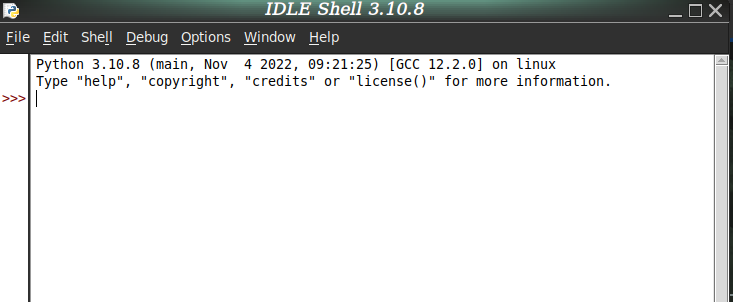
\includegraphics[scale=0.4]{IMG/IDLE-01.png}
\caption{Lancement de l'\textit{IDLE} \texttt{Python}}
\end{center}
\end{figure}
\medskip

A la suite du prompt figuré par les trois chevrons, nous pouvons alors saisir du code \texttt{Python} de façon interactive. L'interface \textit{IDLE} ajoute l'avantage d'afficher les différents éléments syntaxiques dans des couleurs distinctes pour rendre les choses plus lisibles. Une aide contextuelle est aussi fournie.
\medskip

Une autre fonctionnalité intéressante de l'\textit{IDLE} est le rappel des instructions. Les touches \texttt{[Alt] + [p]} (revenir en arrière) et \texttt{[Alt] + [n]} (avancer) permettent de naviguer dans l'historique de saisie des instructions \texttt{Python}.
\medskip

L'\textit{IDLE} \texttt{Python} permet de créer des scripts \texttt{Python} et de travailler directement avec. Pour cela:
\begin{verbatim}
    File  --> New file
\end{verbatim}
\medskip

Une fois votre script enregistré vous pouvez l'exécuter via:
\begin{verbatim}
    Run --> Run Module
\end{verbatim}
\medskip

La sortie apparaît alors dans la fenêtre shell dans l'interpréteur.
\medskip

Pour mieux connaître l'ensemble des fonctionnalités de l'\textit{IDLE} se reporter à la documentation officielle : \url{https://docs.python.org/fr/3/library/idle.html}
\medskip

\subsection*{\texttt{Thonny} un \textit{IDE} pour \texttt{Python}}
\texttt{Thonny} est un \textit{IDE} \texttt{Python} gratuit développé et maintenu par l'Institut d'informatique de l'Université de Tartu, en Estonie. Il s'adresse spécifiquement aux débutants en \texttt{Python}, de sorte que l'interface est simple et épurée et qu'il est facile de la comprendre et de s'y habituer rapidement.
\medskip

Site officiel : \url{https://thonny.org/}
\medskip

\section{Les outils en ligne}
Pour s'exercer à coder depuis n'importe quel ordinateur, où \textit{Python} n'est peut-être pas installé, il est possible de faire appel à des outils en ligne tels que la console interactive du site officiel\footnote{\url{https://www.python.org/shell/}}, \textit{Python Cloud IDE}\footnote{\url{http://pythonfiddle.com/}}, \textit{replit.com}\footnote{\url{www.replit.com}} ou \textit{trinket}\footnote{\url{https://trinket.io/}} qui nous permettent d'écrire du code depuis un navigateur Internet. Si cela peut s'avérer pratique, on ne pourra toutefois pas utiliser des outils avancés.
\medskip

\section{\texttt{Jupyter Notebook}}
\texttt{Jupyter Notebook} est une application \textit{web} qui permet de stocker des lignes de code \texttt{Python}, le résultat de l'exécution du code (notamment des graphiques, tableaux, etc.), ainsi que du texte formaté. Elle offre donc la possibilité d'écrire des petits bouts de code exécutables (insérés dans ce que l'on appelle des \textit{cellules}), de les documenter et d'afficher la résultat de l'exécution. Tout cela est ensuite stocké dans un document partageable. C'est une application fréquemment utilisée par ceux qui travaillent dans l'analyse de données.
\medskip

Installation:
\begin{verbatim}
    # aptitude install jupyter-notebook
\end{verbatim}
\medskip

\texttt{Jupyter Notebook} s'ouvre dans un \textit{navigateur}. Pour créer un \textit{notebook}:
\begin{enumerate}
	\item Cliquer sur \texttt{Nouveau}.
	\item Puis sur \texttt{Python3} (Un nouvel onglet est alors ouvert)
	\item Saisir du code \texttt{Python} dans une \textit{cellule}, puis lancer \texttt{Exécuter}.
\end{enumerate}
\medskip

Il existe quatre types de \textit{cellules}: 
\begin{description}
	\item[\texttt{Code}]: \textit{cellule} qui permet d'insérer du code \texttt{Python}.
	\item[\texttt{Heading}]: type devenu obsolète dans la mesure car avec le type \texttt{markdown} il est beaucoup plus aisé d'insérer des titres.
	\item[\texttt{Text Brut} (pour \texttt{NbConvert}]: permet de contrôler le formatage du document lors d'une conversion du \textit{notebook} en un autre format.
	\item[\texttt{Markdown}]: permet la documentation du \textit{notebook} à l'aide de \textit{balises} \texttt{HTML} ou de la syntaxe \texttt{markdown}\footnote{Pour la syntaxe \texttt{markdown} voir: \url{https://stacklima.com/cellule-markdown-dans-le-bloc-notes- jupyter/}}.
\end{description}
\medskip

%%%%%%%%%%%%%%%%%%%%%%%
%%% Deuxième partie %%%
%%%%%%%%%%%%%%%%%%%%%%%
\part{\textcolor{cyan}{Premiers pas en \textit{Python}: notions de base}}

%%%%%%%%%%%%%%%%%%
%%% Chapitre 1 %%%
%%%%%%%%%%%%%%%%%%
\chapter{Comment cela fonctionne-t-il ?}
\section{Des concepts de base en programmation}
Nous allons progressivement voir et détailler les notions de \textit{variables}, \textit{fonctions}, \textit{boucles}, \textit{conditions} et \textit{algorithmie}. Il s'agit des notions essentielles de base, communes à tous les langages de programmation.
\medskip

Nous pouvons établir une similitude avec la recette de cuisine puisque le développeur, en codant, va finalement écrire une recette. L'ordinateur, à l'instar du cuisinier qui va réaliser la recette de cuisine, sera ensuite à exécuter ce code. Si ce code est bien écrit, alors l'ordinateur va l'exécuter sans difficulté, et le rendu de cette exécution sera celui voulu par le développeur. Au contraire, si le code comporte des erreurs, on dit alors qu'il contient des \textit{bugs} et le rôle du développeur va consister à \textit{déboguer} en analysant le code source, c'est-à-dire à en comprendre les erreurs. Il peut, pour être aidé dans sa tâche, faire appel à un \textit{debugger}, logiciel destiné à investiguer le code en vue de retrouver les erreurs.
\medskip

\section{Les variables}
Une variable est un nom (une étiquette) que l'on associe à une objet. On va alors dire que l'on affecte une valeur à une variable.
\medskip

Exemple:
\begin{verbatim}
    beurre = 50 (Pour des nombres)
    ingredient1 = "lait" (Pour des caractères)
    variable = valeur (syntaxe générale)
\end{verbatim}
\medskip

\section{Les fonctions}
En programmation, une fonction est un bloc de code autonome qui encapsule une tâche spécifique ou un groupe de tâches connexes. Les fonctions vont donc nous permettre de représenter un certain nombre d'actions, et vont aussi nous permettre de mieux structurer et organiser le code.
\medskip

Les fonctions sont capables de retourner (mot clé \texttt{return}) un résultat (une valeur par exemple) que l'on peut ensuite affecter à une variable.
\medskip

\section{Les conditions}
Les conditions, les boucles (cf. infra), mais aussi les fonctions ou les gestions d'erreurs, forment ce que l'on nomme en programmation (notamment utilisées en programmation impérative) les \textit{structures de contrôle}. Les conditions permettent de réaliser des sauts conditionnels en proposant un branchement si une condition est vérifiée. Si la condition n'est pas vérifiée, l'exécution se poursuit séquentiellement. La condition est parfois appelée « condition de rupture » puisqu'elle implique en général une rupture dans le flot d'exécution lorsque la condition est vérifiée. 
\medskip

En \texttt{Python} les conditions fournissent le résultat de l'évaluation d'une expression. Les jeux de \textit{structures de contrôle} que l'on rencontre dans le langage \texttt{Python} sont basés sur des blocs d'instruction balisés par l'indentation, forme syntaxique qui n'utilise pas de mots clés ou de symboles de ponctuation, comme nous pouvons le rencontrer avec d'autres langages de programmation.
\begin{verbatim}
    Si...
        alors...
    Sinon...
\end{verbatim}
\medskip

Exemple avec une recette de cuisine:
\begin{verbatim}
    Si j'ai de la crème
        Alors j'ajoute de la crème
    Sinon
        Je n'ajoute pas de crème
\end{verbatim}
\medskip

Mots clés en programmation pour exprimer les conditions: \texttt{if} (\og \textit{si} \fg{})  et \texttt{else} (\og \textit{sinon} \fg{}).
\medskip

Ainsi, il est possible de réaliser divers tests qui viennent conditionner l'exécution du programme:
\begin{description}
	\item[Le test \og \textit{si} \fg{}]:
	\begin{verbatim}
	    if condition : 
	        instruction
	\end{verbatim}
	\item[Test \og \textit{si sinon} \fg{}]:
	\begin{verbatim}
	    if condition : 
	        instruction 1
	    else:
	        instruction 2
	\end{verbatim}
	\item[Test \og \textit{sinon si} \fg{}]:
	\begin{verbatim}
	    if condition : 
	        instruction 1
	    elif autre condition:
	        instruction 2
	    instruction 3
	 \end{verbatim}
	 \item[Test \og \textit{selon} \fg{}]: en \texttt{Python} cela est possible à partir de la version \texttt{10}, introduit sous le nom \texttt{match case} (cf. le chapitre dédiée aux structures conditionnelles).
\end{description} 

\section{Les boucles}
Une boucle est une structure de contrôle destinée à exécuter une portion de code plusieurs fois de suite.
\begin{verbatim}
    Faire n fois:
        mon action
\end{verbatim}
\medskip

En programmation on rencontre des boucles \texttt{for} et des boucles \texttt{while}.
\bigskip

\section{Algorithmie (ou \og façon de faire \fg{})}
\medskip

\section{Les objets et la programmation orientée objet (\textit{POO)}}
\medskip

%%%%%%%%%%%%%%%%%%
%%% Chapitre 2 %%%
%%%%%%%%%%%%%%%%%%
\chapter{Un premier projet à l'aide d'un \textit{IDE}}
Tout projet \textit{Python} possède la même structure commune de base:
\begin{verbatim}
    - Répertoire (nom du projet)
          |
          |
          ---- Fichier principal (main.py)
\end{verbatim}
\medskip

Plus le projet est important, plus il contiendra de sous répertoires et fichiers (nous verrons cela en temps voulu).
\medskip

\section{Avec \textit{Pycharm}}
Au lancement de \textit{Pycharm} on sélectionne \texttt{New Project}.
\begin{figure}[h]
\begin{center}

\includegraphics[scale=0.3]{IMG/Pycharm-01.png}
\caption{Nouveau projet avec \textit{Pycharm}}
\end{center}
\end{figure}
\medskip

Puis dans la fenêtre qui s'ouvre on va spécifier le répertoire du projet (\texttt{Location}) et l'interpréteur \textit{Python} que l'on va utiliser (\texttt{Base interpreter}). Ensuite, cliquer sur \texttt{Create}. Pour le reste on ne s'en occupe pas pour le moment.
\begin{figure}[h]
\begin{center}
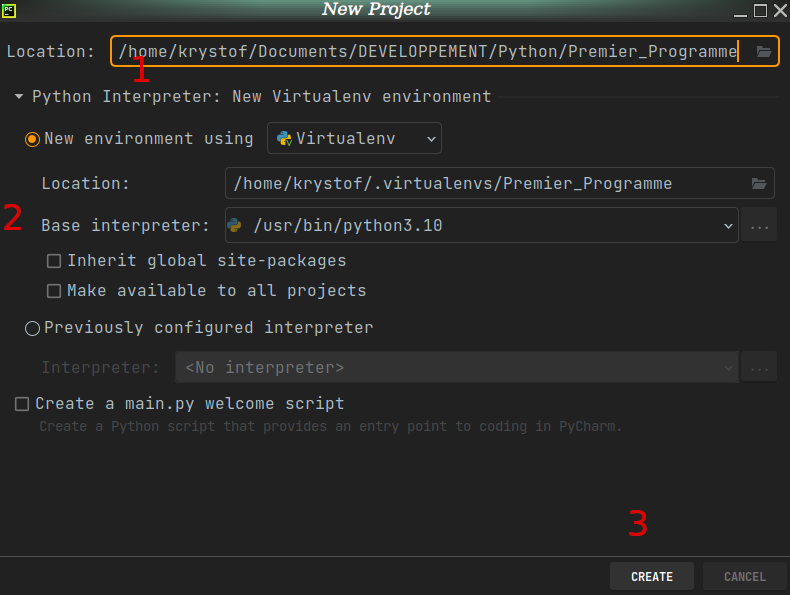
\includegraphics[scale=0.25]{IMG/Pycharm-02.png}
\caption{Création du projet avec \textit{Pycharm}}
\end{center}
\end{figure}
\medskip

Pour créer le premier fichier (notre \texttt{main.py}), faire un clic droit sur le nom du projet qui se situe dans le panneau de gauche (panneau \textit{project}). Sélectionner:
\begin{verbatim}
    New > Python File
\end{verbatim} 
Et nommer ce fichier \texttt{main}.
\begin{figure}[h]
\begin{center}
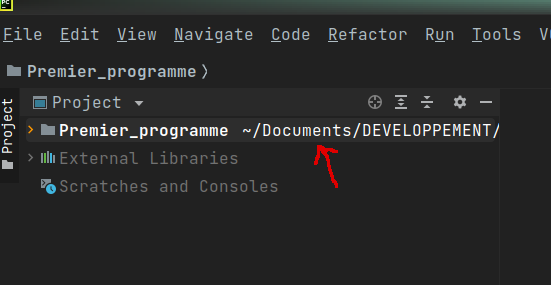
\includegraphics[scale=0.5]{IMG/Pycharm-03.png}
\caption{Premier fichier d'un projet avec \textit{Pycharm}}
\end{center}
\end{figure}
\medskip

Pour illustrer l'exécution du code avec \textit{Pycharm} nous allons tout d'abord insérer la ligne suivante dans le fichier \texttt{main.py}\footnote{\texttt{print()} est une fonction et \texttt{"Bonjour"} son paramètre.}:
\begin{verbatim}
    print("Bonjour")
\end{verbatim}
\medskip

La première fois que l'on lance un programme avec \textit{Pycharm} il faut faire un clic droit sur le panneau de l'éditeur, sélectionner dans le menu déroulant qui s'affiche \texttt{Run "main"}. Cette première fois permet à \textit{Pycharm} de créer une configuration que nous pourrons alors utiliser pour les prochaines exécutions du code, à l'aide du bouton \texttt{Run} en haut à gauche de l'\textit{IDE}.
\begin{figure}[h]
\begin{center}
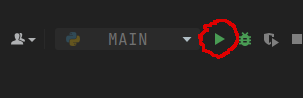
\includegraphics[scale=0.5]{IMG/Pycharm-04.png}
\caption{Lancement du programme avec la touche \texttt{Run}.}
\end{center}
\end{figure}
\medskip

S'ouvre alors le panneau d'exécution du code (panneau \textit{Run}) en bas de l'interface \textit{Pycharm} dans lequel on voit le résultat de notre programme précédé d'une ligne du type:
\begin{verbatim}
    ~/.virtualenvs/Premier_programme/bin/python  ~/Premier_
    programme/main.py
\end{verbatim}
\verb|~/.virtualenvs/Premier_programme/bin/python| représente l'interpréteur auquel nous faisons appel et \verb|~/Premier_programme/main.py| le fichier du code qui sera exécuté.
medskip

\section{Avec \textit{Visual Studio Code}}
Avec \textit{VSC} nous ne sommes pas obligés d'en passer par la création d'un projet. Si le projet ne doit contenir qu'un unique fichier, il peut être en effet plus simple et plus léger d'en passer par cet \textit{IDE}. Pour cela:
\begin{verbatim}
    Fichier > Nouveau fichier > Enregistrer sous
\end{verbatim}
On doit alors choisir le répertoire et donner un nom au fichier qui doit porter l'extension \texttt{.py}.
\medskip

\section{L'exécution du code}
Dans un programme la lecture des lignes de code est séquentielle, un ordre est donc suivi. 
\medskip

Maintenant que nous avons notre premier fichier, nous allons pouvoir entrer dans le coeur du langage \textit{Python} en commençant par aborder les concepts de base.
\medskip

%%%%%%%%%%%%%%%%%%
%%% Chapitre 3 %%%
%%%%%%%%%%%%%%%%%%
\chapter{Les variables}
\section{Une rapide introduction}
\subsection*{Affectation d'une valeur à une variable}
Insérons la ligne suivante dans notre fichier \texttt{main.py}:
\begin{verbatim}
    nom_de_la_personne = "Krystof"
\end{verbatim}
\medskip

A son exécution, rien ne se passe, et pourtant nous venons de créer une nouvelle variable \\(\texttt{nom\_de\_la\_personne}) de type \textit{chaîne de caractères} et qui prend comme valeur la chaîne \texttt{Krystof}. Nous venons donc de stocker la valeur dans la variable. Et dorénavant nous pourrons faire référence à cette variable dès que nous en aurons besoin dans notre code. Une variable doit toujours être définie avant d'être utilisée.
\medskip

Affichons la valeur de notre variable en ajoutant la ligne suivante:
\begin{verbatim}
    print(nom_de_la_personne)
\end{verbatim}
\medskip

Nous pouvons ajouter du texte à cela par une concaténation:
\begin{verbatim}
    print("Bonjour " + nom_de_la_personne)
\end{verbatim}
En \textit{Python}, le symbole \texttt{+} utilisé avec des chaînes de caractères permet donc la concaténation.
\medskip

Il est aussi possible d'afficher de manières successive (avec un espace) les paramètres de la fonction \textit{print()} à l'aide d'une virgule, mais cela n'est pas de la concaténation:
\begin{verbatim}
    print("Bonjour", nom_de_la_personne)
\end{verbatim}
\medskip

Notre code est maintenant composé des deux lignes suivantes:
\begin{lstlisting}
	nom_de_la_personne = "Krystof"
	print("Bonjour " + nom_de_la_personne)
\end{lstlisting}
\medskip

Le résultat une fois ce code exécuté sera:
\begin{verbatim}
    Bonjour Krystof
\end{verbatim}
\medskip

\subsection*{L'évolution d'une variable}
Une variable peut se voir réaffecter une valeur selon le principe suivant:
\begin{description}
	\item[\texttt{n = "Krystof"}]: Création de la variable.
	\item[\texttt{n = "Paul"}]: Réaffectation de la variable. On lui donne simplement une autre valeur.
\end{description}
\medskip

\section{Demander des données à l'utilisateur}
Nous allons réaliser cela à l'aide de la fonction \texttt{input()}. Cette fonction a pour but de retourner une valeur que nous pouvons stocker dans une variable:
\begin{verbatim}
    reponse = input("Quel est votre nom ? ")
\end{verbatim}
\begin{description}
    \item[reponse] = variable
    \item[input()] = fonction
    \item["Quel est votre nom ? "] = paramètre
\end{description}
\medskip

Revenons à notre code qui devient celui-ci:
\begin{lstlisting}
    nom_de_la_personne = input("Quel est votre nom ? ")
    print("Bonjour " + nom_de_la_personne)
\end{lstlisting}
\medskip

A la question posée, on saisit un nom:
\begin{verbatim}
    Quel est votre nom ? Krystof [Entrée]
    Bonjour Krystof
\end{verbatim}
\medskip

\section{Autres types de variables}
\begin{verbatim}
    age = 30
\end{verbatim}
\medskip

Nous venons d'affecter la valeur \texttt{30} à la variable \texttt{age} qui par conséquent devient une variable de type numérique, à la différence de si nous avions codé \verb|age = "30"| où du coup la variable \texttt{age} aurait été de type chaîne de caractères.
\medskip

Il existe une fonction \texttt{type()} qui permet d'indiquer le type d'une variable.
\begin{lstlisting}
    nom = "Krystof"
    age = 30
    print(type(nom))
    print(type(age))
\end{lstlisting}
\medskip

Ce qui donne en sortie:
\begin{verbatim}
    <class 'str'>
    <class 'int'>
\end{verbatim}
\medskip

Nous reviendrons plus tard sur la notions de \textit{classe}. Ce qu'il faut retenir ici c'est que la première variable est identifiée comme \texttt{str} (abréviation de \textit{string} qui veut dire \og chaîne de caractères\fg), et la seconde est identifiée comme \texttt{int} (abréviation de \textit{integer} qui veut dire \og nombre entier\fg).
\medskip

Comme autres valeurs numériques, nous avons les nombres décimaux (de type \texttt{float}), et les booléens dont les valeurs ne peuvent être que \texttt{True} (pour \og vrai \fg, de valeur \texttt{1}) et \texttt{False} (pour \og Faux \fg, de valeur \texttt{0}).
\medskip
  
On ne peut concaténer une chaîne de caractères avec une valeur numérique. Nous aurions alors une erreur de type \texttt{TypeError}. Pour réaliser une telle opération il va nous falloir convertir notre valeur numérique en valeur de type chaîne de caractères. Nous allons utiliser la fonction \texttt{str()}:
\begin{lstlisting}
    age = 30
    print("Notre texte..." + str(age))
\end{lstlisting}
\medskip

La conversion peut aussi se réaliser dans l'autre sens avec la fonction \texttt{int()}.
\begin{lstlisting}[caption=Conversion avec la fonction \texttt{int}]
	age = "30"
	ageX2 = int(age) * 2
	print(ageX2)
\end{lstlisting}
\medskip

Dans le cas présent cela nous affiche \texttt{60}\footnote{Nous n'avons pas encore vu les calculs en \textit{Python}, mais comme vous pouvez le voir sur l'exemple le symbole \texttt{*} correspond au signe de multiplication.}. Par contre si la variable age ne contenait pas une valeur numérique (Si elle avait contenu la valeur \texttt{\og trente \fg} par exemple) nous aurions eu alors une erreur de type \texttt{ValueError}\footnote{Nous reviendrons plus loin sur les erreurs et les types d'erreurs}.
\medskip

En \textit{Python}, les variables peuvent changer de type, ce qui n'est pas possible avec d'autres langages de programmation (Exemple: langage \textit{C}). Mais une telle manipulation est déconseillée. On va alors plutôt faire appel à une autre variable. Il est donc préférable de faire:
\begin{verbatim}
    age_int = int(age)
\end{verbatim}
\medskip

... plutôt que:
\begin{verbatim}
    age = age(int)
\end{verbatim}
\medskip

\subsection*{L'incrémentation d'une variable numérique}
\begin{lstlisting}[caption=Principe de l'incrémentation]
    nbre = 0
    nbre = nbre + 1  # on ajoute 1 à la valeur de la variable
    nbre += 1  # Autre méthode d'incrémentation
\end{lstlisting}
\medskip

\subsection*{La variable de type \texttt{float}}
Il s'agit d'une valeur numérique décimale.
\begin{lstlisting}
  var = 1.75
  print(type(var))
\end{lstlisting}
\medskip

Ce qui donne en sortie:
\begin{verbatim}
    <class 'float'>
\end{verbatim}
\medskip

\section{Les constantes}
En \textit{Python} les variables constantes n'existent pas, mais par convention on va utiliser un nom de variable en lettres majuscules pour indiquer que nous souhaitons utiliser cette variable comme constante, c'est-à-dire que l'on en souhaite pas que sa valeur soit modifiée.
\begin{verbatim}
    MA_CONSTANTE = 100  # Par exemple
\end{verbatim}
\medskip

%%%%%%%%%%%%%%%%%%
%%% Chapitre 4 %%%
%%%%%%%%%%%%%%%%%%
\chapter{Commenter et documenter son code}
\section{L'intérêt de commenter et documenter son code}
Un code est bien plus souvent lu qu'il n'est écrit, et un code bien documenté est un code plus aisément lisible, à la fois pour les autres mais aussi pour soi-même (notamment quand nous devons revenir sur notre code plusieurs semaines après). Daniele \textsc{Procida}\footnote{Directeur de l'ingénierie chez Canonical, responsable de la documentation.} dit : \og \textit{Peu importe la qualité de votre logiciel, car si la documentation n'est pas assez bonne, les gens ne l'utiliseront pas.}\fg{}. Il en est de même pour le code, surtout si nous attendons que d'autres viennent contribuer au projet.
\medskip

Avant d'aller plus avant dans l'apprentissage du langage, apprentissage qui vous permettra de développer des projets de plus en plus fournis en code, nous allons profiter de ce chapitre pour voir comment documenter ce code vous serez amenés à lire et relire, et relire encore. S'il est bien documenter votre relecture en sera souvent bien plus efficace.
\medskip

\section{Le commentaire}
Les commentaires font partie intégrante de tout programme. Il s'agit de lignes de code qui ne seront pas interprétées, et donc ne seront pas exécutées. Ils sont destinés aux développeurs, car ils décrivent des parties du code, lorsque cela s'avère nécessaire, afin d'en faciliter la compréhension des programmeurs, y compris pour vous-même.
\medskip

Exemple d'une ligne de code que l'on ne veut pas interpréter, en mettant le symbole \texttt{\#} devant:
\begin{verbatim}
    # print("Bonjour")
\end{verbatim}
\medskip

On va donc, à l'aide de ce caractère (\texttt{\#}) pouvoir documenter son code, en expliquant en langage commun ce que fait le programme ou telle et telle ligne de code. Il s'agit en fait de notes insérées dans le code. Les commentaires doivent être brefs, ne dépassant pas quelques phrases.
\begin{lstlisting}[caption=Exemple de commentaire]
    # Voici un programme de bienvenue
    # Ici on apprécie les résultats
\end{lstlisting}
\medskip

Les commentaires doivent être courts et précis. Selon la \texttt{PEP 8}\footnote{\url{https://peps.python.org/pep-0008/\#maximum-line-length}}, les commentaires doivent avoir une longueur maximale de 72 caractères. Si la longueur d'un commentaire est supérieure à la limite de caractères, il convient d'utiliser plusieurs lignes pour le commentaire. Deux méthodes sont possibles:
\medskip

1 - L'emploi d'une succession de dièses (\texttt{\#}):
\begin{lstlisting}
def commentaire_multilignes() :
    # Voici un très bon exemple
    # de la façon dont vous pouvez répartir des commentaires
    # sur plusieurs lignes en Python
\end{lstlisting} 
\medskip

2 - L'utilisation des chaînes de caractères avec l'emploi de guillemets triples:
\begin{lstlisting}[caption=Commentaire sur plusieurs lignes]
    """Mon commentaire
    sur plusieurs lignes
    à la fois."""
\end{lstlisting}
\medskip

Bien que cela vous donne la fonctionnalité multi-lignes, ce n'est pas techniquement un commentaire. C'est une chaîne de caractères qui n'est assignée à aucune variable, et qui n'est donc pas appelée ou référencée par votre programme. Cependant, faites attention à l'endroit où vous placez ces \og{} \textit{commentaires}\fg{} multi-lignes. Selon l'endroit où ils se trouvent dans votre programme, ils peuvent se transformer en \textit{docstrings}, qui sont des éléments de documentation associés à une fonction ou à une méthode\footnote{Voir infra, \og \textit{Documenter son code à l'aide des docstrings}\fg{} page \pageref{documenteravecdocstring}}. 
\medskip

\subsection*{Commenter avec un \textit{IDE}}
\subsubsection*{Avec \textit{Pycharm}:}
Sélectionner la partie du code à commenter, puis:
\begin{verbatim}
    Code > Comment with Line Comment
\end{verbatim}
Même opération pour décommenter (ou \texttt{[Ctrl] + [/]} qui est le raccourci clavier).
\medskip

\subsubsection*{Avec \textit{VSC}:}
Une fois la partie de code sélectionnée, pour commenter et décommenter:
\begin{verbatim}
    Edition > Afficher/Masquer le commentaire de ligne
\end{verbatim}
Raccourci clavier: \texttt{[Ctrl] + [Maj] + [:]}
\medskip

Pour commenter/décommenter sur plusieurs lignes (guillemets triples):
\begin{verbatim}
    Edition > Afficher/Masquer le commentaire de bloc
\end{verbatim}
Raccourci clavier: \texttt{[Ctrl] + [Maj] + [A]}
\medskip

\section{Des usages et des règles pour de bons commentaires}
Savoir comment écrire des commentaires en Python peut faciliter la vie de tous les développeurs, y compris la vôtre ! Ils peuvent aider les autres développeurs à comprendre ce que fait votre code, et vous aider à vous familiariser avec votre propre code.
\medskip

Tout d'abord il faut savoir qu'en phase de développement le commentaire permet de rédiger du pseudo-code, comme par exemple décrire une portion de code avant de passer au codage proprement dit de la fonctionnalité ou des instructions que l'on souhaite implémenter.
\medskip

De même, plutôt que d'effacer une portion de code que l'on souhaite modifier, il est possible de la conserver en la commentant. Ainsi si le nouveau code que l'on développe ne fonctionne pas aussi bien que le premier, il sera bien plus facile de réimplémenter celui-ci.
\medskip

\subsection*{Bien commenter}
\begin{itemize}
	\item[-] Avoir des commentaires aussi proches que possible du code décrit;
	\item[-] user d'un formatage simple (éviter les tableaux ou les figures \texttt{ASCII});
	\item[-] ne pas inclure d'informations redondantes;
	\item[-] concevoir un code qui se commente lui-même\footnote{Voir à ce sujet les annotations de type page \pageref{annotation_types}.}.
\end{itemize}
\medskip

\subsection*{Des commentaires inutiles}
\begin{itemize}
	\item[-] Eviter les redondances du type:
	\begin{lstlisting}
	return a  # Retourne a
	\end{lstlisting}
	\item[-] Des commentaires qui peuvent s'éviter si le noms donnés aux variables sont suffisamment explicites
	\begin{lstlisting}
	v = 4  # Nombre de vies
	# Vaut mieux coder:
	nbre_de_vies = 4
	\end{lstlisting}
	\item[-] Les commentaires doivent rarement être plus longs que le code qu'ils soutiennent.
\end{itemize}
\medskip

\section{Commenter \textit{vs} documenter}
En général, commenter consiste à décrire votre code, afin d'aider le travail des mainteneurs et des développeurs du code. Associés à un code bien écrit, les commentaires aident le lecteur à mieux comprendre votre code, son objectif et sa conception. Le code vous décrit la façon, les commentaires vos indiquent le but poursuivi.
\medskip

Documenter le code, c'est décrire son utilisation et ses fonctionnalités à vos utilisateurs. Bien que cela puisse être utile dans le processus de développement, le principal public visé est constitué par les utilisateurs.
\medskip

\section{Documenter son code à l'aide des \textit{docstrings}}\label{documenteravecdocstring}
Outre les commentaires il est possible de documenter son code à l'aide de \textit{docstrings}. Cette documentation sera abordée tout au long du chapitre \textit{Documenter son code et son projet} page \pageref{documentercodeprojet}, mais avant cela nous devrons d'abord aborder diverses notions essentielles de programmation en \texttt{Python}.
\medskip
 
 \section*{Sources pour la rédaction de ce chapitre}
\begin{description}
	\item[Writing Comments in Python (Guide)] - trad: \og \textit{Écrire des commentaires en Python (Guide)} \fg{} - Par Jaya \textsc{Zhané} - 5 novembre 2018 - \url{https://realpython.com/python-comments-guide/}
\end{description}
\medskip

%%%%%%%%%%%%%%%%%%
%%% Chapitre 5 %%%
%%%%%%%%%%%%%%%%%%
\chapter{Erreurs et gestion des exceptions}
\section{Les exceptions: tester son code}
Dans cette partie on va utiliser des blocs de codes. En langage \textit{Python} un bloc de codes s'initie par le double points (\texttt{:}). Puis concernant les lignes de code qui font partie de ce bloc on les insère après une tabulation. En \textit{Python} la tabulation fait partie de la syntaxe du langage. Dans d'autres langages comme le \textit{C} ce sont les accolades qui délimitent les blocs de codes.
\medskip

\begin{lstlisting}
try:  # Indique de tester le code qui suit
    age = int(age)
except:  # Si ça ne fonctionne pas...
    print("ERREUR: vous devez saisir un nombre")
else:  # Si la ligne sous le try fonctionne...
    print("Vous avez " + age + " ans.")
\end{lstlisting}
\medskip

A partir de la ligne avec \texttt{except} nous introduisons une condition à notre code.
\medskip

Syntaxe de \texttt{try}...\texttt{except}...\texttt{else}:
\begin{lstlisting}
try:
    ...code testé...
except:
    ...code exécuté si le test échoue...
else:
    ...code exécuté si le test est réussi...
\end{lstlisting}
\medskip

\texttt{except} seul ne va lever une exception que de façon générique. L'exception peut être levée en raison d'une erreur de syntaxe alors que nous avons prévu notre exception pour lever une erreur de type. Il est cependant possible de spécifier le type d'erreur et d'indiquer dans le bloc de codes de gestion d'exception, et même d'y lever plusieurs exceptions en fonction du type d'erreur. Toutefois, il est déconseillé de mettre toutes les lignes de codes dans un même bloc \texttt{try}, mais plusieurs blocs de \texttt{try} successifs sont envisageables.
\medskip

Ainsi pour lever une exception d'erreur de type, notre \texttt{except} peut s'écrire de la façon suivante:
\begin{verbatim}
    except ValueError:
\end{verbatim}
\medskip

A noter qu'un \texttt{except} seul est surligné dans \textit{Pycharm}.
\medskip

\section{Afficher le message d'erreur}
Il est possible de capturer l'exception et d'afficher le message d'erreur idoine à l'aide du mot clé \texttt{as}
\begin{lstlisting}
try:
    # Bloc de code à tester
except TypeException as msg_exception:
    print(f"Voici l'erreur {msg_exception}")
\end{lstlisting}
\medskip

\section{Lever soi-même des exceptions}
Par exemple, cela peut nous servir à invalider des saisies utilisateurs, alors que cette saisie peut être considérée comme correcte vis-à-vis du code. On utlise pour cela le mot clé \texttt{raise}.
\medskip

\chapter{La boucle \texttt{while}}
Cette boucle veut dire \textit{tant que...}. C'est est une structure de contrôle permettant d'exécuter un ensemble d'instructions de façon répétée sur la base d'une condition booléenne. Exemple simple d'introduction à la logique des boucles \texttt{while}:
\begin{lstlisting}[caption=Premier exemple avec la boucle \textit{while}]
    n = 0  # 0 = valeur d'initialisation souvent prévue par défaut
    while n < 10:  # On peut utiliser les signes: > < >= <= ==
        print("n = " + str(n))
        n = n + 1  # Incrémentation. Sortie de boucle quand n = 10
\end{lstlisting}
\medskip

Avec la boucle \texttt{while} on introduit une condition qui nous permet de faire évoluer des variables. Une boucle \texttt{while} est constituée d’un bloc de code source et d’une condition. À l’exécution, la condition est d’abord évaluée, et si elle est vraie, le bloc de code source est évalué. L'exécution du code est ensuite répétée jusqu’à ce que la condition soit fausse. 
\medskip

Autre exemple avec une condition du type \textit{Tant que n'est pas égal à...}:
\begin{lstlisting}[caption=Deuxième exemple avec la boucle \textit{while}]
    mdp = ""  # Initialisation de la variable pour tester une
              # première fois la boucle while
    while not mdp == "123":
        mdp = input("Quel est le mode passe ? ")
    print("Mot de passe correct !")
\end{lstlisting}
\medskip

Autre exemple:
\begin{lstlisting}[caption=Troisième exemple avec la boucle \textit{while}]
    age = 0  # Valeur d'initialisation de la variable que nous allons  
             # utiliser pour 'boucler'
    while age == 0:
        age_str = input ("Quel age avez-vous ? ")
        try: 
            age = int(age_str)  # Si cela ne fonctionne pas, la  
                                # valeur de la variable 'age' reste  
                                # à 0, et donc on demeure dans la
                                # boucle
        except ValueError:
            print("ERREUR: saisir un nombre.")
    # Une fois sorti de la boucle:
    print("Vous avez " + str(age) + " ans.")  
\end{lstlisting}
\medskip

%%%%%%%%%%%%%%%%%%
%%% Chapitre 7 %%%
%%%%%%%%%%%%%%%%%%
\chapter{Le debogage}
Une des activités centrales d'un développeur est le \textit{débogage} qui va consister à tester et rechercher les erreurs dans son code. Les \textit{IDE} \texttt{Pycharm} et \texttt{Visual Studio Code}, dotés d'un débogueur, vont nous permettre d'investiguer les erreurs dans notre code. L'intérêt du \textit{débogage} est aussi de pouvoir consulter l'état de nos \textit{variables} tout en observant comment le code est exécuté. Apprendre le débogage dès le début de son apprentissage du langage \texttt{Python} offre ainsi des avantages, notamment dans le suivi pas à pas de l’exécution de notre code. Le débutant, pour visualiser le contenu de ses objets mutables (\textit{variables}, \textit{listes}, etc.) sera tenté de parsemer son code de diverses \textit{fonctions} d'affichages (les fameux \texttt{print()}). Utiliser le \textit{débogage} fait donc parti des bonnes habitudes à acquérir rapidement. C'est pourquoi il est ici proposé avant d'aller plus en avant dans l'apprentissage du code. 
\medskip

\section{\textit{Pycharm}}
\subsection*{Activer le mode débogage}
Entre le numéro de ligne de code et la ligne de code il y a une colonne. Cliquer au niveau d'une ligne de code: un point rouge apparaît. Il s'agit d'un point d'arrêt (\textit{break point}).
\begin{figure}[h]
\begin{center}
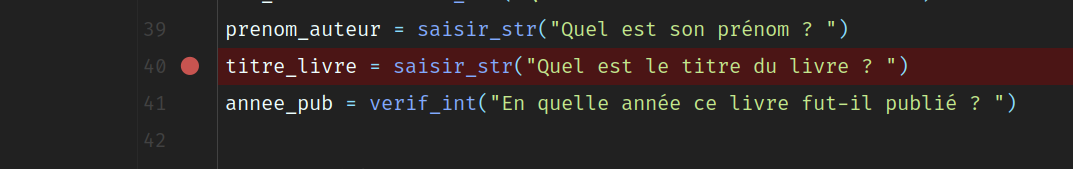
\includegraphics[scale=0.3]{IMG/Pycharm-05.png}
\caption{\textit{Pycharm} - Activer le débogage}
\end{center}
\end{figure}
\medskip

Lancer ensuite le mode débogage en cliquant sur l'icône en forme d'insecte en haut à droite.
\begin{figure}[h]
\begin{center}

\includegraphics[scale=0.6]{IMG/Pycharm-06.png}
\caption{\textit{Pycharm} - Lancer le débogage}
\end{center}
\end{figure}
\medskip

Quand le programme atteint le point d'arrêt, son exécution s'arrête, et nous pouvons alors observer ce qu'il s'est passé.
\begin{figure}[h]
\begin{center}
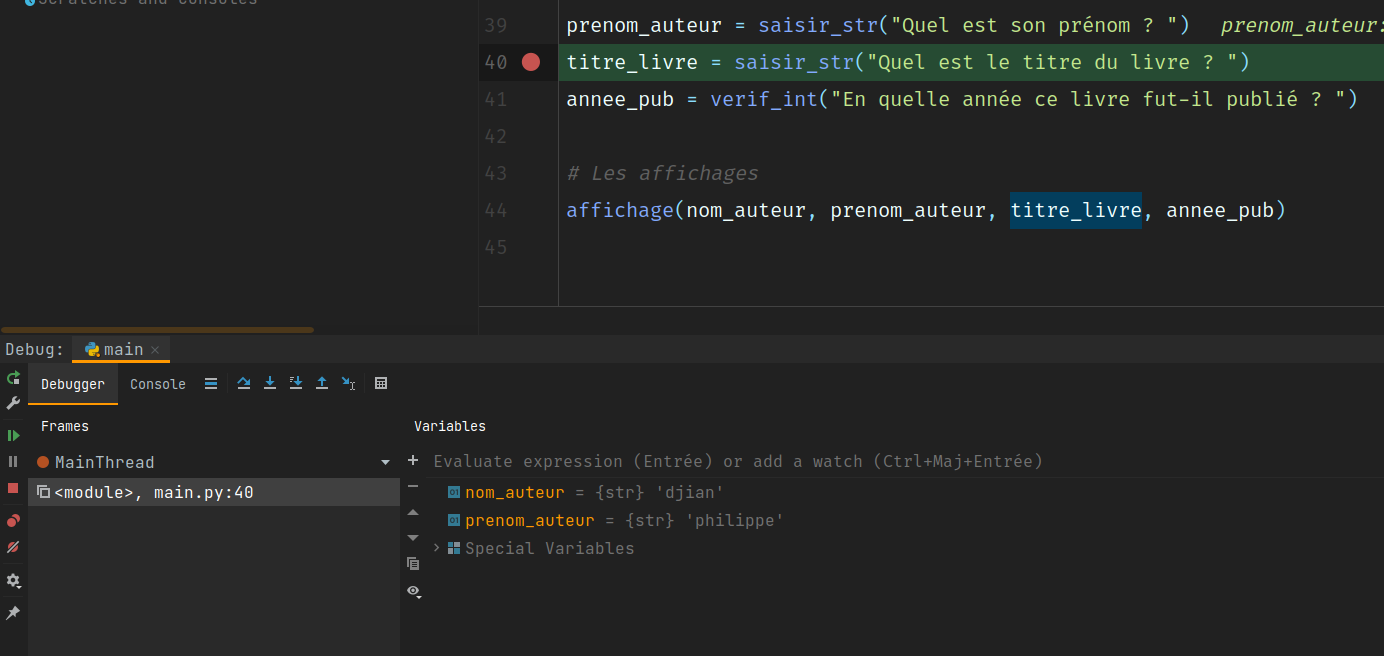
\includegraphics[scale=0.3]{IMG/Pycharm-07.png}
\caption{\textit{Pycharm} - Arrivée au point d'arrêt}
\end{center}
\end{figure}
\medskip

\subsection*{Poursuivre l'exécution du code en mode débogage}
Dans le panneau \textit{debug}, cliquer sur le panneau \textit{Step Over} (ce qui veut dire \textit{Étape suivante}.
\begin{figure}[h]
\begin{center}
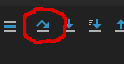
\includegraphics[scale=0.6]{IMG/Pycharm-08.png}
\caption{\textit{Pycharm} - Le bouton \textit{Step Over}}
\end{center}
\end{figure}
\medskip

En avançant ainsi dans le code, il est possible que nous soyons bloqué face à une instruction de type \texttt{input()}. Il faut alors revenir sur le panneau \textit{Console} et saisir ce qui nous est demandé par le code.
\medskip

\section{\textit{Visual Studio Code}}
\subsection*{Activer le mode débogage}
Le point d'arrêt se fixe par simple clic juste à gauche du numéro de ligne choisi.
\begin{figure}[h]
\begin{center}
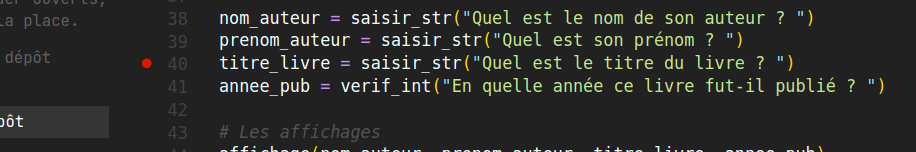
\includegraphics[scale=0.3]{IMG/VSC-01.png}
\caption{\textit{VSC} - Activer le débogage}
\end{center}
\end{figure}
\medskip

Lancer le débogage:
\begin{verbatim}
    Exécuter > Démarrer le débogage
\end{verbatim}
\medskip

Lors du premier lancement s'ouvre une fenêtre (\textit{Select a debug configuration}): sélectionner \textit{Python File}. Puis l'exécution du programme stoppe au niveau du point d'arrêt.
\begin{figure}[h]
\begin{center}
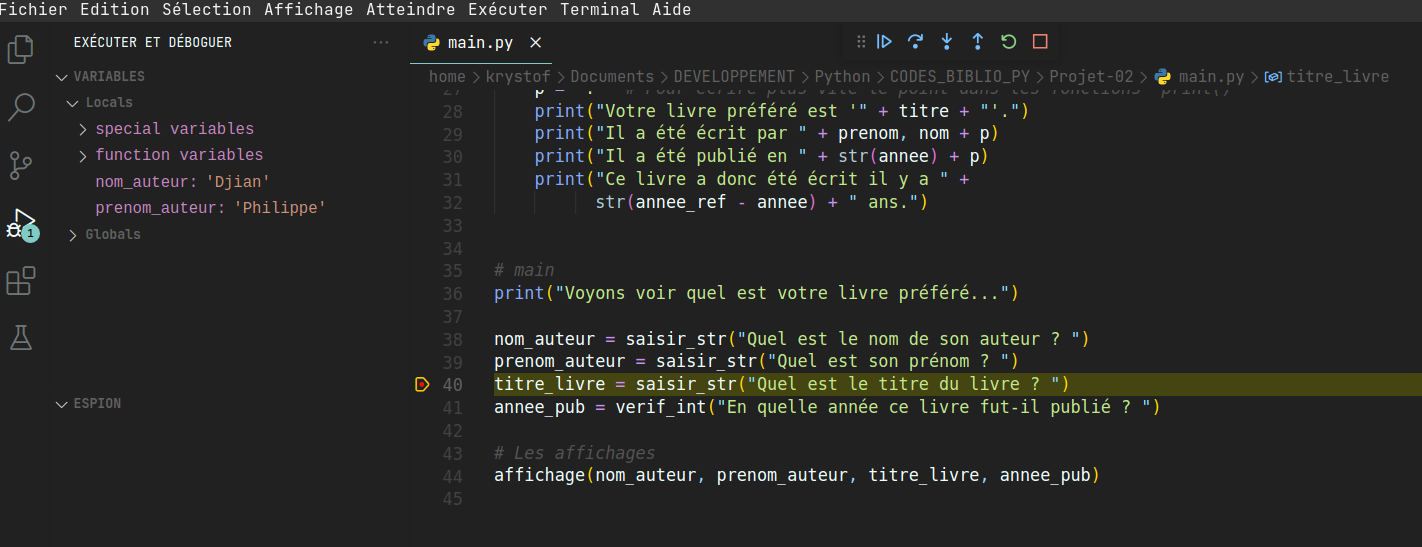
\includegraphics[scale=0.3]{IMG/VSC-02.png}
\caption{\textit{VSC} - Arrivée au point d'arrêt}
\end{center}
\end{figure}
\medskip

\subsection*{Poursuivre l'exécution du code en mode débogage}
Grâce au bouton \textit{Pas à pas principal}.
\begin{figure}[h]
\begin{center}
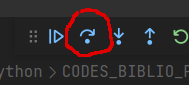
\includegraphics[scale=0.6]{IMG/VSC-03.png}
\caption{\textit{VSC} - Le bouton \textit{Pas à pas principal}}
\end{center}
\end{figure}
\medskip

\chapter{Les fonctions}
\section{Quel est l'intérêt des fonctions ?}
Les \textit{fonctions} sont fondamentales en programmation. Elles sont des éléments clés qui vont nous permettre de structurer notre code et d'en améliorer la qualité, en évitant d'avoir recourt à des répétitions de code\footnote{En pratique un projet (ou programme) va contenir une fonction principale (\texttt{def main()}) qui va, comme son nom l'indique contenir le code principal, et c'est à partir de cette fonction principale que seront appelées la plupart des autres fonctions.}. Ce sont des objets dits \textit{callables} (\og \textit{appelables}\fg{} pourrait-on traduire) qui sont associés à des actions. Pratiquement tous les langages de programmation utilisés aujourd'hui prennent en charge des fonctions définies par l'utilisateur, même si elles ne sont pas toujours appelées fonctions. Dans d'autres langages, elles peuvent être désignées par l'un des termes suivants : \textit{sous-routines} (\textit{subroutines}), \textit{procédures} (\textit{procedures}), \textit{méthodes} (\textit{methods}), \textit{sous-programmes} (\textit{subprograms}).
\medskip

A l'aide des fonctions, notamment dans le développement de projets conséquents, nous saurons proposer un code aisément maintenable\footnote{A noter que si l'on sur-structure un code avec des fonctions qui n'ont pas lieu d'être, il est très aisé de le destructurer.}. Les fonctions vont donc nous offrir la possibilité d'avoir:
\begin{description}
	\item[Un code réutilisable]: vous disposez d'une portion de code que vous avez besoin de reproduire à divers endroits de votre projet, et bien plutôt que de venir \textit{copier-coller} ce code à tous ces endroits, vous pouvez simplement \textit{encapsuler} ce code dans une fonction, et uniquement depuis les endroits où vous en avez besoin vous pouvez alors faire appel à ce morceau de code. Ce qui le rend d'ailleurs plus maintenable car si vous souhaitez le modifier il n'y a plus que le code de la fonction à modifier, et ce une seule fois au lieu de toutes les portions que vous auriez pu \textit{copier-coller} par-ci par-là dans le code du projet\footnote{\og \textit{Don't repeat yourself}\fg{} (aussi désigné par l’acronyme \textit{DRY} - trad. \og \textit{Ne vous répétez pas}\fg{}) est une philosophie en programmation informatique consistant à éviter la redondance de code au sein d’une application afin d'en faciliter sa maintenance, les tests, le débogage et les évolutions de cette dernière.}.
	\item[Un code modulaire]: les fonctions permettent de décomposer des processus complexes en étapes plus petites. Au lieu de regrouper tout le code de façon linéaire et continue, nous pouvons le diviser en fonctions distinctes, chacune d'entre elles se concentrant sur une tâche spécifique. Le fait de diviser une tâche importante en petites sous-tâches permet de la gérer plus facilement. Au fur et à mesure que les programmes se compliquent, il devient de plus en plus avantageux de  modulariser les tâches plus ou moins complexes qu'il est censé accomplir.
	\item[Un code avec des \textit{espaces de noms} bien distincts]: un espace de noms est une région d'un programme dans laquelle les identifiants ont une signification. Lorsqu'une fonction \texttt{Python} est définie, un nouvel espace de noms est créé pour cette fonction, un espace distinct de tous les autres espaces de noms existants. Le résultat pratique est que des variables peuvent être définies et utilisées dans une fonction même si elles portent le même nom que des variables définies dans d'autres fonctions ou dans le programme principal. Dans ces cas, il n'y aura pas de confusion ou d'interférence car elles sont conservées dans des espaces de noms distincts. Cela signifie que lorsque vous écrivez du code à l'intérieur d'une fonction, vous pouvez utiliser des noms de variables et des identificateurs sans vous soucier de savoir s'ils sont déjà utilisés ailleurs en dehors de la fonction. Cela permet de minimiser considérablement les erreurs dans le code.
\end{description}
\medskip

\section{Comment ça fonctionne ?}
\subsection*{Première étape : la définition (ou implémentation) d'une fonction}
A l'instar des variables, définir une fonction c'est lui donner un nom (une étiquette). Sa définition est finalement une affectation cachée. Une fonction est une boîte de codes (on parle d'\textit{encapsulation} du code) à laquelle nous passons des \textit{paramètres} lors de son \textit{appel}.
\begin{verbatim}
    def nom_fonction(paramètres):
        ...code de la fonction...
        ...ou bloc d'instructions...
\end{verbatim}
\medskip

Une fonction ne se définit qu'une seule fois, mais nous pouvons l'appeler (cf. infra \textit{L'appel de fonction}) autant de fois que nous le souhaitons. Généralement on place les définitions de fonctions en début de code\footnote{Deux fonctions sont séparées par deux lignes vides}. Au lancement du programme, elle ne sera pas exécutée. Seuls les noms des fonctions seront lus. Il faut la considérer comme du code séparé. Une fonction n'est exécutée que lors de son appel.

\subsection*{Seconde étape : l'appel de fonction}
On appelle une fonction (cet appel implique que la fonction existe déjà) en fournissant son nom suivi de parenthèses. L'appel sans les parenthèses ne fera que l'afficher, au même titre que n'importe quel objet.
\medskip

\begin{lstlisting}[caption=Utiliser une fonction]
def afficher():
    print("Mon texte affiché")


afficher()  # Appel
print(afficher)  # Affichage
\end{lstlisting}
\medskip

Ce petit bout de code produira en sortie:
\begin{verbatim}
    Mon texte affiché
    <function afficher at 0x7f820b269d80>
\end{verbatim}
\medskip

Une variable se définit dans un contexte. Une variable définit dans le contexte d'une fonction ne sera pas accessible en dehors de la fonction, car elle n'existe que pour la fonction et non pour le programme principal. Pour permettre à une variable d'exister en dehors de la fonction, et d'être utilisée par le programme principal, on va retourner cette variable à l'aide du mot-clé \texttt{return}\footnote{Mot-clé qui ne s'utilise qu'à l'intérieur d'une fonction}. Du contenu de la fonction, le programme principal n'y a pas accès, il n'aura accès qu'à ce qui est retourné. Mais il faut savoir qu'une fonction ne retourne pas nécessairement quelque chose de façon explicite (par défaut la valeur de retour est \texttt{None}).
\medskip

\begin{lstlisting}[caption=Un premier exemple de fonction]
def dder_age():  # Notre fonction
    age_int = 0
    while age_int == 0:
        try:
            age_int = int(input("Quel âge avez-vous ? "))
        except ValueError:
            print("Erreur: veuillez saisir un nombre.")
    return age_int

# Code principal
print("Bonjour")
age = dder_age()
print(f"Vous avez {age} ans.")
\end{lstlisting}
\medskip

\subsection*{Les fonctions intégrées à \textit{Python} grâce à la bibliothèque standard}
Il existe, à l'instar de la fonction \texttt{print()}, un certain nombre de fonctions contenues dans la bibliothèque standard de \texttt{Python}. On parle alors de \textit{fonctions natives}. Il y a des fonctions qui exécutent du code (Exemple de la fonction \texttt{print()}), et des fonctions qui retournent des valeurs (Exemple de la fonction \texttt{input()}\footnote{La fonction \texttt{input()} a en plus la caractéristique d'être bloquante, et seul le fait de presser la touche \texttt{[Entrée]} nous fait sortir de la fonction et permet l'exécution de la suite du code.}), valeur que l'on récupère dans une variable.
\medskip

Voyons deux exemples de fonctions natives : \texttt{len()} et \texttt{type()}.\texttt{len()} est une fonction qui nous permet d'obtenir la longueur d'une chaîne de caractères. On lui passe une chaîne de caractères en paramètre et elle retourne un objet de type \texttt{int}. \texttt{type()} est aussi une fonction intégrée issue de la bibliothèque standard.
\begin{lstlisting}[caption=Les fonctions \texttt{len()} et \texttt{type()}]
a = "Python"
b = len(a)
print(b)
print(type(a))
print(type(b))
\end{lstlisting}
\medskip

Sortie dans la console: 
\begin{verbatim}
    6
    <class 'str'>
    <class 'int'>
\end{verbatim}
\medskip

Il en existe encore plein d'autres fonctions issues de la bibliothèque standard avec chacune leurs spécificités, que ce soit au niveau des entrées et des sorties.
\medskip

\section{La définition d'une fonction}
Créer une fonction signifie que l'on \og définit\fg{} une fonction, ou qu'on l'\og{}implémente\fg{}. La syntaxe habituelle pour définir une \textit{fonction} \texttt{Python} est la suivante:
\begin{verbatim}
    def nom_fonction(arguments):
        ...bloc d'instructions...
\end{verbatim}
\medskip

Décortiquons cela:
\begin{description}
	\item[\texttt{def}]: mot-clé pour définir une fonction.
	\item[\texttt{nom\_fonction}]: identificateur de la fonction. Les conditions de nommage d'une fonction (de l'identificateur) sont les mêmes que pour les variables.
	\item[(arguments)]: ils sont optionnels, et séparés par des virgules quand il y en a plusieurs. Ils correspondent aux paramètres qui sont passés à la fonction. Vous pouvez définir une fonction qui ne prend aucun \textit{argument}, mais les parenthèses sont toujours nécessaires.
	\item[Les deux points (\texttt{:})]: ponctuation qui indique la fin de l'\textit{en-tête} (nom et arguments) de la fonction, et que nous allons débuter un \textit{bloc d'instructions} (de code).
	\item[L'\textit{indentation}]: tout bloc d'instructions respecte, en \texttt{Python}, les règles de l'indentation. Ce bloc d'instructions correspond au \textit{corps de la fonction} qui sera exécuté à chaque appel de la fonction.
\end{description}
\medskip

Une fonction doit être définie avant son appel, sur le même principe que pour les variables. Dans un codage \og propre\fg{} on les retrouve au début du code, avant le lancement de la première ligne d'instructions.
\medskip

Dans l'idéal, une fonction doit avoir une limite se situant autour d'une vingtaine de lignes de code. Au-delà, elle risque d'être longue et certainement mériterait-elle un découpage faisant appel à d'autres fonctions. Une fonction doit, en pratique, ne faire qu'une seule et unique action, mais la faire proprement et de façon à être aisément réutilisable.
\medskip

\section{L'appel de la \textit{fonction}}
La syntaxe pour appeler une \textit{fonction} est la suivante:
\begin{verbatim}
    nom_fonction(paramètres)
\end{verbatim}
\medskip

L'appel de la fonction permet l'exécution de la fonction, c'est-à-dire l'exécution du bloc d'instructions qu'elle contient. Ce n'est qu'à la suite de son appel qu'une fonction sera exécutée, sinon elle demeure ignorée. Sa définition permet au programme qu'elle soit connue et identifiée, mais son contenu demeure opaque tant qu'elle n'est pas appelée.
\medskip

S'il n'y a aucun paramètre passé à la fonction son appel doit tout de même comporter des parenthèses (à l'instar de sa définition).
\medskip

Quand il n'y a plus d'instructions à exécuter au sein de la fonction, elle retourne ce qui est explicitement attendu (une valeur que l'on va affecter à une variable, par exemple) par le mot-clé \texttt{return}, ou bien elle retourne un objet implicite (pas besoin du mot-clé \texttt{return}) qui est de type \texttt{None}.
\begin{lstlisting}[caption=Exemple du fonctionnement d'une fonction]
def nom_poete():
    return "Charles BAUDELAIRE"


print("Qui a écrit 'Les Fleurs du Mal' ?")
nom = nom_poete()  # Appel de la fonction et valeur de retour
                   # de la fonction affectée à une variable.
print(f"C'est {nom}")  # Ligne exécutée après l'exécution de  
                       # la fonction.
\end{lstlisting}
\medskip

La sortie en console sera alors:
\begin{verbatim}
    Qui a écrit 'Les Fleurs du Mal' ?
    C'est Charles BAUDELAIRE
\end{verbatim}
\medskip

\section{Variable globale et paramètres}
L'intérêt des fonctions résident aussi dans la passage de paramètres (de données) qui vont interagir sur le comportement de la fonction. Ces paramètres vont s'utiliser tels des variables nécessaires à l'exécution du bloc d'instructions.
\medskip

\subsection*{Variable locale \textit{vs} variable globale}
Une variable à l'intérieur d'une fonction est une \textit{variable locale}, locale à la fonction.
\medskip

Avant la définition d'une fonction il est possible de définir une variable au sein du programme principal. Il s'agit alors d'une \textit{variable globale}. Pour que la fonction prenne en considération une telle variable, on va alors au sein de la fonction utiliser l'instruction \texttt{global nom\_variable}. Le code de la fonction peut être, par exemple, une simple incrémentation de la valeur de cette variable. Alors un simple appel de la fonction viendra incrémenter la valeur de la variable, et il n'y aura pas nécessité de recourir à l'instruction \texttt{return nom\_variable} puisque étant globale elle sera directement modifiée au sein du programme principal. Mais une telle manipulation est à éviter car la fonction est alors dépendante des variables définies à l'extérieur de la fonction. Et justement, l'intérêt d'une fonction réside dans son indépendance et sa modularité. Elle doit pouvoir s'utiliser par ailleurs.
\medskip

\begin{lstlisting}[caption=Fonction et variable globale]
variable = 0


def fction():
    global variable
    variable += 10


print(variable)  # Avant le premier appel de fonction
fction()  # Premier appel de fonction
print(variable)
fction()  # Second appel de fonction
print(variable)
\end{lstlisting}
\medskip

Sortie en console:
\begin{verbatim}
    0
    10
    20
\end{verbatim}
\medskip

A noter qu'il est possible pour une fonction d'utiliser une variable définie globalement, et sans avoir à recourir au mot-clé \texttt{global}, mais sachez que cette variable ne sera accessible qu'en lecture, et non en écriture, donc non modifiable au niveau global comme nous l'avons vu précédemment.
\medskip

\subsection*{Les paramètres de fonctions - Les variables locales}
Pour permettre à une fonction d'utiliser une variable définie ailleurs (à l'extérieur de la fonction), on va lui donner cette variable sous la forme d'un argument que l'on va passer en paramètre lors de l'appel. Ce paramètre est la valeur ou la variable que l'on souhaite passer à notre fonction. Dans certains textes consacrés à la programmation, les arguments donnés dans la définition de la fonction sont appelés \textit{paramètres formels}, et les paramètres passés dans l'appel de la fonction sont appelés \textit{paramètres réels} :
\begin{lstlisting}[caption=Exemple de fonction avec paramètre]
def double(a):
  return a * 2
	
print(double(7))
\end{lstlisting}
\medskip

Cela nous affichera la valeur \texttt{14} qui est retournée par notre fonction \texttt{double()}. A noter qu'ici la fonction \texttt{print()} a pour paramètre l'appel de la fonction \texttt{double()}. Nous venons de voir la façon la plus simple de transmettre des arguments à une fonction \texttt{Python} par l'utilisation d'un \textit{argument positionnel} (également appelé \textit{argument requis}, \og \textit{required argument}\fg{} en anglais). Dans la définition de la fonction, il est possible de spécifier une liste de paramètres que l'on sépare alors par des virgules :
\medskip
\begin{lstlisting}[caption=Fonction avec plusieurs arguments positionnels]
def affiche_texte(nom, prenom, titre):
    return f"{prenom.capitalize()} {nom.upper()} a écrit " \
           f"'{titre.title()}'"


auteur_nom = "hemingway"
auteur_prenom = "ernest"
titre_livre = "pour qui sonne le glas"
print(affiche_texte(auteur_nom, auteur_prenom, 
                    titre_livre))
\end{lstlisting}
\medskip

La sortie du code sera la suivante:
\begin{verbatim}
    Ernest HEMINGWAY a écrit 'Pour Qui Sonne Le Glas'
\end{verbatim}
\medskip

Lorsque la fonction est appelée, la liste d'arguments spécifiée doit correspondre aux paramètres précisés lors de la définition de la fonction. Bien que les arguments positionnels constituent le moyen le plus simple de transmettre des données à une fonction, ils offrent également le moins de flexibilité. En effet, l'ordre des arguments dans l'appel doit correspondre à l'ordre des paramètres dans la définition. Avec les arguments positionnels, les arguments de l'appel et les paramètres de la définition doivent concorder non seulement dans l'ordre mais aussi en nombre. C'est également la raison pour laquelle les arguments positionnels sont également appelés arguments requis. Vous ne pouvez en omettre aucun lors de l'appel de la fonction.
\medskip

L'utilisation des paramètres va finalement rendre nos fonctions beaucoup plus modulaires. L'intérêt d'une fonction réside justement dans son aspect générique, nous offrant alors la possibilité de faire appel selon divers cas de figure. Et il faut bien garder à l'esprit que les paramètres se comportent comme des variables définies localement (uniquement accessibles dans le corps de la fonction).
\medskip

Les noms données aux paramètres et aux arguments sont différents, mais rien ne vous empêche d'utiliser les mêmes, car les valeurs associées seront exploités uniquement par la fonction, le programme principal n'y ayant pas accès. Cela n'a donc aucune importance.
\medskip

Cependant l'ordre des paramètres et arguments a son importance, car sinon la fonction ne recevrait pas les bons arguments. De même pour le nombre: une fonction devant recevoir deux arguments ne peut en recevoir trois. Si tel était le cas, l'exécution du programme stopperait et une exception de type \texttt{TypeError} serait levée. 
\medskip

\subsection*{Paramètre optionnel}
Un paramètre peut être rendu optionnel en lui donnant une valeur par défaut. Et il permet d'éviter de \textit{lever une exception} si l'argument n'est pas passé à la fonction. Il est toujours placé après les paramètres qui ne sont pas optionnels.
\medskip

\begin{verbatim}
    def ma_fonction(var1, var2, var3=0):  # var3 = paramètre otpionnel
\end{verbatim}
\medskip

Et pour appeler la fonction:
\begin{verbatim}
    ma_fonction(var1, var2)
\end{verbatim}
\medskip

En donnant une valeur par défaut au paramètre \texttt{var3}, on rend l'argument optionnel pour l'appel de la fonction.
\medskip

\subsection*{Argument et paramètre par \textit{mot-clé}}
Il est aussi possible, lors de l'appel de fonction de donner le nom du paramètre auquel on affecte une valeur:
\begin{verbatim}
    ma_fonction(var1, var2=4)
\end{verbatim}
\medskip

Une affectation explicite (par mot-clé) est plus intuitive qu'une affectation positionnelle\footnote{Dans \textit{The Zen of Python} il est d'ailleurs dit: \og \textit{Explicit is better than implicit}\fg{}.}. L'utilisation d'arguments de type mot-clé lève la restriction sur l'ordre des arguments. Chaque argument mot-clé désigne explicitement un paramètre spécifique par son nom. Vous pouvez donc les spécifier dans n'importe quel ordre et \texttt{Python} saura toujours quel argument va avec quel paramètre. Ainsi, les arguments de type mot-clé permettent une certaine flexibilité dans l'ordre dans lequel les arguments de la fonction sont spécifiés, mais le nombre d'arguments reste rigide, car comme pour les arguments positionnels, le nombre d'arguments et de paramètres doit toujours correspondre. Par ailleurs, la référence à un mot-clé qui ne correspond à aucun des paramètres déclarés lève une exception de type \texttt{TypeError}.
\medskip

Il est à noter que vous pouvez appeler une fonction en utilisant à la fois des arguments positionnels et des mots-clés. Une fois que vous avez spécifié un argument de type mot-clé, il ne peut y avoir aucun argument positionnel à sa droite.
\medskip

\section{Les retours de fonction}
Le mot-clé \texttt{return} sert à deux choses:
\begin{enumerate}
	\item Sortir de la fonction. Avec des structures conditionnelles cela peut avoir son utilité.
	\item Potentiellement à renvoyer une valeur (non obligatoire), c'est-à-dire l'objet fabriqué dans la fonction.
\end{enumerate}
\medskip

Cependant, faire appel au mot-clé \texttt{return} n'est pas non plus obligatoire.
\medskip

L'emploi du \texttt{return} sera par contre très utile avec l'utilisation de structures conditionnelles\footnote{Les \textit{structures conditionnelles} seront plus clairement abordées infra (cf. page \pageref{struct_cond}).} au sein d'une fonction:
\begin{lstlisting}[caption=Retours de fonction et structures conditionnelles]
def fction():
    if condition:
        # corps de la condition
        return valeur  # un objet
    elif condition:
        # corps de la condition
        return valeur  # un objet
\end{lstlisting}
\medskip

Retourner un objet (une valeur, une variable, etc.):
\begin{verbatim}
    return ...ce qui est retourné...
\end{verbatim}
\medskip

Un \texttt{return} sans valeur de retrour retourne \texttt{None}. Mais cela n'est pas une bonne pratique en programmation, car il faut savoir que ce n'est pas accepté par tous les langages de programmation. Donc, même avec la langage \texttt{Python} il est souhaitable de se référer aux pratiques générales de programmation.
\medskip

Le mot-clé \texttt{return} ne s'utilise que dans des fonctions, et non dans le programme principal. Pour sortir d'un programme principal on va utiliser la fonction \texttt{exit(0)}.
\medskip

Retourner plusieurs valeurs est possible à condition de les séparer par des virgules (attention toutefois à l'ordre):
\begin{lstlisting}[caption=Fonction retournant plusieurs objets]
def fction():
    return 1, 2


var1, var2 = fction()
print(var1 + var2)
\end{lstlisting}
\medskip

Ce qui affiche la valeur \texttt{3} en sortie de console.
\medskip

Voyons un autre exemple avec des récupérations différentes de valeurs:
\begin{lstlisting}[caption=Récupération de plusieurs valeurs de retour]
def ma_fonction():
    return 1, 2, 3


print(ma_fonction())  # Affichage d'un tuple.
a, b, c = ma_fonction()
print(f"{a} - {b} - {c}")
a, *le_reste = ma_fonction()  # * -> Récupérer les valeurs 
                              # restantes.
print(f"{a} - {le_reste}")  # le_reste = liste.
\end{lstlisting}
\medskip

Ce qui donne en sortie:
\begin{verbatim}
    (1, 2, 3)
    1 - 2 - 3
    1 - [2, 3]
\end{verbatim}
\medskip

A noter que \texttt{return None} retourne un objet vide.
\medskip

\section{L'imbrication de fonctions}
Il est possible d'imbriquer les fonctions entre elles, autrement dit de lancer l'appel d'une fonction depuis une autre fonction, mais il faut veiller à conserver un certain niveau de hiérarchie. C'est-à-dire qu'en haut de notre code nous définirons d'abord les fonctions les plus indépendantes puis nous définirons celles qui dépendent d'autres fonctions (en principe les premières).
\begin{lstlisting}[caption=Exemple de fonctions imbriquées]
def affichage(nbre):
    return f"Le résultat est {nbre}"


def calcul(a, b):
    produit = a * b
    return affichage(produit)
    # ou bien : return affichage(a*b)


print(calcul(5, 10))
print(calcul(10, 12))
\end{lstlisting}
\medskip

En sortie console nous obtenons:
\begin{verbatim}
    Le résultat est 50
    Le résultat est 120
\end{verbatim}
\medskip

\section{Documenter une fonction}
La première documentation d'une fonction est son nom: avoir un nom explicite permet d'identifier rapidement la ou les actions qui lui correspondent. Mais dans l'idéal une fonction doit posséder une \textit{docstring} (documentation) qui vient détailler ce que le nom ne peut exprimer. Cette \textit{docstring} peut contenir l'objectif de la fonction, les \textit{arguments} qu'elle prend, des informations sur les valeurs de retour ou toute autre information que vous jugez utile\footnote{Nous approfondirons la question de la documentation au travers du chapitre intitulé \textit{Documenter son code et son projet} page \pageref{documentercodeprojet}.}. Et l'instruction \texttt{help(nom\_fonction)} permettra de visualiser cette documentation interne à la fonction. 
\medskip

Exemple d'une fonction avec un nom explicite quant à son action, et documentée avec de la \textit{docstring}:
\begin{lstlisting}[caption=Exemple d'une fonction avec une \textit{docstring}]
def entre_min_max(nombre, mini, maxi):
    """Pour vérifier si l'uitlisateur a bien saisi la valeur 
    attendue, comprise entre une valeur minimale et une valeur 
    maximale.
    'nombre' : nombre saisi par l'utilisateur, de type int.
    'mini' : valeur minimale, de type int.
    'maxi' : valeur maximae, de type int.
    La fonction retourne une valeur booléenne."""
    if nombre < mini or nombre > maxi:
        print(f"ERREUR : Veuillez saisir une valeur comprise "
              f"entre {mini} et {maxi}.")
        return False
    return True


valeur_min, valeur_max = 0, 100
while True:
    nbre = int(input(f"Veuillez saisir un nombre compris entre "
                     f"{valeur_min} et {valeur_max} : "))
    if entre_min_max(nbre, valeur_min,
                     valeur_max):
        print(f"{nbre} au carré = {nbre**2}")
        break
\end{lstlisting}
\medskip

\section{Indiquer les types de paramètres et de retours}\label{annotation_types}
Depuis \texttt{Python 3.0}, lors de la définition de fonction il est possible de spécifier les types des paramètres et les types des retours, afin de documenter cette fonction, c'est ce que l'on nomme les \textit{annotations de type}. Les annotations permettent d'attacher des métadonnées aux paramètres et à la valeur de retour d'une fonction.
\medskip

Pour ajouter une annotation à un paramètre de fonction \texttt{Python}, insérez deux points (\texttt{:}) suivis d'une expression après le nom du paramètre, lors de la définition de la fonction. Pour ajouter une annotation à la valeur de retour, ajoutez les caractères \og \texttt{->}\fg{}. Exemple:
\begin{verbatim}
    def fction(param: int) -> bool:
\end{verbatim}
\medskip

Ici, par exemple, on indique que le paramètre de la fonction est de type \texttt{int} et que le \texttt{return} sera de type \textit{booléen}. Cela ne corrige en aucun cas les erreurs. Il faut davantage voir cela comme une forme de commentaire utile dans la recherche d'erreurs potentielles de type. A noter que l'éditeur \texttt{Pycharm} signale cette potentielle erreur grâce aux avertissements que l'on retrouve en haut à droite.
\begin{figure}[h]
\begin{center}
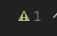
\includegraphics[scale=0.6]{IMG/Pycharm-11.png}
\caption{\textit{Pycharm} - Les avertissements d'erreurs}
\end{center}
\end{figure}
\medskip

Exemple: 
\begin{lstlisting}[caption=Les annotations de type]
def affichage(nb: int) -> str:
    return f"Le résultat est {nb}"


def calcul(a: int, b: int) -> str:
    produit = a * b
    return affichage(produit)


print(calcul(5, 5))
\end{lstlisting}
\medskip

Il faut savoir qu'avec le langage \texttt{Python} indiquer le type de paramètres n'est pas obligatoire, contrairement à d'autres langages de programmation. Et par conséquent les annotations de type viennent apporter un éclairage quant aux valeurs des paramètres pour la personne amenée à lire le code.
\medskip

Les annotations de type de la fonction \texttt{calcul()} présentée ci-dessus peuvent être affichées comme suit :
\begin{verbatim}
    >>> def calcul(a: int, b: int) -> str:
    ...     produit = a * b
    ...     return affichage(produit)
    ... 
    >>> calcul.__annotations__
    {'a': <class 'int'>, 'b': <class 'int'>, 'return': <class 'str'>}
\end{verbatim}
\medskip

L'interprète \texttt{Python} crée un \textit{dictionnaire}\footnote{Nous aborderons la notion de \textit{dictionnaire} avec les \textit{collections} (Cf. page \pageref{les_dictionnaires}).} à partir des annotations et les affecte à un \textit{attribut}\footnote{La notion d'\textit{attribut} sera abordée dans la partie consacrée à la \textit{programmation objet} (Cf. page \pageref{POO}).} spécial de la fonction appelé \texttt{\_\_annotations\_\_}. Les \textit{clés}\footnote{Les \textit{clés} seront vues avec la notion de \textit{dictionnaire}.} des paramètres sont les noms des paramètres. La clé de la valeur de retour est la chaîne de caractères \texttt{return}. Finalement, les annotations de type ne sont rien d'autre que des dictionnaires de métadonnées.
\medskip

\subsection*{La fonction \texttt{Annoted} du module \texttt{typing} : }
Depuis la version \texttt{3.9} de \texttt{Python}\footnote{Cf. PEP 593 – Flexible function and variable annotations - \url{https://peps.python.org/pep-0593/}} les annotations de type se sont vues améliorées, par l'ajout d'un contenu informationnel plus libre. Pour cela nous allons faire appel à la fonction \texttt{Annoted} du module \texttt{typing}:
\begin{lstlisting}[caption=Import de la fonction \texttt{Annoted}]
from typing import Annoted
\end{lstlisting}
\medskip

Voici alors la syntaxe que nous utiliserons dans la définition de la fonction:
\begin{verbatim}
    def nom_fonction(var: Annoted[type, "information libre"])
\end{verbatim}
\medskip

Le \texttt{PEP 593} vient introduire un mécanisme afin d'étendre les annotations de type convenues précédemment avec le \texttt{PEP 484}\footnote{Cf. PEP 484 – Type Hints - \url{https://peps.python.org/pep-0484/}}, en y ajoutant des métadonnées variées, spécifiques au contexte. S'agissant des fonctions, cela vient en complément du \texttt{PEP 3107}\footnote{Cf. PEP 3107 – Function Annotations - \url{https://peps.python.org/pep-3107/}} relatif aux annotations des fonctions.
\medskip

Il est tout à fait possible d'utiliser des annotations imbriquées:
\begin{lstlisting}[caption=Les annotations imbriquées]
def ma_fonction(var: Annoted[list[int]]):
\end{lstlisting}
\medskip

Il est aussi possible de déterminer des constantes de type.
\medskip

Illustrons tout cela par un petit script permettant de calculer l'IMC d'un individu:
\begin{lstlisting}[caption=Exemple d'annotations de type avec la fonction \texttt{Annoted}]
from typing import Annotated

# Constantes de type
ANNOTE_POIDS = Annotated[float, "Kg"]


def imc(poids: ANNOTE_POIDS, taille: Annotated[float, "mètre"]) \ 
        -> float:
    """Calcul de l'imc."""
    return poids / (taille * taille)


print(imc(67.5, 1.75))

# Pour afficher les informations sur les annotations :
print(imc.__annotations__)
print(ANNOTE_POIDS)
\end{lstlisting}
\medskip

Le code peut rapidement s'alourdir, mais en même temps cela offre la possibilité de documenter son code, et la méthode \verb|.__annotations__| vient nous offrir une lisibilité complète concernant les paramètres et retour d'une fonction. Voyons la sortie console du script précédent:
\begin{verbatim}
    22.040816326530614
    {'poids': typing.Annotated[float, 'Kg'], 'taille': typing.Annotated[float, 
      'mètre'], 'return': <class 'float'>}
    typing.Annotated[float, 'Kg']
\end{verbatim}
\medskip

\section{Le débogage avec une fonction}
Plaçons un point d'arrêt à la ligne correspondant à l'appel de fonction, puis on exécute le code en mode débogage. Arrivé au point d'arrêt on clique sur \texttt{Step into} pour entrer dans la fonction.
\begin{figure}[h]
\begin{center}
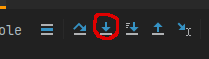
\includegraphics[scale=0.6]{IMG/Pycharm-09.png}
\caption{\textit{Pycharm} - Le bouton \texttt{Step into}}
\end{center}
\end{figure}
\medskip

On poursuit ensuite l'exécution ligne par ligne avec le bouton \texttt{Step Over}. Pour sortir le débogueur de la fonction afin de revenir au programme principal et poursuivre avec \texttt{Step Over} depuis le programme principal, on clique sur \texttt{Step Out}.
\begin{figure}[h]
\begin{center}
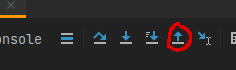
\includegraphics[scale=0.6]{IMG/Pycharm-10.png}
\caption{\textit{Pycharm} - Le bouton \texttt{Step Out}}
\end{center}
\end{figure}
\medskip

Sur \textit{Visual Studio Code} on emploie les boutons \texttt{Pas à pas détaillé} et \texttt{Pas à pas sortant}.
\begin{figure}[h]
\begin{center}

\includegraphics[scale=0.6]{IMG/VSC-04.png}
\caption{\textit{VSC} - Le bouton \texttt{Pas à pas détaillé}}
\end{center}
\end{figure}

\begin{figure}[h]
\begin{center}

\includegraphics[scale=0.6]{IMG/VSC-05.png}
\caption{\textit{VSC} - Le bouton \texttt{Pas à pas sortant}}
\end{center}
\end{figure}
\medskip

\section*{Sources utilisées pour la rédaction de ce chapitre}
\begin{itemize}
	\item[-] \textit{Comprendre les fonctions \texttt{Python}} - Thierry \textsc{Chappuis} - \textit{WePynaire} du 3 novembre 2022, disponible à l'adresse \url{https://edu.placepython.fr/}
	\item[-] \textit{Defining Your Own Python Function} (trad. \textit{Définir votre propre fonction \texttt{Python}} - John \textsc{Sturtz} - 9 mars 2020 - \url{https://realpython.com/defining-your-own-python}\\ \texttt{-function/} 
\end{itemize}
\medskip

\chapter{Les structures conditionnelles}\label{struct_cond}
\section{Condition et variable de type \og booléen\fg}
Voici le principe:
\begin{verbatim}
    Si condition:                 if condition:
        ...code...      ==>           ...code...
    Sinon:                        else:
        ...code...                    ...code...
\end{verbatim}
\medskip

\begin{lstlisting}[caption=Un premier exemple de structure conditionnelle]
  age = 8
  if age >= 18:
  	  print("Vous êtes majeur")
  else:
  	  print("Vous êtes mineur")
\end{lstlisting}
\medskip

Ce code affiche comme résultat:
\begin{verbatim}
    Vous êtes mineur
\end{verbatim}
\medskip

Les conditions retournent les valeurs \texttt{True} (\textit{Vrai}) et \texttt{False} (\textit{Faux}). Ce sont des valeurs dites \textit{booléennes} (\textit{boolean} en anglais).
\medskip

Voyons cela de façon plus explicite:
\begin{lstlisting}[caption=Les valeurs \textit{booléennes}]
  age = 8
  condition = age >= 18  # La condition est affectée à une variable
  if condition:  # Revient à dire: si condition == True
  	  print("Vous êtes majeur")
  else:  # Si condition == False
  	  print("Vous êtes mineur")
  print(condition)
  print(type(condition))
\end{lstlisting}
\medskip

Ce code nous retourne:
\begin{verbatim}
    Vous êtes mineur
    False
    <class 'bool'>
\end{verbatim}
\medskip

Le type de la variable \texttt{condition} est donc bien de type booléen.
\medskip

\section{Les opérateurs de comparaison}
Nous avons donc utilisé l'opérateur de comparaison \texttt{>=}, mais il existe en \textit{Python} huit opérateurs de comparaison.
\begin{table}[h]
\begin{center}
\begin{tabular}{|c|c|}
\hline
\textbf{Opérateur} & \textbf{Signification} \\
\hline
\texttt{<} & Strictement inférieur \\
\hline
\texttt{<=} & Inférieur ou égal \\
\hline
\texttt{>} & Strictement supérieur \\
\hline
\texttt{>=} & Supérieur ou égal \\
\hline
\texttt{==} & Égal \\
\hline
\texttt{!=} & Différent \\
\hline
\texttt{is} & Identité d'objet \\
\hline
\texttt{is not} & Contraire de l'identité d'objet \\
\hline 
\end{tabular}
\caption{Tableau des opérateurs de comparaison}
\end{center}
\end{table}
\medskip

Les opérateurs \texttt{is} et \texttt{is not} peuvent s'appliquer à deux objets quelconques. Ils ne retournent jamais d'exception.
\medskip

\section{La condition \texttt{elif}}
\texttt{elif} signifie \textit{sinon si...}, ce qui est la contraction de \textit{else if}. \texttt{elif} rend la condition exclusive, c'est-à-dire que si la condition est vraie les autres ne seront pas testées.
\begin{lstlisting}[caption=Sinon...si]
  if age == 17:
  	  print("Vous êtes presque majeur")
  elif age == 18:
  	  print("Tout juste majeur")
  elif age > 18:
  	  print("Vous êtes majeur")
  else:  # Exécuté si aucune des conditions d'avant n'est vrai
  	  print("Vous êtes mineur")
\end{lstlisting}
\medskip

Il peut y avoir autant de conditions \texttt{elif} que l'on en souhaite, cela fonctionne toujours comme un seul bloc de codes. L'ordre des conditions a son importance, ainsi que les formes conditionnelles, afin d'être sûr que toutes les conditions puissent être testées.
\medskip

Attention à ne pas commettre ce type d'erreur, qui ne plantera pas nécessaire l'exécution du code, mais qui amènerait à des incohérences dans son exécution:
\begin{verbatim}
    if condition:
        ...code...
    elif condition:
        ...code...
    if condition:
        ...code...
    else:
        ...code...
\end{verbatim}
\medskip

Cela fonctionne comme deux blocs de codes distincts: \texttt{if...elif} et \texttt{if...else}.
\medskip

\section{\texttt{and}/\texttt{or} (\textit{et}/\textit{ou})}
\begin{lstlisting}
  elif age >= 1 and age <= 2:
  	  print("Vous êtes encore un bébé")
\end{lstlisting}
\medskip

Une telle condition \texttt{elif} peut être modifiée de la façon suivante, dans la mesure où c'est la même variable qui est utilisée (ce qui est d'ailleurs recommandé):
\begin{lstlisting}
  elif 1 <= age <= 2:
\end{lstlisting}
\medskip

C'est ce que l'on appelle l'enchaînement de conditions. Ainsi:
\begin{verbatim}
    x < y <= z
\end{verbatim}
\medskip

C'est équivalent à:
\begin{verbatim}
    x < y and y <= z
\end{verbatim}
\medskip

\texttt{y} n'est évalué qu'une seule fois, et \texttt{z} ne sera pas évalué si \texttt{x < y} est faux.
\medskip

Nous aurions pu aussi utiliser \texttt{or} (pour \textit{ou}):
\begin{lstlisting}
  elif age == 1 or age == 2:
\end{lstlisting}
\medskip

Utiliser \texttt{and} est intéressant quand dans notre condition nous voulons faire appel à deux variables différentes:
\begin{lstlisting}[caption=\texttt{and} avec deux variables différentes]
  age = 20
  taille = 2
  if age >= 18 and taille >= 2:
  	  print("Vous êtes majeur et grand")
\end{lstlisting}
\medskip

\section{La correspondance structurelle}\label{correspondance_structurelle}
La correspondance structurelle (ou \textit{Structural pattern matching} en anglais) est l'une des fonctionnalités les plus importantes introduites dans la version \texttt{3.10} de \texttt{Python}\footnote{Cf. PEP 634 – Structural Pattern Matching: Specification - \url{https://peps.python.org/pep-0634/}}. Le \texttt{switch case} est une fonctionnalité déjà existante dans la majorité des langages de programmation, avec la version \texttt{3.10} elle fait donc son apparition dans le langage \texttt{Python}, sous le nom de \texttt{match case}. Désormais, avec \texttt{Python} nous pouvons réaliser de puissantes correspondances structurelles.
\medskip

Illustrons cela par un exemple simple à comprendre:
\begin{lstlisting}
while True:
    print("Choisir un nombre entre 1 et 5...(0 pour quitter)")
    choix = input("Votre choix : ")
    match choix:
        case "1" | "3" | "5":  # '|' pour 'or'
            print(f"{choix} est un chiffre impair")
        case "2" | "4":
            print(f"{choix} est un chiffre pair")
        case "0":
            break
        case _:  # Tous les autres cas
            print("Vous n'avez pas saisi le bon chiffre")
\end{lstlisting}
\medskip

La correspondance structurelle de type \texttt{match case} offre un code beaucoup plus concis que l'utilisation d'une structure conditionnelle avec des \texttt{if...else...}. Et avec un métacaractère (\textit{wild card} en anglais) comme l'underscore nous allons prendre en considération tous les autres cas de figure. Une déclaration de correspondance ne peut avoir qu'un seul et unique bloc \texttt{case} irréfutable, et ils doit être systématiquement positionné en dernier.
\medskip

Avec le \texttt{match case} nous allons aussi pouvoir tester la structure des données\footnote{Nous allons ici utiliser des dictionnaires, notion que nous aborderons plus loin avec les collections (page \pageref{collections}), mais j'estime qu'ici l'exemple est aisément compréhensible.}.
\begin{lstlisting}
# Divers dictionnaires avec des structures de données différentes :
auteur1 = {"nom": "DJIAN", "titre": "Sotos"}
auteur2 = {"nom": "KEROUAC", "livre": ("Sur la route", 1957)}
auteur3 = {"nom": "HEMINGWAY"}
auteur4 = {"titre": "Paris est une fête"}
auteur5 = {"nom": "DJIAN", "livre": ("Bleu comme l'enfer", 1981)}
auteur6 = {"nom": "BAUDELAIRE", "livre": ("Fleurs du Mal", 1857)}

auteurs = (auteur1, auteur2, auteur3, auteur4, auteur5, auteur6)

for auteur in auteurs:
    match auteur:
        case {"nom": nom, "livre": (titre, date_pub)} \
              if date_pub > 1900:
            print(f"{nom} a écrit {titre}, publié en {date_pub}.")
        case {"nom": nom, "livre": (titre, date_pub)}:
            print(f"{nom} a écrit {titre}, publié avant le "
                  f"XXe siècle")
        case {"nom": nom, "titre": titre}:
            print(f"{nom} a écrit {titre}.")
        case _:
            print(f"Aucune information exploitable pour {auteur}")
\end{lstlisting}
\medskip

Il faut toutefois être vigilant à l'ordre des \texttt{case} et insérer les cas les plus particuliers au début.
\medskip

Les mots clés \texttt{match} et \texttt{case} ne sont pas des mots réservés. Cela implique qu'ils ne sont reconnus comme tels que lorsqu'ils font partie d'un bloc \texttt{match}/\texttt{case}, en ayant bien les deux points à l'endroit prévu.
\medskip

\chapter{La boucle \texttt{for}}
Elle permet de boucle un certain nombre de fois ou sur un certain nombre d'éléments (nous verrons cela avec les séquences).
\medskip

\begin{verbatim}
    for i in range(0, 5):
\end{verbatim}
\medskip

\texttt{i} représente une variable. \textit{i} est utilisé par convention pour signifier \textit{index}. Une telle ligne de code pourrait se traduire ainsi: pour \texttt{i} de 0 à 5 (\texttt{range} pour \textit{ensemble}) on va boucler. Exemple de code fonctionnel:
\begin{lstlisting}[caption=Un premier exemple avec une boucle \texttt{for}]
  for i in range(0, 5):
  	  print(i)
\end{lstlisting}
\medskip

Cela donne en sortie:
\begin{verbatim}
    0
    1
    2
    3
    4
\end{verbatim}
\medskip

L'ensemble \texttt{range(0, 5)} est inclusif pour la première valeur (\texttt{0}) et exclusif pour la seconde (\texttt{5}). En expression mathématique cela donnerait l'ensemble \texttt{[0,5[}. En atteignant \texttt{5} (quand \texttt{i} vaut \texttt{5}) on va sortir de la boucle sans en exécuter le code qui suit.
\medskip

Imaginons un code qui vienne demander le nom de plusieurs personnes, où chacun d'entre elles viendrait alors saisir son nom:
\begin{lstlisting}[caption=Demander trois fois le nom]
  nbre_personnes = 3
  for i in range(0, nbre_personnes):
  	  nom = input("Quel est votre nom ? ")
  	  print("Bonjour " + nom)
\end{lstlisting}
\medskip

En sortie nous pourrions avoir:
\begin{verbatim}
    Quel est votre nom ? Paul
    Bonjour Paul
    Quel est votre nom ? Mattéo
    Bonjour Mattéo
    Quel est votre nom ? Loreleï
    Bonjour Loreleï
\end{verbatim}
\medskip

Idée de codage: imaginons demander à l'utilisateur non pas son livre préféré, mais ses trois livres préférés...
\medskip

%%%%%%%%%%%%%%%%%%%
%%% Chapitre 11 %%%
%%%%%%%%%%%%%%%%%%%
\chapter{Les affichages}
\section{Les chaînes formatées}
Au lieu de concaténer plusieurs chaînes de caractères on va faire appel au formatage qui permet de n'avoir qu'une seule et même chaîne de caractères. Ainsi, au lieu de coder:
\begin{verbatim}
    print("Vous vous appelez " + nom + ", vous avez " + str(age) + " ans.")
\end{verbatim}
\medskip

Nous pouvons coder:
\begin{verbatim}
    print(f"Vous vous appelez {nom}, vous avez {age} ans.")
\end{verbatim}
\medskip

Un autre formatage possible avec l'utilisation de \texttt{\%s}. Les paramètres à afficher ne sont plus les noms des variables, mais on leur substitut \texttt{\%s}, et les noms de variables sont insérés à la fin de la chaîne dans l'ordre voulu. Il s'agit de l'ancienne méthode de formatage de chaînes en \textit{Python}, qui est toujours valable.
\begin{verbatim}
    print("Vous vous appelez %s, vous avez %s ans." % (nom, age))
\end{verbatim}
\medskip

S'il y a plusieurs paramètres à insérer, ils doivent être placés entre parenthèses juste après le symbole \texttt{\%} et séparés par une virgule. A noter qu'avec les deux dernières méthodes une valeur de type numérique est automatiquement convertie en une valeur de type \textit{string}.
\medskip

Il n'y a pas selon moi de méthode mieux qu'une autre, chacun préférant la sienne. Pour ma part je trouve la deuxième méthode plus lisible. Ce sera donc celle-ci que j'utiliserai par la suite.
\medskip

\section{\texttt{print()} sur plusieurs lignes}
\begin{lstlisting}
  print("""Voici
  votre texte
  sur plusieurs
  lignes""")
\end{lstlisting}
\medskip

Ce qui donne en sortie:
\begin{verbatim}
    Voici
    votre texte
    sur plusieurs
    lignes
\end{verbatim}
\medskip

\section{Ajout de paramètres à la fonction \texttt{print()}}
\begin{lstlisting}
  nom = "Krystof"
  depart = 64
  print("Je m'appelle", nom, ". Je réside dasn le", depart)
\end{lstlisting}
\medskip

Ce qui donne en sortie:
\begin{verbatim}
    Je m'appelle Krystof . Je réside dans le 64
\end{verbatim}
\medskip

Chaque paramètre est suivi d'une espace, et les paramètres qui ne sont pas de type \textit{string} sont considérés comme tel automatiquement.
\medskip

\section{\texttt{lower()} et \texttt{upper()}}
\begin{verbatim}
    print("Krystof".lower())  # Affiche 'krystof' (minuscules)
    print("Krystof".upper())  # Affiche 'KRYSTOF' (majuscules)
\end{verbatim}
\medskip

\chapter{Les collections d'objets}\label{collections}
On va aborder ici des notions importantes de la programmation avec les collections qui nous permettent de contenir et gérer plusieurs éléments et ainsi optimiser notre code dans la manipulation de ces derniers (objets, variables). A cet effet \textit{Python} dispose des listes et \textit{tuples}, qui sont des objets fréquemment utilisés, et des dictionnaires et des sets.
\medskip

Ici nous aborderons les notions essentielles liées à ces objets, et nous approfondirons par la suite dans un chapitre dédiée en deuxième partie.
\medskip

\section{Les \textit{tuples}}
\subsection*{Présentation}
Syntaxe d'un \textit{tuple} (on utilise des parenthèses):
\begin{verbatim}
    mon_tuple = (var1, var2, var3)
\end{verbatim}
\medskip

Un \textit{tuple} n'est accessible, une fois créé, qu'en lecture seule, on ne peut donc le modifier. Il est dit \textit{immutable} (terme de programmation). Une liste (cf. section suivante), par contre, est elle \textit{mutable}.
\medskip

Illustrons le fonctionnement d'un \textit{tuple}:
\begin{verbatim}
    auteurs = ("Djian", "Kerouac", "Hemingway")
    print(auteurs)
\end{verbatim}
\medskip

Ce qui a pour effet d'afficher:
\begin{verbatim}
    ('Djian', 'Kerouac', 'Hemingway')
\end{verbatim}
\medskip

\subsection*{La notion d'indice}
Il est cependant possible de n'afficher qu'un seul élément à l'aide de ce que l'on nomme des indices:
\begin{verbatim}
    print(auteurs[0])
    print(auteurs[2])
    print(auteurs[3])
\end{verbatim}
\medskip

Respectivement, nous obtenons les sorties suivantes:
\begin{verbatim}
    Djian
    Hemingway
\end{verbatim}
\medskip

Mais pour le troisième \texttt{print()}, nous levons une exception de type \texttt{IndexError} avec la précision: \texttt{tuple index out of range}, que l'on peur traduire par \textit{au-delà de l'index}. Notons que l'indice \texttt{0} correspond au premier élément, et l'indice \texttt{2} au troisième. En fait les indices débutent à \texttt{0}, d'où le décalage. Dans notre exemple il y a trois éléments dans le \textit{tuple} \texttt{auteurs}. Ce que nous permet de vérifier l'instruction suivante:
\begin{verbatim}
    print(len(auteurs))
\end{verbatim}
\medskip

La sortie pour cette instruction est bien 3.
\medskip

Grâce aux indices nous allons ainsi pouvoir boucler sur notre objet de type \textit{tuple}:
\begin{verbatim}
    for i in range(0, len(auteurs)):
        print(auteurs[i]
\end{verbatim}
\medskip

Chaque élément de notre \textit{tuple} sera alors affiché:
\begin{verbatim}
    Djian
    Kerouac
    Hemingway
\end{verbatim}
\medskip

Une singularité du langage \textit{Python} réside dans la possibilité d'utiliser des indices inversés (indices négatifs). \texttt{print(auteurs[-1])} affiche en sortie: \texttt{Hemingway}. Avec un indice \texttt{-1} nous avons accès au dernier élément, avec \texttt{-2} à l'avant dernier élément, et ainsi de suite.
\medskip

Il est cependant possible de boucler sans l'aide des indices:
\begin{verbatim}
    for i in auteurs:
        print(i)
\end{verbatim}
\medskip

Nous venons ainsi d'itérer sur chaque élément du \textit{tuple}.

\subsection*{Similitudes avec ce que nous connaissons déjà}
Une chaîne de caractères se comporte comme un \textit{tuple}. Nous pouvons alors accéder aux divers éléments de la chaîne de caractères en bouclant sur cette dernière, avec ou sans indice.
\medskip

Avec la fonction \texttt{range()} nous obtenons des objets de type collection que nous pouvons apparenter à des \textit{tuples}:
\begin{verbatim}
    a = range(0, 5)
    print(a[-1])
\end{verbatim}
\medskip

Ce qui affiche \texttt{4} en sortie. En fait c'est comme si nous avions le \textit{tuple} suivant: \texttt{(0, 1, 2, 3, 4)}, objet sur lequel nous pouvons itérer et avec lequel nous pouvons utiliser des indices.
\medskip

\section{Les listes}
\subsection*{Présentation}
La syntaxe d'une liste est quasi similaire à celle d'un \textit{tuple}, sauf que l'on utilise des crochets au lieu de parenthèses.
\begin{verbatim}
    ma_liste = [var1, var2, var3]
\end{verbatim}
\medskip

Avec les listes nous pouvons réaliser ce que nous venons de voir avec les \textit{tuples}, mais également des manipulations supplémentaires. La différence entre ces deux types d'objets conteneurs est que les \textit{tuples} utilisent moins de mémoire que les listes, et que ces dernières peuvent par contre être modifiées.
\medskip

\subsection*{Modifier une liste}
Les listes sont des conteneurs, et les valeurs contenues dans ce conteneur sont modifiables. Voyons cela en ajoutant un élément à une liste:
\begin{verbatim}
    auteurs = ["Djian", "Kerouac", "Hemingway"]
    new_auteur = "Ravalec"
    auteurs.append(new_auteur)
    print(auteurs)
\end{verbatim}
\medskip

Et notre liste ainsi modifiée s'affiche ainsi:
\begin{verbatim}
    ['Djian', 'Kerouac', 'Hemingway', 'Ravalec']  
\end{verbatim}
\medskip

Supprimons maintenant l'élément situé à l'index \texttt{1}:
\begin{verbatim}
    del auteurs[1]
    print(auteurs)
\end{verbatim}
\medskip

Notre nouvelle liste affichée est alors la suivante:
\begin{verbatim}
    ['Djian', 'Hemingway', 'Ravalec']
\end{verbatim}
\medskip

Il est, bien évidemment envisageable de boucler sur les listes, à l'instar des \textit{tuples}.
\medskip

\subsection*{Petit exemple d'algorithme}
\begin{lstlisting}
    """LISTES - ALGO : Valeur la plus petite
    Détécter la valeur la plus petite et l'afficher en sortie,
    à l'aide des indices.
    Ici : afficher un nom à cette valeur minimale. """


    noms_chauffeurs_km = [("Patrick", 1.5), ("Paul", 2.2), 
                          ("Marc", 0.4), ("Jean", 0.9), 
                          ("Pierre", 7.1), ("Marie", 1.1),
                          ("Maxime", 0.6)]
    # Première distance comme valeur de référence:
    distance_min_et_nom = noms_chauffeurs_km[0]  

    for nom_et_distance in noms_chauffeurs_km:
        if nom_et_distance[1] < distance_min_et_nom[1]:
            distance_min_et_nom = nom_et_distance

    print(f"Distance minimale:{distance_min_et_nom[1]} km. "
          f"- Nom du chauffeur: {distance_min_et_nom[0]}.")
\end{lstlisting}
\medskip

\subsection*{Listes et fonction}
Voyons un exemple:
\begin{lstlisting}
    def modifier_valeur(a):
        a[0] = 10
    
    
    test = [1, 2, 3, 4]
    print(test)
    modifier_valeur(test)
    print(test)
\end{lstlisting}
\medskip

La sortie de ce code est:
\begin{verbatim}
    [1, 2, 3, 4]
    [10, 2, 3, 4]
\end{verbatim}
\medskip

\section{\textit{tuples} et fonction}
A l'aide des \textit{tuples} nous pouvons coder des fonctions qui retournent plusieurs valeurs, justement en retournant un \textit{tuple}. Pour cela on va utiliser l'instruction \texttt{return} et des virgules.
\begin{verbatim}
    return val1, val2, val3
\end{verbatim}
\medskip

Exemple:
\begin{lstlisting}
    def mon_tuple():
        return "Djian", "Kerouac", "Hemingway"
    
    
    # Affecter chaque valeur à une variable
    auteur1, auteur2, auteur3 = mon_tuple()
    # Ou créer un tuple:
    mes_auteurs = mon_tuple()
\end{lstlisting}
\medskip

Passer un \textit{tuple} à une fonction en séparant les valeurs:
\begin{lstlisting}
    def afficher(nom1, nom2, nom3):
        print(nom1)
        print(nom2)
        print(nom3)
    
    
    mes_auteurs = ("Djian", "Kerouac", "Hemingway")
    afficher(*mes_auteurs)  # Avec l'astérisque (*) on dit que l'on 
                            # unpack le tuple
    print(mes_auteurs)
    print(*mes_auteurs)  # Comme si on passait trois paramètres à la 
                         # fonction print()
\end{lstlisting}
\medskip

Ce code nous donne la sortie suivante:
\begin{verbatim}
    Djian
    Kerouac 
    Hemingway
    ('Djian', 'Kerouac', 'Hemingway')
    Djian Kerouac Hemingway
\end{verbatim}
\medskip

\section{Les \textit{slices}}
Les \textit{slices} sont des utilisations étendues des indices que l'on applique aux listes et aux \textit{tuples}. Syntaxe d'un \textit{slice}:
\begin{verbatim}
    [start:stop:step]
    ou
    [début:fin(exclue):pas]
\end{verbatim}
\medskip

Voici quelques exemples:
\begin{itemize}
	\item[[:]] -> l'ensemble de la liste;
	\item[[::2]] -> un élément sur deux (car avance de deux en deux dans la liste);
	\item[[::-1]] -> suit la liste dans l'ordre inversé;
	\item[[::-2]] -> Idem mais avec un élément sur deux.
\end{itemize}
\medskip

Les \textit{slices} s'appliquent aussi sur les chaînes de caractères.
\begin{verbatim}
    nom = "krystof"
    print(nom[1:3])  # Affiche 'ry'
    print(nom[::-1]  # Affiche 'fotsyrk'
\end{verbatim}
\medskip

\section{La fonction \texttt{sort()}}
\begin{verbatim}
    ma_liste.sort()
\end{verbatim}
\medskip

Le tri de la liste s'opère directement sur la liste elle-même en suivant l'ordre alphabétique de la table \texttt{ASCII}, autrement dit de \texttt{A} à \texttt{Z}, puis de \texttt{a} à \texttt{z}.
\medskip

Il est possible de modifier le comportement de la fonction \texttt{sort()}, et ce de deux façons:
\begin{verbatim}
    ma_liste.sort(reverse=True)  # Opère un tri inverse
    ma_liste.sort(key=mon_tri_personnalise)  # mon_tri_personnalise est une 
                                             # fonction dans laquelle on code 
                                             # le tri souhaité
\end{verbatim}
\medskip

\section{Les dictionnaires}\label{les_dictionnaires}
Le dictionnaire permet de structurer des données avec des champs, et par conséquent d'améliorer l'efficacité des certains algorithmes. Syntaxe d'un dictionnaire:
\begin{verbatim}
    mon_dico = {"cle":val1, "cle2":val2, "cle3":val3}
\end{verbatim}
\medskip

\subsection*{L'utilisation des dictionnaires}\label{utilisation_dict}
\begin{lstlisting}
pers = {'nom': 'jack', 'age': 25, 'taille': 1.60}
print(pers)
\end{lstlisting}
\medskip

Cela donne en sortie:
\begin{verbatim}
   {'nom': 'jack', 'age': 25, 'taille': 1.60} 
\end{verbatim}
\medskip

Nous pouvons sélectionner uniquement certains champs:
\begin{lstlisting}
print(pers['nom'])
\end{lstlisting}
\medskip

Le résultat est:
\begin{verbatim}
    jack
\end{verbatim}
\medskip

Un dictionnaire est mutable, nous pouvons donc lui réattribuer des valeurs.
\begin{lstlisting}
pers['nom'] = 'Ernest'
\end{lstlisting}
\medskip

Ou bien, depuis la version \texttt{3.9} de \texttt{Python}, à l'aide du \og \textit{pipe}\fg{} ('\texttt{|}'):
\begin{lstlisting}
pers|['nom', 'Ernest']
\end{lstlisting}
\medskip

Nous pouvons ajouter de nouvelles clés dynamiquement:
\begin{lstlisting}
pers['poste'] = "Développeur"
\end{lstlisting}
\medskip

Les dictionnaires peuvent contenir tout type de données: \texttt{str}, \texttt{int}, \texttt{float}, \textit{tuples}, listes, etc.
\medskip

Boucler sur un dictionnaire:
\begin{lstlisting}
for i in pers:
    print(i)
\end{lstlisting}
\medskip

Cela permet de récupérer l'ensemble des clés du dictionnaire:
\begin{verbatim}
    nom
    age
    taille
    poste
\end{verbatim}
\medskip

Pour afficher les valeurs, le code est:
\begin{lstlisting}
for i in pers:
    print(pers[i])
\end{lstlisting}
\medskip

Ainsi, pour récupérer l'intégralité du dictionnaire:
\begin{lstlisting}
for i in pers:
    print(f"clef: {i} - valeur: {pers[i]}")
\end{lstlisting}
\medskip

\subsection*{Fusion de deux dictionnaires}\label{fusion_dict}
Il existe la méthode du déballage, grâce à l'emploi des astérisques ('\texttt{*}'), mais il faut avouer que cela n'est pas très intuitif.
\begin{lstlisting}
dict1 = {"Jean": (20, "Développeur"), "Pierre": (30, "Ingénieur")}
dict2 = {"Émilie": (30, "Professeur"), "Marc": (25, "Chercheur")}

repertoire_complet = {**dict1, **dict2}
print(repertoire_complet)
\end{lstlisting}
\medskip

Ce qui nous donne en sortie :
\begin{verbatim}
    {'Jean': (20, 'Développeur'), 'Pierre': (30, 'Ingénieur'), 'Émilie': (30, 
    'Professeur'), 'Marc': (35, 'Chercheur')}
\end{verbatim}
\medskip

Il est possible d'utiliser la méthode du déballage de la façon suivante:
\begin{lstlisting}
repertoire_complet = dict(dict1, **dict2)
\end{lstlisting}
\medskip

A noter toutefois, que cette dernière méthode ne fonctionne que si \texttt{dict2} n'utilise que des clés de type \texttt{str}.
\medskip

Pour un même résultat, mais avec l'emploi de la méthode \texttt{update()}, nous avons:
\begin{lstlisting}
dict1.update(dict2)
\end{lstlisting}
\medskip

Avec cette méthode, on ajoute \texttt{dict1} à \texttt{dict2}, ce qui finalement va écraser le \texttt{dict1} initial. De plus, avec des dictionnaires volumineux une telle opération va nécessité beaucoup de capacité mémoire.
\medskip

Depuis la version \texttt{3.9} de \texttt{Python}\footnote{Cf. PEP 584 – Add Union Operators To dict - \url{https://peps.python.org/pep-0584/}}. nous pouvons recourir à l'utilisation de l'opérateur \textit{pipe} ('\texttt{|}'), qui permet la concaténation.
\begin{lstlisting}
dict_complet = dict1 | dict2
\end{lstlisting}
\medskip

Ou bien encore:
\begin{lstlisting}
dict1 |= dict2
\end{lstlisting}
\medskip

Il s'agit d'une concaténation équivalente à \texttt{dict1 = dict1 + dict2}. C'est une affectation augmentée qui fonctionne \og \textit{in-place}\fg{}, et qui se trouve être beaucoup plus efficiente au niveau mémoire comparativement à la méthode \texttt{dict1.update(dict2)}.
\medskip

Avec toutes ces diverses méthodes, il faut savoir que les éventuels conflits de clés sont résolus, puisque seule la clé la plus à droite, autrement dit la dernière clé vue, sera prise en considération.
\medskip

En terme de performance, si l'on souhaite fusionner un grand nombre de dictionnaires, il est préférable d'utiliser une boucle explicite et une union dite \og \textit{in-place}\fg{}:
\begin{lstlisting}
new_dico = {}
for d in ensemble_dicos:
    new_dico |= d
\end{lstlisting}
\medskip
 
\subsection*{Liste \textit{vs} dictionnaire}
Avec une liste, pour rechercher un élément contenu dans la liste il va nous falloir itérer sur cette dernière. Avec le dictionnaire, grâce à la clé, nous avons un accès direct. Le dictionnaire va ainsi permettre une exécution plus rapide du programme, notamment si la masse de données est importante.
\medskip

\subsection*{Si la clé n'existe pas}
Quand la clé sollicitée n'existe par, \textit{Python} lève une exception de type \texttt{KeyError}. Pour gérer ce cas de figure la méthode \texttt{.get()} retourne la valeur \texttt{None}.
\begin{lstlisting}
habite = pers.get("ville")
if not habite:  # Equivalent à if habite == None:
	...code...
\end{lstlisting}
\medskip

%%%%%%%%%%%%%%%%%%%%%%%%
%%% Troisième partie %%%
%%%%%%%%%%%%%%%%%%%%%%%%
\part{\textcolor{cyan}{Devenons plus intime avec \textit{Python}: notions intermédiaires}}

\chapter{Notions approfondies concernant les chaînes de caractères}
\section{Préfixes et suffixes d'une chaîne de caractères}
\subsection*{La méthode \texttt{strip()}}
Par défaut la fonction \texttt{strip()} supprime les espaces situés en fin et en début de chaîne.
\begin{lstlisting}
p = "     ma chaîne    "
print(p.strip())
\end{lstlisting}
\medskip

Ce qui nous donne en sortie:
\begin{verbatim}
    ma chaîne
\end{verbatim}
\medskip

Avec un paramètre nous pouvons préciser ce qui doit être supprimer dans la chaîne:
\begin{lstlisting}
p = "ma chaîne"
print(p.strip("ma "))
\end{lstlisting}
\medskip

'\texttt{ma}' sera supprimé, et seul '\texttt{chaîne}' sera affiché. Mais cette méthode a ses limites.
\begin{lstlisting}
p = "ceci est ma chaîne"
print(p.srip("chaîne"))
\end{lstlisting}
\medskip

Cela aura pour effet d'afficher uniquement '\texttt{est ma}'. Cela s'explique par le fait que la fonction \texttt{strip()} va regarder au début de la chaîne et se centre sur '\texttt{ceci}'. '\texttt{c}' est dans '\texttt{chaîne}', alors on supprime '\texttt{c}'. Cela va fonctionner à l'identique pour les lettres '\texttt{e}', '\texttt{i}' et le second '\texttt{c}'. Puis la fonction \texttt{strip()} se centrera ensuite sur le mot '\texttt{chaîne}' afin de la supprimer.
\medskip

\subsection*{Les fonctions \texttt{removeprefix()} et \texttt{removesuffix()}}\label{prefix_suffix}
La version \texttt{3.9} de \texttt{python} introduit deux nouvelles fonctions\footnote{Cf. PEP 616 – String methods to remove prefixes and suffixes - \url{https://peps.python.org/pep-0616/}}.
\begin{lstlisting}
p = "ceci est ma chaine"
# Pour supprimer uniquement 'chaine':
print(p.removesuffix("chaine"))
# Pour supprimer uniquement 'ceci':
print(p.removeprefix("ceci"))
# Pour supprimer 'ceci' et 'chaine':
print(p.removeprefix("ceci").removesuffix("chaine"))
\end{lstlisting}
\medskip

\chapter{Notions approfondies concernant les fonctions}
\section{Nombre variable de paramètres}
Dans certains cas, lorsque vous définissez une fonction, vous ne savez pas à l'avance combien d'arguments vous souhaitez lui faire prendre. Mais, comme vous l'avez déjà vu, lorsque des arguments positionnels sont utilisés, le nombre d'arguments transmis doit correspondre au nombre de paramètres déclarés. Pour résoudre ce problème, nous faisons alors appel à l'empaquetage des arguments (\og \textit{Argument packing}\fg{}). Lorsqu'un nom de paramètre dans une définition de fonction \texttt{Python} est précédé d'un astérisque (\texttt{*}), cela indique que les tous les arguments correspondants dans l'appel de fonction sont empaquetés dans un \textit{tuple} auquel la fonction peut faire référence par le nom du paramètre donné. Voici un exemple :
\begin{lstlisting}[caption=Nombre de paramètres non connu]
def somme(*nbres):  
    # '*' pour signifier le nombre inconnu de paramètres
    resultat = 0
    for n in nbres:
        resultat += n
    return resultat
  
  
print(somme(5, 2, 4, 7, 8))  # Affiche 26
print(somme(5, 2, 4))  # Affiche 11
print(somme())  # Affiche 0
\end{lstlisting}
\medskip

Une opération analogue est disponible de l'autre côté de l'équation dans un appel de fonction \texttt{Python}. Lorsqu'un argument dans un appel de fonction est précédé d'un astérisque (\texttt{*}), cela indique que l'argument est un \textit{tuple} qui doit être décomposé et transmis à la fonction en tant que valeurs séparées :
\begin{lstlisting}[caption=Décomposition de \textit{tuple}]
def somme(a, b, c):
    resultat = a + b + c
    return resultat


tuple_de_nbres = (5, 6, 9)
print(somme(*tuple_de_nbres))
\end{lstlisting}
\medskip

L'opérateur astérisque (\texttt{*}) peut être appliqué à tout itérable dans un appel de fonction \texttt{Python}, comme par exemple une liste ou un ensemble.
\medskip

Vous pouvez même utiliser l'empaquetage et le dépaquetage de \textit{tuple} en même temps :
\begin{lstlisting}[caption=Empaquetage et dépaquetage]
def somme(*args):
    # '*' pour signifier le nombre inconnu de paramètres
    return sum(args)


a = (5, 6, 9)
b = (31, 54, 53, 5)
c = (3, 5, 86, 4, 4, 646, 42)
print(somme(*a))  # Affiche 20
print(somme(*b))  # Affiche 143
print(somme(*c))  # Affiche 790
\end{lstlisting}
\medskip

Peu importe le nom donné au paramètre, ce qui importe c'est la présence de l'astérisque (\texttt{*}). Cependant, par convention (par usage) c'est le mot \texttt{args} qui sera donné au paramètre, ainsi la fonction sera définie de la façon suivante:
\begin{verbatim}
    def nom_fonction(*args)
\end{verbatim}
\medskip

\texttt{Python} dispose d'un opérateur similaire, le double astérisque (\texttt{**}), qui peut être utilisé avec les paramètres et les arguments des fonctions pour spécifier l'empaquetage et le dépaquetage des dictionnaires. Faire précéder un paramètre d'un double astérisque (\texttt{**}) dans une définition de fonction indique que les arguments correspondants, qui sont censés être des paires \texttt{clé=valeur}, doivent être empaquetés dans un dictionnaire :
\begin{lstlisting}[caption=Paramètres avec clé associée]
def moyenne(**nbres):
    # '**' pour signifier des paramètres avec clé associée
    somme = 0
    for n in nbres.values():
        # Pour récupérer les valeurs associées à une clé
        somme += n
    return round(somme / len(nbres), 2)


print(f"Moyenne des notes : "
      f"{moyenne(maths=15, geo=11, anglais=18)}")
\end{lstlisting}
\medskip

Ce code donne en sortie:
\begin{verbatim}
    Moyenne des notes : 14.67
\end{verbatim}
\medskip

Dans cet exemple, les arguments \texttt{maths=15, geo=11, anglais=18} sont empaquetés dans un dictionnaire que la fonction peut référencer par le nom \texttt{kwargs}. Encore une fois, n'importe quel nom peut être utilisé, mais le nom particulier \texttt{kwargs} (qui est l'abréviation de \og \textit{keyword args}\fg{}) est presque standard. Vous n'êtes pas obligé de l'utiliser, mais si vous le faites, toute personne connaissant les conventions de codage \texttt{Python} saura immédiatement ce que vous voulez dire.
\medskip

Le dépaquetage d'un dictionnaire d'arguments est analogue au dépaquetage d'un \textit{tuple} d'arguments. Lorsque le double astérisque (\texttt{**}) précède un argument dans un appel de fonction \texttt{Python}, il indique que l'argument est un dictionnaire qui doit être décomposé, et que les éléments résultants sont passés à la fonction en tant qu'arguments avec mots-clés :
\begin{lstlisting}[caption=Dépaquetage d'un dictionnaire]
notes = {"maths": 15, "geo": 11, "anglais": 18}
print(f"Moyenne des notes : {moyenne(**notes)}")
\end{lstlisting}
\medskip

Les éléments du dictionnaire \texttt{notes} sont décompressés et passés à la fonction \texttt{moyenne()} comme arguments avec mots-clés. Ainsi, \texttt{moyenne(**notes)} est équivalent à \texttt{moyenne(maths=15, geo=11, anglais=18)}.
\medskip

Les trois paramètres positionnels (standard, \texttt{*args} et \texttt{**kwargs}) peuvent être utilisés ensemble dans une définition de fonction \texttt{Python}. Si tel est le cas, ils doivent être spécifiés dans cet ordre :
\begin{verbatim}
    def nom_fonction(standard, *args, **kwargs):
\end{verbatim}
\medskip

Voici un exemple:
\begin{lstlisting}[caption=Paramètres mixées]
def creer_liste(num_liste, *elements, **options):
    # '*' pour grouper les paramètres (capture les arguments 
    # surnuméraires).
    # '**' pour grouper les arguments par mots clés.
    ma_liste = []
    print("-" * 10)
    print(f"Liste {num_liste} : ")
    print(f"elements = {type(elements)}")  # Affiche le tuple.
    print(f"options = {type(options)}")  # Le dictionnaire.
    for element in elements:
        if options.get("upper"):
            element = element.upper()
        elif options.get("capitale"):
            element = element.capitalize()
        ma_liste.append(element)
    print(f"Les paramètres optionels = {options}")
    return ma_liste  # Avec retour d'objet


def affichage_liste(*listes):
    num_liste = 1
    for liste in listes:
        print(f"Liste {num_liste}: {liste}")
        num_liste += 1


# Appels de fonction :
liste_mots = creer_liste(1, 'livre', 'bibliothèque', 'marque_page',
                         option1=100, option2=200)
liste_noms_auteurs = creer_liste(2, "kerouac", "djian", "hemingway",
                                 upper=True)
liste_nom_modifiee = creer_liste(3, "kerouac", "djian", "hemingway",
                                 upper=False)
liste_prenoms_auteurs = creer_liste(4, "jack", "philippe", "ernest",
                                    capitale=True)
# Affichages des listes à l'aide d'une autre fonction :
print("-" * 10)
affichage_liste(liste_mots, liste_noms_auteurs,
                liste_nom_modifiee, liste_prenoms_auteurs)
\end{lstlisting}
\medskip

Ce qui donne en sortie:
\begin{verbatim}
    ----------
    Liste 1 : 
    elements = <class 'tuple'>
    options = <class 'dict'>
    Les paramètres optionels = {'option1': 100, 'option2': 200}
    ----------
    Liste 2 : 
    elements = <class 'tuple'>
    options = <class 'dict'>
    Les paramètres optionels = {'upper': True}
    ----------
    Liste 3 : 
    elements = <class 'tuple'>
    options = <class 'dict'>
    Les paramètres optionels = {'upper': False}
    ----------
    Liste 4 : 
    elements = <class 'tuple'>
    options = <class 'dict'>
    Les paramètres optionels = {'capitale': True}
    ----------
    Liste 1: ['livre', 'bibliothèque', 'marque_page']
    Liste 2: ['KEROUAC', 'DJIAN', 'HEMINGWAY']
    Liste 3: ['kerouac', 'djian', 'hemingway']
    Liste 4: ['Jack', 'Philippe', 'Ernest']   
\end{verbatim}
\medskip

Cela offre à peu près toute la flexibilité dont vous pourriez avoir besoin dans une \textit{interface de fonction}.
\medskip

La version \texttt{3.5} de \texttt{Python} a introduit le \textit{dépaquetage multiple} dans un appel de fonction, comme indiqué dans le \texttt{PEP 448}\footnote{\texttt{PEP 448} – \textit{Additional Unpacking Generalizations} (trad. \og \textit{Généralités supplémentaires sur le déballage}\fg{}) - \url{https://peps.python.org/pep-0448/}}. Une telle amélioration permet notamment de réaliser plusieurs dépaquetages dans un seul appel de fonction :
\begin{lstlisting}[caption=Dépaquetage multiple]
def ma_fonction(**kwargs):
    for k, v in kwargs.items():
        print(k, '->', v)


d1 = {'a': 1, 'b': 2}
d2 = {'x': 3, 'y': 4}
ma_fonction(**d1, **d2)
\end{lstlisting}
\medskip

Ce qui nous donne en sortie:
\begin{verbatim}
    a -> 1
    b -> 2
    x -> 3
    y -> 4
\end{verbatim}
\medskip

\section{Les fonctions récursives}
Les fonctions récursives sont des fonctions qui peuvent être rappelées par elles-mêmes, mais il faut demeurer vigilant au fait qu'elles aient toujours une condition de sortie, au risque de se retrouver avec une boucle infinie.
\begin{lstlisting}[caption=Exemple de boucle sans fin]
  def f(nbre):
    print(nbre)
    f(nbre)


  f(2)  # Affichage du nombre 2 à l'infini
\end{lstlisting}
\medskip
 
Voyons maintenant une vraie fonction récursive:
\begin{lstlisting}[caption=Fonction récursive]
  def f(nbre, limite):
    if nbre > limite:
        return
    print(nbre)
    f(nbre*nbre, limite)
  
  
  f(2, 1000)
\end{lstlisting}
\medskip

Ce qui donne en sortie:
\begin{verbatim}
    2
    4
    16
    256
    65536
\end{verbatim}
\medskip

\section{Différence entre \texttt{break} et \texttt{return}}
\texttt{break} permet de sortir d'une boucle et \texttt{return} permet de sortir d'une fonction. \texttt{break} peut s'utiliser en dehors d'une fonction tandis que ce n'est pas le cas pour \texttt{return}.
\medskip

\section{Les fonctions \textit{callback} et \textit{lambda}}
\subsection*{Principe des fonctions \textit{callback}}
\begin{verbatim}
    a = ma_fonction
\end{verbatim}
\medskip

Sans les parenthèses, la fonction ne sera pas exécutée. La fonction est simplement affectée à une variable qui devient alors une référence à la fonction. Du coup, \verb|a()| est équivalent à \verb|ma_fonction()|. Le fait de passer une fonction à une variable est ce que l'on appelle le \textit{callback}.
\medskip

Exemple à tester:
\begin{lstlisting}[caption=Le \textit{callback}]
def afficher_table(n, operateur_str, operation_cbk):  
    # cbk = abréviation de callback
    for i in range(1, 10):
        print(f"{i} {operateur_str} {n} = "
              f"{operation_cbk(i, n)}")
  
  
def mult_cbk(a, b):
    return a*b


def add_cbk(a, b):
    return a+b


afficher_table(2, "x", mult_cbk)
print("-" * 10)
afficher_table(2, "+", add_cbk)
\end{lstlisting}
\medskip

\subsection*{Les fonctions \textit{lambda}}
Ce sont des fonctions qui n'ont pas de nom. Il s'agit de fonctions courtes qui ne contiennent que du code que l'on insère directement sans faire appel à la fonction (d'ailleurs impossible puisque la fonction n'a pas de nom).
\medskip

Ainsi la fonction \verb|mult_cbk()| vue précédemment pourrait s'écrire:
\begin{verbatim}
    lambda a,b : a*b
\end{verbatim}
\medskip

L'appel de la fonction \texttt{afficher\_table} peut donc au final s'écrire:
\begin{verbatim}
    afficher_table(2, "x", lambda a,b : a*b)
\end{verbatim}
\medskip

Il n'y a alors plus besoin de la fonction \texttt{mult\_cbk()}. Pareil avec la fonction \texttt{add\_cbk()} qui devient \texttt{lambda a,b : a+b}.
\medskip

Au final cela permet d'avoir du code très compact.
\medskip

\section{Les \textit{décorateurs}}
Un \textit{décorateur} va venir décorer une fonction. C'est en fait une fonction qui prend en paramètres une autre fonction. Ils vont nous permettre d'exécuter du code avant et après celui de la fonction qu'ils décorent.
\medskip

Illustrons cela par un script commenté:
\begin{lstlisting}[caption=Fonction avec décorateur]
from functools import wraps  # wraps nous permet de conserver 
# nom et documentation de la fonction décorée.


def mon_decorateur(une_fonction):
    @wraps(une_fonction)  # Au lieu des lignes 22 et 24
    def mon_decorateur_interne(*args, **kwargs):
        # *args pour tous les paramètres positionnés
        # et **kwargs pour les paramètres nommés.
        # Autrement nous pouvons juste utiliser les paramètres  
        # de la fonction qui doit être décorée.
        # 'args' et 'kwargs' sont des conventions Python de 
        # nommage.
        # Il est conseillé de mettre les deux, car on ne sait 
        # pas si nous aurons des arguments positionnels ou 
        # nommés.
        print("Code exécuté avant la fonction...")
        # Stockage de la variable décorée dans une variable :
        # Pour un retour direct nous aurions codé :
        # -> return une_fonction(*args, **kwargs)
        valeur = une_fonction(*args, **kwargs)
        print("Code exécuté après la fonction...")
        return valeur
    # Pour garder le nom de la fonction d'origine :
    #mon_decorateur_interne.__name__ = une_fonction.__name__
    # Pour garder la documentation de la fonction d'origine :
    #mon_decorateur_interne.__doc__ = une_fonction.__doc__
    return mon_decorateur_interne


@mon_decorateur  # C'est ainsi que l'on décor une fonction
# ==> Ceci est équivalent à :
# ma_fonction = mon_decorateur(une_fonction=ma_fonction)
def ma_fonction(a):
    """Documentation de ma fonction :
    Ici, se contente d'afficher un message."""
    print(f"Dans ma fonction{a} : ")
    print(f"a = {a}")


@mon_decorateur
def ma_fonction2(a, b):
    print(f"Dans ma fonction{b} :")
    print(f"a = {a} - b = {b}")


@mon_decorateur
def ma_fonction3(a, b, c):
    print(f"Dans ma fonction{c} :")
    print(f"a = {a} - b = {b} - c = {c}")


# Une fonction est affectée au décorateur et est retournée 
# via la variable :
# ma_fonction = mon_decorateur(une_fonction=ma_fonction)
ma_fonction(1)
print(f"print(ma_fonction) : {ma_fonction}")
print(f"ma_fonction.__name__ : {ma_fonction.__name__}")
print(f"ma_fonction.__doc__ : {ma_fonction.__doc__}")
print("-"*10)
ma_fonction2(1, 2)
print("-"*10)
ma_fonction3(1, 2, 3)
print("-"*10)
# Pour démontrer que le décorateur est bien une fonction :
print(f"La fonction 'mon_decorateur' : {mon_decorateur}")
\end{lstlisting}
\medskip

\section*{Sources utilisées pour la rédaction de ce chapitre}
\begin{itemize}
	\item[-] \textit{Comprendre les fonctions \texttt{Python}}, par Thierry \textsc{Chappuis} - \textit{WePynaire} du 3 novembre 2022, disponible à l'adresse \url{https://edu.placepython.fr/}
	\item[-] \textit{Defining Your Own Python Function} (trad. \og \textit{Définir votre propre fonction \texttt{Python}\fg{}}, par  John \textsc{Sturtz}, 9 mars 2020 - \url{https://realpython.com/defining-your-own-python-function/}
\end{itemize}
\medskip

%%%%%%%%%%%%%%
%%%    Chapitre 2    %%%
%%%%%%%%%%%%%%
\chapter{Notions approfondies concernant les collections}
\section{\texttt{append}, \texttt{extend}, \texttt{+=} et \texttt{insert}}
Créons quelques listes:
\begin{lstlisting}
auteurs = ["Djian", "Kerouac", "Marsé"]
poetes = ["Baudelaire", "Verlaine"]
classiques = ["Hugo", "Stendhal"]
philosophes = ["Morin", "Rousseau"]
auteurs2 = ["Ravalec", "McMurtry"]
\end{lstlisting}
\medskip

La méthode \texttt{.append()} ne permet d'insérer qu'un seul item:
\begin{lstlisting}
auteurs.append("Hemingway")
\end{lstlisting}
\medskip

Pour ajouter tous les éléments un à un d'autre liste, nous allons utiliser la boucle \texttt{for}:
\begin{lstlisting}
for e in poetes:
    auteurs.append(e)
\end{lstlisting}
\medskip

Ajouter tous les éléments d'une liste à une autre (deux méthodes):
\begin{lstlisting}
auteurs.extend(classiques)
#    ou
auteurs += classiques
\end{lstlisting}
\medskip

Insérer une nouvelle liste dans une liste à l'index souhaité. La nouvelle liste sera un élément de la liste:
\begin{lstlisting}
auteurs.insert(2, auteurs2)  # Insertion à l'index 2
\end{lstlisting}

Comme avec les chaînes de caractères il est possible d'utiliser la concaténation avec des listes:
\begin{lstlisting}
liste_complete_auteurs = auteurs + philosophes 
\end{lstlisting}
\medskip

Affichons maintenant tout cela:
\begin{lstlisting}
print(f"Ma liste d'auteurs {auteurs}")
print(f"\nMa liste d'auteurs complète {liste_complete_auteurs}")
\end{lstlisting}
\medskip

En sortie:
\begin{verbatim}
Ma liste d'auteurs ['Djian', 'Kerouac', ['Ravalec', 'McMurtry'], 'Marsé', 
'Hemingway', 'Baudelaire', 'Verlaine', 'Hugo', 'Stendhal']

Ma liste d'auteurs complète ['Djian', 'Kerouac', ['Ravalec', 'McMurtry'], 'Marsé', 
'Hemingway', 'Baudelaire', 'Verlaine', 'Hugo', 'Stendhal', 'Morin', 'Rousseau']
\end{verbatim}
\medskip

\section{Copier une liste \textit{vs} pointer sur une liste}
\begin{itemize}
	\item[\texttt{var = noms[:]}]: Va permettre une copie de la liste et l'affecter à la variable \texttt{var}. Une modification de la liste contenue dans \texttt{var} n'aura aucune incidence sur celle contenue dans \texttt{noms}, car en mémoire il y a deux listes distinctes.
	\item[\texttt{var = nom}]: Ici la variable \texttt{var} copie le nom de la variable \texttt{nom}. Toute modification de la liste par la variable \texttt{var} viendra modifier la liste affectée à la variable \texttt{nom}, car en fait \texttt{var} et \texttt{nom} pointent sur la même collection, il n'y a qu'une seule liste en mémoire.
\end{itemize}
\medskip

\section{Les tris: \texttt{sort()} \textit{vs} \texttt{sorted()}}
Trier une liste alphabétiquement:
\begin{lstlisting}
liste.sort()
\end{lstlisting}
\medskip

L'ordre des éléments est directement modifié au niveau de la liste. Aucune nouvelle liste n'est donc créée. On dit que l'opération est réalisée \og en place\fg{}.
\medskip

Pour créer une nouvelle liste on va utiliser la fonction \texttt{sorted()}:
\begin{lstlisting}
liste_triee = sorted(liste)
\end{lstlisting}
\medskip

Trier une liste dans l'ordre inverse de l'ordre alphabétique:
\begin{lstlisting}
liste.sort(reverse=True)
liste_triee = sorted(liste, reverse=True)
\end{lstlisting}
\medskip

Il est possible de réaliser des tris personnalisés à l'aide d'une fonction, et notamment une fonction \textit{lambda}. L'option \texttt{key}, qui appelle une fonction, va nous permettre cela. Voyons l'exemple d'une fonction qui opérerait un tri sur la longueur de chaque élément, en les triant du plus petit au plus grand:
\begin{lstlisting}
liste.sort(key=lambda x:len(x))
\end{lstlisting}
\medskip

\texttt{x} représente l'entrée de la fonction et \texttt{len(x)} la sortie. Tenant compte de la longueur de chaque élément de la liste mais en les classant du plus grand au plus petit, le code est:
\begin{lstlisting}
liste.sort(key=lambda x:len(x), reverse=True)
\end{lstlisting}
\medskip

Nous pouvons aussi définir une fonction est l'appeler avec l'option \texttt{key}. \texttt{key=nom\_fonction}: attention il n'y a pas les parenthèses d'appel.
\medskip

Le paramètre \texttt{key} s'utilise aussi avec la fonction \texttt{sorted()}.
\medskip

\section{Opérations sur les éléments d'une collection avec les fonctions \texttt{min()}, \texttt{max()}, \texttt{sum()} et l'opérateur \texttt{in}}
\begin{itemize}
	\item[\texttt{min(collection)}]: donne la valeur minimale;
	\item[\texttt{max(collection)}]: donne la valeur maximale
\end{itemize}
\medskip

Appliqué à une chaîne de caractères, \texttt{min()} va retourner le caractère situé le plus bas dans l'ordre alphabétique, et \texttt{max} le plus haut. Cependant ce n'est pas une pratique recommandée car cela ne donne pas nécessairement un code lisible.
\medskip

L'opérateur \texttt{in} permet de vérifier la présence d'un élément dans une collection. Est-ce que l'élément est contenu dans la liste:
\begin{lstlisting}
if element in liste:
\end{lstlisting}
\medskip

\texttt{sum(collection)}: calcule la somme de la collection, uniquement si les éléments de la collection sont des données de valeur numérique.
\medskip

\section{\textit{Swapper} deux éléments d'une liste}
Il s'agit ici d'échanger deux éléments d'une liste de façon atomique (c'est-à-dire en une seule ligne):
\begin{lstlisting}
liste[0], liste[4] = liste[4], liste[0]
\end{lstlisting}
\medskip

\section{\texttt{join} et \texttt{split}}
\begin{itemize}
	\item[\texttt{join}]: signifie \og rejoindre\fg{} et permet de coller ensemble les éléments de la collection;
	\item[\texttt{split}]: signifie \og séparer\fg{}. 
\end{itemize}
\medskip

Avec les fonctions \texttt{join()} et \texttt{split()} on va utiliser des séparateurs.
\begin{lstlisting}
mots = ["chat", "chien", "poule"]
mots_joints = "-".join(mots)
print(mots_joints)
\end{lstlisting}
\medskip

Ce qui donne en sortie:
\begin{verbatim}
    chat-chien-poule
\end{verbatim}
\medskip

A l'inverse:
\begin{lstlisting}
new_liste = mots_joints.split("-")
print(new_liste)
\end{lstlisting}
\medskip

La sortie est alors une nouvelle liste:
\begin{verbatim}
    ['chat', 'chien', 'poule']
\end{verbatim}
\medskip

\section{\texttt{index()}, \texttt{find()} et \texttt{count()}}
Pour obtenir l'index (indice) d'un élément dans une liste: \texttt{liste.index(element)}. Si l'élément recherché ne figure pas dans la liste, \textit{Python} lève une exception de type \texttt{ValueError}. Si la liste contient deux éléments de même valeur, c'est l'index de la première occurrence qui est donné.
\medskip

Il est toutefois possible de débuter la recherche de l'occurrence voulue à compter d'un index que l'on définit. Ainsi pour rechercher une occurrence à compter de l'index \texttt{3} (donc en ne tenant pas compte des éléments situés avant cet index): \texttt{liste.index(element, 3)}.
\medskip

\texttt{liste.count(element)}: donne le nombre d'occurrences (\texttt{element}) de même valeur.
\medskip

Illustrons cela par le code suivant:
\begin{lstlisting}
poetes = ["Baudelaire", "Verlaine", "Cros", "Verlaine",
          "Hugo", "Ronsard", "Verlaine"]

element_cherche = "Verlaine"
nb_occurences = poetes.count(element_cherche)
print(f"Nombre d'occurences pour '{element_cherche}': "
      f"{nb_occurences}")
      
if nb_occurences > 0:
    index_occurence = 0
    for i in range(nb_occurences):
        index_occurence = poetes.index(element_cherche, 
                                       index_occurence)
        print(f"'{element_cherche}' trouvé à l'index "
              f"{index_occurence}")
        index_occurence += 1
else:
    print(f" '{element_cherche}' n'est pas dans la liste")
\end{lstlisting}
\medskip

La sortie de ce code est:
\begin{verbatim}
    Nombre d'occurences pour 'Verlaine': 3
    'Verlaine' trouvé à l'index 1
    'Verlaine' trouvé à l'index 3
    'Verlaine' trouvé à l'index 6
\end{verbatim}
\medskip

\texttt{find()} ne fonctionne pas avec les collections mais peut s'utiliser avec des chaînes de caractères.
\begin{lstlisting}
a = "Baudelaire-Verlaine-Hugo"
i = a.find("Verlaine")
print(i)
\end{lstlisting}
\medskip

En sortie nous aurons le début de l'index pour \og \texttt{Verlaine}\fg{}:
\begin{verbatim}
    11
\end{verbatim}
\medskip

Si l'occurrence n'est pas trouvée, c'est la valeur \texttt{-1} qui est retournée.
\medskip

\section{Les compréhensions de listes}
Les compréhensions de listes permettent de créer des listes avec une syntaxe autre que celle jusque là utilisée. Prenons l'exemple d'une liste qui devra contenir la liste du nombre de caractères de chaque éléments de type \texttt{str} contenus dans une autre liste. Nous connaissons la méthode \texttt{append()} que nous utilisons avec une boucle \texttt{for}:
\begin{lstlisting}
auteurs = ["Djian", "Kerouac", "Baudelaire"]
lg_noms_auteurs = []
for nom in auteurs:
    lg_noms_auteurs.append(len(nom))
print(lg_noms_auteurs)
\end{lstlisting}
\medskip
 
En sortie nous avons bien une liste contenant le nombre de caractères pour chaque nom:
\begin{verbatim}
    [5, 7, 10]
\end{verbatim}
\medskip

Avec les compréhensions de listes nous pourrions coder cela de façon bien plus concise:
\begin{lstlisting}
lg_noms_auteurs = [len(nom) for nom in auteurs]
\end{lstlisting}
\medskip

Voyons de plus près l'instruction \texttt{len(nom) for nom in auteurs}:
\begin{itemize}
	\item[\texttt{len(nom)}]: correspond à ce que nous souhaitons obtenir.
	\item[\texttt{for}]: on boucle.
	\item[\texttt{nom}]: chaque élément.
	\item[\texttt{in}]: dans.
	\item[\texttt{auteurs}]: la liste auteurs.
\end{itemize}
\medskip

Ce que nous pourrions littéralement traduire par: \textit{obtenir la longueur de l'élément \texttt{nom} pour chaque élément \texttt{nom} contenu dans la liste \texttt{auteurs}}.
\medskip

Et nous pouvons aller encore plus loin en ajoutant des conditions afin de voir, par exemple, si nous incluons ou non certains éléments de la liste:
\begin{lstlisting}
lg_noms_auteurs = [len(nom) for nom in auteurs if len(nom)<10]
print(lg_noms_auteurs]
\end{lstlisting}
\medskip

Et avec notre condition la liste ainsi créée ne contiendra pas les nombres supérieurs ou égaux à 10:
\begin{verbatim}
    [5, 7]
\end{verbatim}
\medskip

Il y a une autre méthode usant d'une condition, qui elle va consister à déterminer la valeur de l'élément à inclure dans la liste:
\begin{lstlisting}
lg_noms_auteurs = [len(nom) if len(nom)<10 else 0 for nom in auteurs]
print(lg_noms_auteurs)
\end{lstlisting}
\medskip

Avec l'emploi d'une telle structure conditionnelle la nouvelle sortie est:
\begin{verbatim}
    [5, 7, 0]
\end{verbatim}
\medskip

\subsubsection*{Voyons encore quelques exemples pour bien comprendre}
Créons une liste contenant des nombres:
\begin{lstlisting}
a = [i for i in range(5)]
\end{lstlisting}
\medskip

Une liste ou nous excluons les nombres impairs:
\begin{lstlisting}
a = [i for i in range(5) if (i//2)*2 == i]
\end{lstlisting}
\medskip

Une liste qui contient l'élément booléen \texttt{True} pour l'élément correspondant pair, et l'élément booléen \texttt{False} si l'élément correspondant est impair:
\begin{lstlisting}
a = [True if (i//2)*2 == 1 else False for i in range(5)]
print(a)
\end{lstlisting}
\medskip

Et nous avons bien en sortie la liste suivante:
\begin{verbatim}
    [True, False, True, False, True]
\end{verbatim}
\medskip

Construire une liste de \textit{tuples}:
\begin{lstlisting}
a = [(i, True if (i//2)*2 == 1 else False for i in range(5)]
print(a)
\end{lstlisting}
\medskip

Ce qui donne en sortie:
\begin{verbatim}
    [(0, True), (1, False), (2, True), (3, False), (4, True)]
\end{verbatim}
\medskip

Reconnaissons que dans ce dernier exemple la compréhension de listes s'avère bien plus parlante que si nous avions codé cela avec des \texttt{if}.
\medskip

\section{les fonctions \texttt{any()} et \texttt{all()}}
\begin{itemize}
	\item[\texttt{any}]: que l'on peut traduire par \texttt{n'importe quel}.
	\item[\texttt{all}]: traduisible par \textit{tous}.
\end{itemize}
\medskip

Les fonctions \texttt{any()} et \textbf{all()} s'utilisent avec des collections qui contiennent des booléns.
\begin{lstlisting}
a = [True, False, False, True]
print(any(a))
\end{lstlisting}
\medskip

La sortie de ce code est: \texttt{True}. En effet, à partir du moment où la fonction \texttt{any()} trouve un seul élément \texttt{True} dans la collection, alors elle retourne \texttt{True}. Et si tous les éléments sont \texttt{False}, alors elle retourne \texttt{False}.
\medskip

Par contre avec la fonction \texttt{all()} il est nécessaire que tous les éléments soient \texttt{True} pour retourner \texttt{True}, dans le cas contraire c'est \texttt{False} qui est retourné.
\medskip

Dans notre exemple ci-dessus, \texttt{print(all(a)} retourne \texttt{False}.
\medskip

Illustrons l'utilité de tout ceci en imaginant chercher si une liste d'éléments de type \texttt{str} contient le caractère \og \texttt{d} \fg{}. 
\begin{lstlisting}
auteurs = ["Baudelaire", "Djian", "Kerouac"]
noms_avec_d = [True if "d" in nom.lower() else False 
               for nom in auteurs]
print(noms_avec_d)
print(any(noms_avec_d)
\end{lstlisting}
\medskip

Et nous avons en sortie:
\begin{verbatim}
    [True, True, False]
    True
\end{verbatim}
\medskip

Je vous laisse maintenant imaginer sans difficulté la sortie du code suivant:
\begin{lstlisting}
noms_avec_d = any([True if "d" in nom.lower() else False 
                   for nom in auteus])
if nom_avec_d:
    print("Trouvé !")
else:
    print("Non trouvé !")
\end{lstlisting}
\medskip

\section{Tester si une chaîne contient des chiffres avec les fonctions \texttt{any()} et \texttt{isdigit()}}
Pour tester si une chaîne de caractères contient des chiffres on va utiliser la fonction \texttt{isdigit()}, ainsi avec la chaîne \verb|"toto"| la fonction retourne \texttt{False} et avec la chaîne \verb|"2601"| elle retourne \texttt{True}.
\begin{lstlisting}
print("Kerouac".isdigit())
print("123".isdigit())
\end{lstlisting}
\medskip

Ce qui donne en sortie respectivement \textbf{False} et \texttt{True}. Par contre:
\begin{lstlisting}
print("toto2601".isdigit())
\end{lstlisting}
\medskip

retourne \texttt{False} car la chaîne ne contient pas que des chiffres. Pour vérifier si une chaîne de caractères contient des chiffres au milieu d'éléments qui ne sont pas des chiffres nous allons boucler sur la chaîne:
\begin{lstlisting}
for c in "toto":
    if c.isdigit():
        print(True)
    print(False)
\end{lstlisting}
\medskip

Cela retourne:
\begin{verbatim}
    False
    False
    False
    False
\end{verbatim}
\medskip

Et à l'aide d'une compréhension de listes:
\begin{lstlisting}
print(any([e.isdigit() for e in "toto"]))
print(any([e.isdigit() for e in "toto123"]))
\end{lstlisting}
\medskip

Nous avons comme retour:
\begin{verbatim}
    False
    True
\end{verbatim}
\medskip

\section{La fonction \texttt{zip()}}
Cette fonction permet de regrouper des listes.
\begin{lstlisting}
auteurs = ["Kerouac", "Djian", "Hemingway"]
titres = ["Sur la route", "Sotos", "Mort dans l'après-midi"]
print(zip(auteurs, titres))
\end{lstlisting}
\medskip

Le retour sera quelque chose du type \texttt{<zip object at 0x7F879cd49e80>}. En fait, on ne peut parcourir un objet de type \texttt{zip}. Pour en visualiser le contenu il est nécessaire de le transformer en liste.
\begin{lstlisting}
print(list(zip(auteurs, titres)))
\end{lstlisting}
\medskip

Nous obtenons en retour une liste de \textit{tuples}:
\begin{verbatim}
    [('Kerouac', 'Sur la route'), ('Djian', 'Sotos'),
     ('Hemingway', "Mort dans l'après-midi")]
\end{verbatim}
\medskip

Nous pouvons extraire chacun des éléments à l'aide d'une boucle \texttt{for}:
\begin{lstlisting}
for (x,y) in zip(auteurs, titres):
    print(f"{x} a écrit '{y}'")
\end{lstlisting}
\medskip

Ce qui nous donne en sortie:
\begin{verbatim}
    Kerouac a écrit 'Sur la route'
    Djian a écrit 'Sotos'
    Hemingway a écrit 'Mort dans l'après-midi'
\end{verbatim}
\medskip

Voyons maintenant l'opération inverse:
\begin{lstlisting}
auteurs_titres = zip(auteurs, titres)
dezippe = zip(*auteurs_titres)
print(list(dezippe))
\end{lstlisting}
\medskip

Ce qui nous donne une liste avec deux \textit{tuples}:
\begin{verbatim}
    [('Kerouac', 'Djian', 'Hemingway'), 
    ('Sur la route', 'Sotos', "Mort dans l'après-midi")]
\end{verbatim}
\medskip

Ou bien:
\begin{lstlisting}
auteurs_titres = zip(auteurs, titres)
auteurs, titres = zip(*auteurs_titres)
print(auteurs)
print(titres)
\end{lstlisting}
\medskip

Ce qui nous donne bien deux \textit{tuples}:
\begin{verbatim}
    ('Kerouac', 'Djian', 'Hemingway')
    ('Sur la route', 'Sotos', "Mort dans l'après-midi")
\end{verbatim}
\medskip

\section{Le \textit{set}}
Le \textit{set} est une collection particulière.
\begin{lstlisting}
auteurs = ["Djian", "Kerouac", "Baudelaire", "Djian"]
set_auteurs = set(auteurs)
print(set_auteurs)
\end{lstlisting}
\medskip

Nous obtenons en retour:
\begin{verbatim}
    {'Djian', 'Baudelaire', 'Kerouac'}
\end{verbatim}
\medskip

On notera:
\begin{enumerate}
	\item une collection présentée avec des accolades;
	\item une collection dans un ordre modifié;
	\item l'absence d'éléments en doublon.
\end{enumerate} 
\medskip

Un \textit{set} va garantir que l'ensemble des éléments est unique. C'est un peu le principe des dictionnaires où l'on retrouve la présence de clés uniques. Si nous pouvons énumérer les éléments (valeurs) d'un \textit{set}, on ne peut cependant y accéder à l'aide d'un index. Une tentative d'accès par indexation lève une exception de type \texttt{TypeError} et il est bien précisé que \texttt{'set' object is not subscriptable}.
\medskip

Pour obtenir une liste sans doublon:
\begin{lstlisting}
auteurs_sans_doublon = list(set(auteurs))
\end{lstlisting}
\medskip

Notre liste sans doublon:
\begin{verbatim}
    ['Baudelaire', 'Djian', 'Kerouac']
\end{verbatim}
\medskip

%%%%%%%%%%%%%%
%%%    Chapitre 2    %%%
%%%%%%%%%%%%%%
\chapter{La modularité}
\section{Un module pour regrouper des variables et des fonctions}\label{modularité}
La programmation modulaire consiste à décomposer une tâche de programmation volumineuse et difficile à gérer en sous-tâches ou modules distincts, plus petits et plus faciles à gérer. Les modules individuels peuvent ensuite être assemblés comme des blocs de construction pour créer une application plus importante.
\medskip

La modularisation du code dans une grande application présente plusieurs avantages :
\begin{description}
	\item[Simplicité] : Plutôt que de se concentrer sur l'ensemble du problème, un module se concentre généralement sur une partie relativement petite du problème. Si vous travaillez sur un seul module, vous aurez un domaine de problème plus petit à gérer. Le développement est ainsi plus facile et moins sujet aux erreurs.
	\item[Maintenabilité] : Si les modules sont écrits de manière à minimiser l'interdépendance, il est moins probable que les modifications apportées à un seul module aient un impact sur d'autres parties du programme (Vous pouvez même être en mesure d'apporter des modifications à un module sans avoir aucune connaissance de l'application en dehors de ce module).
	\item[La réutilisation] : La fonctionnalité définie dans un seul module peut être facilement réutilisée par d'autres parties de l'application. Cela élimine le besoin de dupliquer le code.
	\item[Définition de la portée] : Les modules définissent généralement un espace de noms distinct, ce qui permet d'éviter les collisions entre les identifiants dans différentes zones d'un programme.
\end{description}
\medskip

Les fonctions, les modules et les paquets sont des constructions de \texttt{Python} qui favorisent la modularisation du code.
\medskip

Dans un projet, les modules sont des fichiers sources qui viennent en complément du fichier principal (\texttt{main.py}) que l'on lance pour exécuter le programme. Ces modules doivent aussi porter l'extension \texttt{.py}.
\medskip

Contenu classique d'un module:
\begin{lstlisting}
"""Docstring du module"""

def fonction1(arg1, arg1):
    """Docstring de la fonction"""
    ... Code de la fonction ...

def fonction2():
    """Docstring de la fonction"""
    ... Code de la fonction ...
\end{lstlisting}
\medskip

\section{La déclaration d'importation}
Pour utiliser du code contenu dans un module il est nécessaire de réaliser les imports dans les divers fichiers où les modules sont indispensables, avec les appels correspondant.
\begin{lstlisting}[caption=Import le plus classique]
import nom_module  # sans l'extension .py
\end{lstlisting}
\medskip

Notez que cela ne rend pas le contenu du module directement accessible à l'appelant. Chaque module possède sa propre table de symboles privée. L'instruction import \texttt{nom\_module} place uniquement \texttt{nom\_module} dans la table de symboles de l'appelant. Les objets qui sont définis dans le module restent dans la table de symboles privée du module. Depuis l'appelant, les objets du module ne sont accessibles que lorsqu'ils sont préfixés par \texttt{nom\_module} via la notation par points, comme illustré ci-dessous:
\begin{lstlisting}[caption=Appel d'un objet du module]
import nom_module  

mon_module.fonction_du_module()  # appel
\end{lstlisting}
\medskip

Plusieurs modules séparés par des virgules peuvent être spécifiés dans une seule déclaration d'importation :
\begin{lstlisting}[caption=Import de plusieurs modules]
import module1, module2, module3
\end{lstlisting}
\medskip

Une autre forme de l'instruction import permet d'importer des objets individuels du module directement dans la table de symboles de l'appelant :
\begin{lstlisting}[caption=Imports individualisés]
from nom_module import fonction_du_module

fonction_du_module()  # Simplifie l'appel de l'objet
\end{lstlisting}
\medskip

Mais il faut bien faire attention au fait que cette forme d'importation place les noms d'objets directement dans la table des symboles de l'appelant, et par conséquent tout objet existant déjà avec le même nom sera écrasé. Ainsi, s'il existe déjà un objet nommé \texttt{fonction\_du\_module} dans la table des symboles de l'appelant, alors celui-ci sera écrasé lors de l'importation et remplacé par l'objet même du module.
\medskip

Il est même possible d'importer sans discernement tout ce qui se trouve dans un module en une seule fois :
\begin{lstlisting}[caption=Import de tous les objets du module]
from nom_module import *
\end{lstlisting}
\medskip

Cela placera les noms de tous les objets de \texttt{nom\_module} dans la table de symboles locale, à l'exception de ceux qui commencent par le caractère de soulignement (\texttt{\_}).
\medskip

Mais une telle pratique peut s'avérer dangereuse, notamment si votre code est assez volumineux, car vous entrez des noms en masse dans la table des symboles locaux. Et le risque est d'écraser un nom local existant par inadvertance. Cependant, cette syntaxe reste très pratique lorsque vous vous amusez avec l'interpréteur interactif, à des fins de test ou de découverte.
\medskip

Il est également possible d'importer des objets individuels mais de les introduire dans la table de symboles locale avec des noms alternatifs :
\begin{lstlisting}[caption=Import avec nom alternatif]
from nom_module import fonction_du_module as nom_alternatif
\end{lstlisting}
\medskip

\texttt{nom\_alternatif} est alors directement placé dans la table de symboles locale.
\medskip

Vous pouvez également importer un module entier sous un autre nom :
\begin{lstlisting}[caption=Import du module sous un autre nom]
import nom_module as autre_nom_module

autre_nom_module.fonction_du_module()  # Pour l'appel
\end{lstlisting}
\medskip

Le contenu d'un module peut être importé à partir d'une définition de fonction. Dans ce cas, l'importation sera uniquement locale et non globale:
\begin{lstlisting}[caption=Importation d'un module dans une fonction]
def ma_fonction():
    from module import fonction_module
    return fonction_module(1 ,2)  # fonction prenant deux arguments

resultat = ma_fonction()
\end{lstlisting}
\medskip

Cependant a sein d'une fonction une instruction du type \texttt{from module import *}, et engendrera une exception de type \texttt{SyntaxError}.
\medskip

A noter qu'un bloc \texttt{try} avec une clause \texttt{except ImportError} peut être utilisée pour se prémunir contre les tentatives d'importation infructueuses.
\medskip

Au moment d'importer le module, \textit{Python} va lire (ou créer s'il n'existe pas) un fichier \texttt{.pyc}. Ce fichier se trouve dans le répertoire \texttt{\_\_pycache\_\_} du projet. Ce fichier est directement généré par \textit{Python} et contient le code compilé (ou presque compilé) du module. Il ne s'agit pas réellement de langage machine mais d'un format que \textit{Python} décode un peu plus vite que le code source écrit par le programmeur. Ce dossier peut-être laissé tel quel ou supprimé, cela ne change rien au code.
\medskip

\section{La fonction \texttt{dir()}}
La fonction intégrée \texttt{dir()} renvoie une liste de noms définis dans un espace de noms. Sans arguments, elle produit une liste de noms triés par ordre alphabétique dans la table de symboles locale où elle est appelée. Lorsqu'on lui donne en argument le nom d'un module, \texttt{dir()} liste les noms définis dans le module.
\medskip

\section{Le chemin de recherche des modules}
Dans la continuité de l'exemple ci-dessus, regardons ce qui se passe lorsque Python exécute l'instruction :
\begin{lstlisting}[caption=Importation d'un module]
import nom_module
\end{lstlisting}
\medskip

La recherche du fichier \texttt{nom\_module.py} s'effectue au travers dune liste de répertoires constituée à partir des sources suivantes :
\begin{itemize}
	\item[-] Le répertoire à partir duquel le script d'entrée a été exécuté ou le répertoire courant si l'interpréteur est exécuté de manière interactive.
	\item[-] La liste des répertoires contenus dans la variable d'environnement \texttt{PYTHONPATH}, si elle est définie.
	\item[-] Une liste de répertoires dépendante de l'installation, configurée au moment de l'installation de Python.
\end{itemize}
\medskip

Le chemin de recherche résultant est accessible dans la variable \texttt{Python} \texttt{sys.path}, qui est obtenue à partir d'un module nommé \texttt{sys} :
\begin{verbatim}
    >>> import sys
    >>> sys.path
    ['', '/usr/lib/python310.zip', '/usr/lib/python3.10', 
    '/usr/lib/python3.10/lib-dynload', 
    '/home/krystof/.local/lib/python3.10/site-packages', 
    '/usr/local/lib/python3.10/dist-packages', '/usr/lib/python3/dist-packages']
\end{verbatim}
\medskip

Bien entendu, le contenu exact de \texttt{sys.path} dépend de l'installation. Il existe aussi une autre possibilité qui consiste à placer le fichier du module dans un répertoire de votre choix, puis de modifier le \texttt{sys.path} afin qu'il contienne ce répertoire. Par exemple, vous pouvez placer le module \texttt{nom\_module.py} dans le répertoire \texttt{/home/krystof/}, puis jouter ce répertoire dans le \texttt{sys.path} à l'aide de l'instruction suivante :
\begin{verbatim}
    >>> sys.path.append(r'/home/krystof/')
\end{verbatim}
\medskip

Vous pouvez vérifier l'emplacement du module \texttt{nom\_module} grâce à l'attribut \texttt{\_\_file\_\_} du module :
\begin{verbatim}
    >>> nom_module.__file__
    '/home/krystof/nom_module.py'
\end{verbatim}
\medskip

\section{N'exécuter que le module}
Tout fichier \texttt{.py} qui contient un module est essentiellement un script \texttt{Python}, et il n'y a aucune raison pour qu'il ne puisse pas être exécuté comme tel. Les modules peuvent être conçus avec la possibilité de s'exécuter en tant que script autonome afin de tester la fonctionnalité contenue dans le module. C'est ce qu'on appelle les tests unitaires.
\medskip

Imaginons le module \texttt{calcul.py} qui contient le code suivant:
\begin{lstlisting}[caption=Module \texttt{calcul.py}]
def carre(nbre):
	"""Retourne le carre du nombre passé en argument."""
	return nbre*nbre


if __name__=="__main__":
	# Code de test:
    print(carre(5))
\end{lstlisting}
\medskip

Si le module est importé, le code de test ne sera pas exécuté. Mais si nous exécutons directement le code du module, alors les lignes, situées après la ligne 6, seront exécutées. En fait, tout repose sur la variable \texttt{\_\_name\_\_}, qui existe dès le lancement de l'interpréteur. Pour vérifier cela, saisir \texttt{print(\_\_name\_\_} directement dans l'interpréteur. Si \texttt{\_\_name\_\_} vaut \texttt{\_\_main\_\_} alors le fichier sera considéré, en étant lancé directement, comme un exécutable.
\medskip

Nous pouvons rendre le fichier du module exécutable, y compris avec des paramètres, en le modifiant ainsi:
\begin{lstlisting}[caption=Module \texttt{calcul.py} exécutable]
if (__name__ == '__main__'):
    import sys
    if len(sys.argv) > 1:
        print(calcul(int(sys.argv[1])))
\end{lstlisting}
\medskip

Le module peut alors être exécuté de manière autonome en passant un argument entier sur la ligne de commande pour les tests :
\begin{verbatim}
    >>> python calcul.py 5
    25
\end{verbatim}
\medskip

\section{Les \textit{packages}}
S'il est possible de regrouper plusieurs fonctions au sein d'un même module, nous pouvons aussi regrouper les modules dans des \textit{packages}, que l'on insère, à l'instar des modules, dans notre projet. Y accéder, nécessite alors d'indiquer un chemin précis. En pratique les \textit{packages} sont des répertoires. La création d'un \textit{package} est assez simple, puisqu'elle utilise la structure hiérarchique des fichiers inhérente au système d'exploitation:
\begin{verbatim}
    nom_package
        |
        |___nom_module1
        |
        |___nom_module2
        
\end{verbatim}
\medskip

A l'intérieur de ces répertoires peuvent se retrouver d'autres répertoires (d'autres \textit{packages}) ou des fichiers (modules). Plus le projet que l'on développe devient conséquent plus, en principe, le nombre de modules augmente, et nous avons alors besoin de recourir à l'emploi de \textit{packages}. De la même manière que les modules permettent d'éviter les collisions entre les noms de variables globales, les \textit{packages} permettent d'éviter les collisions entre les noms de modules.
\medskip

Les importations et appels de fonctions au sein de \textit{packages} se réalisent, à l'instar des appels de fonctions au sein des modules, de la façon suivante:
\begin{lstlisting}
import nom_package

# Importation à l'aide du point (.) pour modéliser le chemin d'accès
mon_package.mon_module.ma_fonction()
\end{lstlisting}
\medskip

Si on le souhaite on en peut importer qu'un module précis, ou même qu'une fonction bien précise:
\begin{lstlisting}
from mon_package.mon_module import ma_fonction
\end{lstlisting}
\medskip

\section{Les sous-paquets}
Les paquets peuvent contenir des sous-paquets imbriqués jusqu'à une profondeur arbitraire.
\begin{verbatim}
    nom_package
    |
    |___nom_sous_package1
    |   |___nom_module1
    |   |___nom_module2
    |
    |___nom_sous_paquet2
        |___nom_module3
        |___nom_moduule4
        
\end{verbatim}
\medskip

L'importation fonctionne toujours de la même manière que précédemment. La syntaxe est similaire, mais une notation supplémentaire par points est utilisée pour séparer le nom du paquetage du nom du sous-paquet:
\begin{lstlisting}[caption=Importation module depuis un sous-paquet]
import nom_package.nom_sous_package1.nom_module2
\end{lstlisting}
\medskip

\section{Les fichiers \textit{Python} \og compilés\fg{}}
Pour accélérer le chargement des modules, \textit{Python} cache une version compilée de chaque module dans un fichier nommé \texttt{nom\_module(version).pyc} au sein du répertoire \texttt{\_\_pycache\_\_} du projet. \textit{Python} compare les dates de modification du fichier source et de sa version compilée pour voir si le module doit être à nouveau compilé. Ce processus est entièrement automatique.
\medskip

Nous pouvons nous reporter au \texttt{PEP 3147} pour plus de précision sur cette compilation\footnote{\url{https://www.python.org/dev/peps/pep-3147}}.
\medskip

\section*{Sources pour la rédaction de ce chapitre}
\begin{itemize}
	\item[-] \textit{Python Modules and Packages – An Introduction} (trad. \textit{Modules et paquets Python - Une introduction}, par John \textsc{Sturtz} - \url{https://realpython.com/python-modules-packages/}
\end{itemize}
\medskip

%%%%%%%%%%%%%%%%
%%% Quatrième partie %%%
%%%%%%%%%%%%%%%%
\part{\textcolor{cyan}{La programmation orientée objet}}
%%%%%%%%%%%%
%%% Chapitre 1 %%%
%%%%%%%%%%%%
\chapter{Les principes de base}\label{POO}
\section{Comprendre la programmation orientée objet}
La programmation orientée objet (\textbf{POO}), qui en anglais se dit \textit{Object Oriented Programming (OOP)}, est un \textit{paradigme de programmation} incontournable, et ce peu importe le langage (\texttt{Python}, \texttt{Java Script}, \texttt{PHP}, \texttt{Java}, \texttt{C++}, \texttt{C\#}, etc.). La \textbf{POO} est une méthode de structuration d'un programme qui consiste à regrouper des propriétés et des comportements connexes dans des objets individuels. Il s'agit d'une approche permettant de modéliser des objets concrets ainsi que les relations entre ces objets. Avec tous les langages les concepts de la \texttt{POO} sont toujours les mêmes. On y retrouve les notions de \textit{classe}, d'\textit{instance}, d'\textit{objet}, de \textit{constructeur}, d'\textit{héritage}, de \textit{méthode}. La \texttt{POO} va nous permettre de mieux structurer et organiser notre code, d'écrire du code plus modulaire et plus évolutif. Mais cela va aussi nous aider à réduire les dépendances en créant des parties indépendantes et aisément réutilisables au sein d'un même projet ou pour d'autres projets. La \texttt{POO} est une méthode permet de regrouper des propriétés et des comportements connexes en faveur de divers objets individuels. Au final, l'objectif est de proposer un code plus qualitatif, pour servir des projets plus ou moins ambitieux et conséquents.
\medskip

Quand on déroule des lignes d'instructions, qui se succèdent justement en une suite d'instructions, à l'instar d'une recette de cuisine que l'on appliquerait étape par étape, nous sommes dans ce que l'on appelle la \textit{programmation impérative} (ou \textit{procédurale}) qui est un autre \textit{paradigme de programmation} courant. En \texttt{POO} le code est découpé en objets. Il sera alors nécessaire de bien définir les responsabilités  des différents objets, par le choix architectural dans la gestion des dépendances entre les différents objets. Ce qu'il faut retenir, c'est que les objets sont au centre de la \textit{programmation orientée objet} en \texttt{Python}, non seulement pour représenter les données, comme dans la \textit{programmation procédurale}, mais aussi pour la structure globale du programme.
\medskip

\subsection*{Les différents concepts :}
\begin{description}
	\item[classe] : définition et implémentation de l'objet (mot clé \texttt{class}). La définition va nous permettre de créer un ou plusieurs objets, on dit alors que l'on instancie l'objet (ou que l'on construit un objet). Dans la classe on va d'ailleurs définir un constructeur, qui est une fonction appelée au moment de la création de l'objet et qui permet donc de l'initialiser.
	\item[instance] : c'est l'objet.
	\item[méthode] : chaque classe contient ses propres méthodes. Une méthode est comme une fonction.
	\item[héritage] : va permettre d'utiliser les caractéristiques d'une classe dans une sous-classe. On va dire que cette sous-classe hérite de la première classe. On parle alors de classe enfant et de classe parent.
\end{description}
\medskip

\subsection*{Structure et syntaxe générale :}
\begin{lstlisting}[caption=Syntaxe générale]
class MaClasse:
    def __init__(parametres):
        self.param1 = valeur1
        self.param2 = valeur2

    def action():
        ... code ...

class MaClasseEnfant(MaClasse):
    def __init__():
        super().__init__(parametres)
    
    def action_autre():
        ... code ...
\end{lstlisting}
\medskip

\section{Définir une classe}
Les classes sont utilisées pour créer des structures de données définies par l'utilisateur, et définissent aussi des fonctions, appelées \textit{méthodes}, qui identifient les comportements et les actions applicables à ces données (ou ces objets que sont les données). La classe va donc nous servir à stocker des informations sur les caractéristiques et les comportements d'un objet. C'est donc un modèle de définition d'un objet. Elle ne contient pas réellement de données, ni même le nom de ces données.
\medskip

Toutes les définitions de classe commencent par le mot-clé \texttt{class}, qui est suivi du nom de la classe et de deux points. Tout le code qui est indenté sous la définition de la classe est considéré comme faisant partie du corps de la classe.
\begin{lstlisting}[caption=Définition d'une classe]
class Livre:
    pass
\end{lstlisting}
\medskip

Par convention, les noms de classes \texttt{Python} sont écrits en lettres majuscules. Ainsi la classe portant sur les auteurs de roman pourrait être nommée ainsi: \texttt{AuteurDeRomans}.
\medskip

Notre classe \texttt{LIvre}, pour le moment, ne produit rien. Nous allons donc lui donner quelques caractéristiques comme le nom de l'auteur et son année de naissance. Ces caractéristiques (ou propriétés vont se définir dans une méthode appelée \texttt{.\_\_init\_\_()}. Chaque fois qu'un nouvel objet \texttt{Livre} est créé, \texttt{.\_\_init\_\_()} définit l'état initial de l'objet en lui attribuant des valeurs à ses propriétés. En d'autres termes, \texttt{.\_\_init\_\_()} initialise chaque nouvelle instance de la classe.
\medskip

Vous pouvez donner à \texttt{.\_\_init\_\_()} un nombre quelconque de paramètres, mais le premier paramètre sera toujours une variable appelée \texttt{self}. Lorsqu'une nouvelle instance de classe est créée, l'instance est automatiquement transmise au paramètre \texttt{self} de \texttt{.\_\_init\_\_()} afin que de nouveaux attributs puissent être définis sur l'objet.
\medskip

Illustrons cela avec la classe \texttt{Livre}:
\begin{lstlisting}[caption=Initialisation avec la méthode \texttt{.\_\_init\_\_()}]
class Livre:
    def __init__(self, titre, nom_auteur, prenom_auteur, 
                 an_pub) :
		self.titre = titre
		self.nom_auteur = nom_auteur
		self.prenom_auteur = prenom_auteur
		self.an_pub = an_pub
\end{lstlisting}
\medskip

Remarquez que la signature de la méthode \texttt{.\_\_init\_\_()} est indentée de quatre espaces. Le corps de la méthode est indenté de huit espaces. Cette indentation est d'une importance vitale. Elle indique à \texttt{Python} que la méthode \texttt{.\_\_init\_\_()} appartient à la classe \texttt{Livre}.
\medskip

Dans le corps de la méthode \texttt{.\_\_init\_\_()}, il y a deux instructions qui utilisent la variable \texttt{self} :
\begin{itemize}
	\item[- \texttt{self.titre = titre}] crée un attribut appelé \texttt{titre} et lui attribue la valeur du paramètre \texttt{titre}.
    \item[- \texttt{self.nom\_auteur = nom\_auteur}] crée un attribut appelé \texttt{nom\_auteur} et lui attribue la valeur du paramètre \texttt{nom\_auteur}.
    \item[- \texttt{self.prenom\_auteur = prenom\_auteur}] crée un attribut appelé \texttt{prenom\_auteur} et lui attribue la valeur du paramètre \texttt{prenom\_auteur}.
    \item[- \texttt{self.an\_pub = an\_pub}] crée un attribut appelé \texttt{an\_pub} et lui attribue la valeur du paramètre \texttt{an\_pub}.
\end{itemize}
\medskip

Les attributs créés dans \texttt{.\_\_init\_\_()} sont appelés \textit{attributs d'instance}. La valeur d'un attribut d'instance est spécifique à une instance particulière de la classe. Tous les objets \texttt{Livre} ont un titre, un nom et un prénom d'auteur, et une date de publication, mais les valeurs des attributs varient en fonction de l'instance \texttt{Livre}. En revanche, les \textit{attributs de classe} sont des attributs qui ont la même valeur pour toutes les instances de la classe. Vous pouvez définir un \textit{attribut de classe} en attribuant une valeur à un nom de variable en dehors de la méthode \texttt{.\_\_init\_\_()}\footnote{Voir infra, \textit{Les attributs d'instance et de classe} page \pageref{AttributDeClasse}.}.
\medskip

\section{Instancier un objet}
Alors que la classe est le modèle, une \textit{instance} est un objet construit à partir d'une classe et contenant des données réelles (un nom et des caractéristiques). Par similitude ont pourrait dire qu'une classe est comme un formulaire ou un questionnaire, et l'instance finalement le formulaire qui a été rempli d'informations. Tout comme de nombreuses personnes peuvent remplir le même formulaire avec leurs propres informations, de nombreuses instances peuvent être créées à partir d'une seule classe.
\medskip

La création d'un nouvel objet à partir d'une classe est appelée \textit{instanciation d'un objet}. Vous pouvez instancier un nouvel objet à l'aide du nom de la classe, suivi de parenthèses ouvrantes et fermantes, en affectant ces objets à une variable. Voyons cela en mode interactif:
\begin{verbatim}
    >>> class Auteur():
    ...     pass
    ... 
    >>> auteur1 = Auteur()
    >>> auteur2 = Auteur()
    >>> auteur1
    <__main__.Auteur object at 0x7f649b2aeef0>
    >>> auteur2
    <__main__.Auteur object at 0x7f649b2af7c0>
    >>> auteur1 == auteur2
    False
\end{verbatim}
\medskip


Nous venons de créer deux nouveaux objets qui sont deux instances de la classe \texttt{Auteur}. Nous voyons que ces deux objets ont bien deux adresses mémoire différente. Il s'agit bien de deux objets distincts, ce qui est confirmé par le résultat de la ligne \texttt{auteur1 == auteur2}.
\medskip

Reprenons maintenant notre exemple de la classe \texttt{Livre} telle que définit plus haut:
\begin{lstlisting}[caption=La classe \texttt{Livre}]
class Livre:
    def __init__(self, titre, nom_auteur, prenom_auteur, 
                 an_pub) :
		self.titre = titre
		self.nom_auteur = nom_auteur
		self.prenom_auteur = prenom_auteur
		self.an_pub = an_pub
\end{lstlisting}
\medskip

Pour instancier des objets de la classe \texttt{Livre}, vous devez fournir des valeurs pour chaque attribut. Si vous ne le faites pas, \texttt{Python} lève une \texttt{TypeError} :
\begin{lstlisting}[caption=Instanciation sans valeur]
livre1 = Livre()
\end{lstlisting}
\medskip

Exception levée:
\begin{verbatim}
    Traceback (most recent call last):
      File "/home/krystof/Python/TESTS/main.py", line 7, in <module>
        livre1 = Livre()
    TypeError: __init__() missing 4 required positional arguments: 'titre', 
    nom_auteur', 'prenom_auteur' and 'an_pub'
\end{verbatim}
\medskip

Pour passer des arguments aux paramètres, il est nécessaire d'insérer des valeurs entre les parenthèses qui suivent le nom de la classe :
\begin{lstlisting}[caption=Instanciation avec valeurs]
livre1 = Livre("Sotos", "DJIAN", "Philippe", 1993)
livre2 = Livre("Sur la route", "KEROUAC", "Jack", 1957)
\end{lstlisting}
\medskip

Lorsque vous instanciez un objet, \texttt{Python} crée une nouvelle instance et la transmet au premier paramètre de la méthode \texttt{.\_\_init\_\_()}. Vous n'avez pas à vous occuper du premier paramètre, \texttt{self}, mais uniquement paramètres qui suivent, ici \texttt{titre},\texttt{nom\_auteur}, \texttt{prenom\_auteur} et \texttt{an\_pub}.
\medskip

Après avoir créé les instances de la classe, vous pouvez accéder à leurs attributs en utilisant la notation avec point:
\begin{lstlisting}[caption=Accès aux atributs d'instance]
class Livre:
    def __init__(self, titre, nom_auteur, prenom_auteur, 
                 an_pub) :
		self.titre = titre
		self.nom_auteur = nom_auteur
		self.prenom_auteur = prenom_auteur
		self.an_pub = an_pub


livre1 = Livre("Sotos", "DJIAN", "Philippe", 1993)
livre2 = Livre("Sur la route", "KEROUAC", "Jack", 1957)
print(f"'{livre1.titre}' a été publié en {livre1.an_pub}")
print(f"{livre2.prenom_auteur} {livre2.nom_auteur} a écrit "
      f"'{livre2.titre}'")
\end{lstlisting}
\medskip

Notre code affichera alors le résultat suivant:
\begin{verbatim}
    'Sotos' a été publié en 1993
    Jack KEROUAC a écrit 'Sur la route'
\end{verbatim}
\medskip

L'un des principaux avantages de l'utilisation de classes pour organiser les données est que les instances ont la garantie de posséder les attributs que vous attendez. Toutes les instances de la classe \texttt{Livre} possèdent les attributs \texttt{.titre}, \texttt{.nom\_auteur}, \texttt{prenom\_auteur} et \texttt{.an\_pub}. Vous pouvez donc utiliser ces attributs en toute confiance, sachant qu'ils renverront toujours une valeur. Mais bien que l'existence des attributs soit garantie, leurs valeurs peuvent être modifiées dynamiquement :
\begin{lstlisting}[caption=Modification dynamique des attributs]
livre1 = Livre("Sotos", "DJIAN", "Philippe", 1993)
livre1.titre = "Bleu comme l'enfer"
print(livre1.titre)
\end{lstlisting}
\medskip

Le résultat sera:
\begin{verbatim}
    Bleu comme l'enfer
\end{verbatim}
\medskip

Ce qu'il faut retenir ici, c'est que les objets personnalisés sont mutables par défaut. Un objet est mutable s'il peut être modifié dynamiquement.
\medskip

\section{Les méthodes d'instance}
Les \textit{méthodes d'instance} sont des \textit{fonctions} qui sont définies à l'intérieur d'une classe et qui ne peuvent être appelées que par une instance de cette classe. Tout comme \texttt{.\_\_init\_\_()}, le premier paramètre d'une méthode d'instance est toujours \texttt{self}.
\medskip

Reprenons notre classe \texttt{LIvre} et ajoutons deux méthodes d'instance:
\begin{lstlisting}[caption=Méthodes d'instance]
def afficher_infos(self):
    return f"{self.prenom_auteur} {self.nom_auteur} a écrit:\n"\
           f"'{self.titre}'\n" \
           f"Ce {self.genre} a été publié en {self.an_pub}"

def id_livre(self):
    cle_id_livre = f"{self.titre[0:4]}{self.nom_auteur[0:4]}" \
                   f"{self.prenom_auteur[0:4]}{self.an_pub}"
    return f"Sa clé d'identifiation est {cle_id_livre}"
\end{lstlisting}
\medskip

Ajoutons les lignes suivantes à notre code :
\begin{lstlisting}[caption=Accéder aux méthodes d'instance]
livre1 = Livre("Sotos", "DJIAN", "Philippe", 1993)
msg1 = livre1.afficher_infos()
msg2 = livre1.id_livre("Sa clé d'identification est: ")
print(f"{msg1}\n{msg2}")
\end{lstlisting}
\medskip

Le résultat de ce code sera le suivant:
\begin{verbatim}
    Philippe DJIAN a écrit:
    'Sotos'
    Ce roman a été publié en 1993
    Sa clé d'identification est:  SotoDJIAPhil1993
\end{verbatim}
\medskip

\subsection*{La méthode \texttt{.\_\_str\_\_()}}
\texttt{.afficher\_infos()} renvoie une chaîne contenant des informations sur l'instance \texttt{Livre}. Lorsque vous écrivez vos propres classes, c'est une bonne idée d'avoir une méthode qui renvoie une chaîne de caractères contenant des informations utiles sur une instance de la classe. Cependant, \texttt{.afficher\_infos()} n'est pas la façon la plus pythonique de le faire. Nous pouvons pour cela employer une méthode d’instance spéciale appelée \texttt{.\_\_str()\_\_} :
\medskip

Les méthodes employées ici ne servent qu'à l'affichage. Nous pouvons pour cela employer une méthode spéciale qui est la méthode \texttt{.\_\_str\_\_()}. Plutôt que d'appliquer une méthode à notre instance, nous solliciterons directement un affichage du résultat attendu par la fonction \texttt{print()}, ce qui nous permettrait de coder:  \texttt{print(notre\_instance)}. Illustrons cela toujours depuis notre classe \texttt{Livre}:
\begin{lstlisting}[caption=La méthode  \texttt{.\_\_str\_\_()}]
def __str__(self):
    return f"{self.prenom_auteur} {self.nom_auteur} a écrit:\n"\
           f"'{self.titre}'\n" \
           f"Ce {self.genre} a été publié en {self.an_pub}"
\end{lstlisting}
\medskip

Et les lignes d’appel des méthodes seront les suivantes :
\begin{lstlisting}[caption=Appel de la méthode  \texttt{.\_\_str\_\_()}]
livre_1 = Livre("Sotos", "DJIAN", "Philippe", 1993)
print(livre_1)
print(livre_1.id_livre("Sa clé d'identification est: "))
\end{lstlisting}
\medskip

Cela nous affichera en sortie un résultat identique au précédent.
\medskip

Des méthodes comme \texttt{.\_\_init\_\_()} et \texttt{.\_\_str\_\_()} sont appelées méthodes \textit{dunder} (Le mot \textit{dunder} est un raccourci de \textit{Double UNDERscore}) parce qu'elles commencent et se terminent par un double trait de soulignement. Il existe de nombreuses méthodes \textit{dunder} dont la compréhension est un élément important de la maîtrise de la programmation orientée objet en Python\footnote{Il s'agit d'un sujet avancé de la POO.}.
\medskip

\section{Une illustration basique de l'utilisation de la POO}
\begin{lstlisting}[caption=Quel est l'âge de chacun ?]
"""POO - Un exemple simple"""


# --- DEFINITION ---
class Personne:
    def __init__(self, nom: str, date: int):
        self.nom = nom
        self.date = date

    def __str__(self) -> str:
        msg = f"{self.nom} est né en {self.date}, et il est"
        if self.majeur_ou_mineur():
            return f"{msg} majeur."
        return f"{msg} mineur."

    def majeur_ou_mineur(self) -> bool:
        if (2022 - self.date) >= 18:
            return True
        return False


# --- MAIN ---
liste_personnes_avec_annee_naissance = (
    ("Philippe", 1949),
    ("Pierre", 1985),
    ("Krystof", 2012),
    ("Antoine", 2000),
    ("Yann", 2017)
)

for personne in liste_personnes_avec_annee_naissance:
    individu = Personne(personne[0], personne[1])
    print(individu)
\end{lstlisting}
\medskip

La ligne \texttt{def \_\_init\_\_(self):} vient définir notre constructeur. C'est au sein de ce constructeur que l'on peut  y insérer des données. C'est ici que l'objet est créé en mémoire. \texttt{self} représente l'objet créé, et c'est ce \texttt{self} qui est retourné par le constructeur.
\medskip

Dans le constructeur du code ci-dessus la ligne \texttt{self.nom = nom} crée la variable d'instance \texttt{nom}. Les variables d'instance doivent toujours être créées au niveau du constructeur. Avec le constructeur il est possible de spécifier le type attendu:
\begin{lstlisting}
def __init__(self, nom: str, date: int):
\end{lstlisting}
\medskip

\texttt{individu} est une instance de la classe \texttt{Personne}.
\medskip

Voyons un second exemple:
\begin{lstlisting}[caption=La classe Livre complétée]
class Livre:
    genre = "roman"

    def __init__(self, mon_livre):
        self.titre = mon_livre[0]
        self.nom_auteur = mon_livre[1]
        self.prenom_auteur = mon_livre[2]
        self.an_pub = mon_livre[3]

    def __str__(self):
        return f"{self.prenom_auteur} {self.nom_auteur} a " \
               f"écrit:\n'{self.titre}'\nCe {self.genre} " \
               f"a été publié en {self.an_pub}"

    def id_livre(self, msg):
        cle_id_livre = f"{self.titre[0:4]}" \
                       f"{self.nom_auteur[0:4]}" \
                       f"{self.prenom_auteur[0:4]}" \
                       f"{self.an_pub}"
        return f"{msg} {cle_id_livre}\n"


liste_livres = (
    ("Sotos", "DJIAN", "Philippe", 1993),
    ("Sur la route", "KEROUAC", "Jack", 1957),
    ("Wendy", "RAVALEC", "Vincent", 1996)
)

for livre in liste_livres:
    infos_livres = Livre(livre)
    print(infos_livres)
    print(infos_livres.id_livre("Sa clé d'identification est: "))
\end{lstlisting}
\medskip

\section{Débogage et classes}
\texttt{Step into} pour entrer dans le constructeur ou les méthodes. Faire des tests avec le code suivant:
\begin{lstlisting}[caption=Pour tester le débogage]
# --- DEFINITION ---
class Auteur:
    def __init__(self, nom="", date=0):
        self.nom = nom
        self.date = date
        if self.nom == "":
            self.demander_infos_auteur()

    def presentation(self):
        msg_principal = f"{self.nom} est né"
        if self.date != 0:
            print(f"{msg_principal} en {self.date}")
            if self.plusde100ans():
                print(f"{msg_principal} il y a plus de 100 ans.")
            else:
                print(f"{msg_principal} il y a moins de 100 ans.")
        else:
            print(f"{self.nom} (date de naissance inconnue).")

    def plusde100ans(self) -> bool:
        return (2022 - self.date) > 100

    def demander_infos_auteur(self):
        self.nom = input("Nom de l'auteur: ")
        self.date = int(input("Année de naissance (0 si inconnue): "))


# --- UTILISATION ---
auteur1 = Auteur("Jack KEROUAC")  # Création (on dit instanciation)
auteur2 = Auteur("Philippe DJIAN", 1949)
auteur3 = Auteur("Enest HEMINGWAY", 1899)
auteur4 = Auteur()
annonce = "Les auteurs:"
print(annonce)
print("-" * len(annonce))
auteur1.presentation()
auteur2.presentation()
auteur3.presentation()
auteur4.presentation()
\end{lstlisting}
\medskip

\section{Les attributs de classe}\label{AttributDeClasse}
Une variable commune à toutes les instances de la classe est une variable de classe.
\begin{lstlisting}[caption=Attribut de classe]
class Personne:
    pays = "France"  # Attribut de classe

    def __init__(self, nom, age)  # Constructeur
    	# Avec deux variables d'instance:
        self.nom = nom
        self.age = age  

    def afficher(self):
        print(f"nom = {self.nom}")
        print(f"age = {self.age}")

    def pays_origine():
        print(f"Pays d'origine = {Personne.pays}")

Personne("Jean", 30)
Personne.afficher()
Personne.pays_origine()
\end{lstlisting}
\medskip

Ce qui donne en sortie:
\begin{verbatim}
    nom = Jean
    age = 30
    Pays d'origine = France
\end{verbatim}
\medskip

\texttt{pays\_origine} est une méthode de classe (ou méthode statique). Elle peut aussi s'écrire de la façon suivante:
\begin{lstlisting}
def pays_origine(self):
    print(f"Pays d'origine = {self.pays}")
\end{lstlisting}
\medskip

Et pour l'appel: \texttt{Personne.pays\_origine()}.
\medskip

Les \textit{attributs de classe} sont définis directement sous la première ligne du nom de la classe et sont indentés de quatre espaces. Une valeur initiale doit toujours leur être attribuée. Lorsqu'une \textit{instance de la classe} est créée, les \textit{attributs de classe} sont automatiquement créés et affectés à leurs valeurs initiales. Utilisez les \textit{attributs de classe} pour définir les propriétés qui doivent avoir la même valeur pour chaque \textit{instance de classe}. Utilisez les \textit{attributs d'instance} pour les propriétés qui varient d'une instance à l'autre.
\medskip

Il est toutefois possible (pour une personne précise par exemple) de venir modifier la valeur de la variable de classe. Cependant, en pratique, on ne le fait pas. L'intérêt de la variable de classe est bien d'être commune à toutes les valeurs. Il faut considérer la variable de classe davantage comme une donnée constante (on peut alors coder le nom de la variable en majuscules, à l'instar des constantes).
\medskip

\section*{Sources pour la rédaction de ce chapitre}
\begin{itemize}
	\item[-] \textit{Object-Oriented Programming (OOP) in Python 3} (trad. \textit{Object-Oriented Programming (OOP) in Python 3}, par David \textsc{Amos}, 6 juillet 2020 - \\ \url{https://realpython.com/python3-object-oriented-programming/}
\end{itemize}
\medskip

\chapter{La notion d'héritage}
L'héritage permet de définir une classe ayant des caractéristiques communes avec une autre classe. Cette classe ne redéfinit qu'une partie du code de l'autre classe. La classe possédant les caractéristiques communes se nomme la \textit{classe parent} et les autres les \textit{classes enfants} (ou \textit{classes dérivées}). Les \textit{classes enfant} peuvent remplacer ou étendre les \textit{attributs} et les \textit{méthodes} des \textit{classes parent}. En d'autres termes, les \textit{classes enfant} héritent de tous les \textit{attributs} et \textit{méthodes} de la  \textit{classe parent}, mais peuvent également spécifier des \textit{attributs} et \textit{méthodes} qui leur sont propres.
\medskip

Pour remplacer une \textit{méthode} définie dans la \textit{classe parent}, il faut définir une \textit{méthode} portant le même nom dans la \textit{classe enfant}.
\begin{lstlisting}[caption=Définir deux textit{classes enfant}]
class Poesie(Livre):
    pass


class PieceDeTheatre(Livre):
    pass
\end{lstlisting}
\medskip

Vous pouvez maintenant instancier les ouvrages selon leur genre littéraire :
\begin{lstlisting}[caption=Les instanciations]
livre_1 = ("Sotos", "DJIAN", "Philippe", 1993)
livre_2 = ("Les Fleurs du Mal", "BAUDELAIRE", "Charles", 1857)
livre_3 = ("En attendant Godot", "BECKETT", "Samuel", 1948)
oeuvre_1 = Livre(livre_1)
oeuvre_2 = Poesie(livre_2)
oeuvre_3 = PieceDeTheatre(livre_3)
\end{lstlisting}
\medskip

Pour déterminer la classe à laquelle appartient un objet donné, vous pouvez utiliser la fonction intégrée \texttt{type()} :
\begin{lstlisting}[caption=La fonction \texttt{type()}]
print(type(oeuvre_1))
print(type(oeuvre_2))
print(type(oeuvre_3))
\end{lstlisting}
\medskip

Ce qui donne en sortie:
\begin{verbatim}
    <class '__main__.Livre'>
    <class '__main__.Poesie'>
    <class '__main__.PieceDeTheatre'>
\end{verbatim}
\medskip	

Déterminer si un objet est aussi une instance d’une classe données à l’aide de la fonction intégrée \texttt{isinstance()} :
\begin{lstlisting}[caption=La fonction \texttt{isinstance()}]
print(isinstance(oeuvre_2, Livre))
\end{lstlisting}
\medskip

En sortie:
\begin{verbatim}
    True
\end{verbatim}
\medskip

Remarquez que \texttt{isinstance()} prend deux arguments, un objet et une classe.
\medskip

Tous les objets créés à partir d'une classe enfant sont des instances de la classe parent, et ne sont pas des instances d'autres classes enfants.
\medskip

Une chose à garder à l'esprit à propos de l'héritage des classes est que les changements apportés à la classe mère se propagent automatiquement aux classes enfants. Cela se produit tant que l'attribut ou la méthode modifiés ne sont pas remplacés dans la classe enfant.
\medskip

Illustrons cela par le code suivant:
\begin{lstlisting}[caption=Encore des livres...]
class Livre:

    def __init__(self, mon_livre):
        self.titre = mon_livre[0]
        self.nom_auteur = mon_livre[1]
        self.prenom_auteur = mon_livre[2]
        self.an_pub = mon_livre[3]
        self.cle_id_livre = self.id_livre()

    def __str__(self):
        return f"{self.prenom_auteur} {self.nom_auteur} a " \
               f"écrit:\n'{self.titre}'\nCe {self.genre} " \
               f"a été publié en {self.an_pub}"

    def id_livre(self):
        return f"{self.titre[0:4]}{self.nom_auteur[0:4]}" \
               f"{self.prenom_auteur[0:4]}{self.an_pub}"


class Roman(Livre):
    def __str__(self):
        return f"{super().__str__()}\n" \
               f"Son identifiant est: R:{self.cle_id_livre}\n"


class Poesie(Livre):
    def __str__(self):
        return f"{super().__str__()}\n" \
               f"Son identifiant est: P:{self.cle_id_livre}\n"


class PieceDeTheatre(Livre):
    def __str__(self):
        return f"{super().__str__()}\n" \
               f"Son identifiant est: T:{self.cle_id_livre}\n"


liste_livres = (
    ("Sotos", "DJIAN", "Philippe", 1993, "R"),
    ("Les Fleurs du Mal", "BAUDELAIRE", "Charles", 1857, "P"),
    ("En attendant Godot", "BECKETT", "Samuel", 1948, "T"),
    ("Les Essais", "MONTAIGNE", "Michel de", 1580, None)

)

for livre in liste_livres:
    infos_livres = Livre(livre)
    if livre[4]:
        if livre[4] == "R":
            infos_livres = Roman(livre)
        elif livre[4] == "P":
            infos_livres = Poesie(livre)
        elif livre[4] == "T":
            infos_livres = PieceDeTheatre(livre)
        print(infos_livres)
    else:
        print(infos_livres)
        print(f"Son identifiant est: X:"
              f"{infos_livres.id_livre()}")
\end{lstlisting}
\medskip

Voyez la sortie de ce code:
\begin{verbatim}
    Philippe DJIAN a écrit:
    'Sotos'
    Ce livre a été publié en 1993
    Son identifiant est: R:SotoDJIAPhil1993

    Charles BAUDELAIRE a écrit:
    'Les Fleurs du Mal'
    Ce livre a été publié en 1857
    Son identifiant est: P:Les BAUDChar1857

    Samuel BECKETT a écrit:
    'En attendant Godot'
    Ce livre a été publié en 1948
    Son identifiant est: T:En aBECKSamu1948

    Michel de MONTAIGNE a écrit:
    'Les Essais'
    Ce livre a été publié en 1580
    Son identifiant est: X:Les MONTMich1580
\end{verbatim}
\medskip

\section{La fonction \texttt{super()}}
La fonction \texttt{super()} permet de faire appel à la classe parente sans avoir besoin de la nommer explicitement. Elle est donc utilisée, notamment dans la méthode \verb|__init__()|, pour faire appel aux objets d'une classe parente.
\medskip

Un exemple:
\begin{lstlisting}[caption=Fonction \texttt{super()} et méthode \texttt{.\_\_init\_\_()}]
class Auteurs:
    def __init__(self, name, surname):
        self.name = name
        self.surname = surname


class Poetes(Auteurs):
    def __init__(self, name, surname):
        # Sans super() il faudrait coder :
        # Auteurs.__init__(self, name=name, surname=surname)
        # Avec super() :
        super().__init__(name=name, surname=surname)


auteur = Auteurs(name="Kerouac", surname="Jack")
poete = Poetes(name="Rimbaud", surname="Arthur")
print(f"Poète : {poete.name} {poete.surname}")
print(f"Romancier : {auteur.name} {auteur.surname}")
\end{lstlisting}
\medskip

Cette fonction peut s'utiliser en dehors de la \textit{méthode} \verb|__init__()| et employée dans une autre \textit{méthode} elle va nous servir à \textit{surcharger} la \textit{méthode} de la \textit{classe parente}.
\medskip

\begin{lstlisting}[caption=Surcharge d'une \textit{méthode} de la \textit{classe parente}]
class Auteurs:
    def __init__(self, name, surname):
        self.name = name
        self.surname = surname

    def affiche_texte(self):
        print(f"{self.name} {self.surname} est un auteur.")


class Poetes(Auteurs):
    def __init__(self, name, surname):
        super().__init__(name=name, surname=surname)

    def affiche_texte(self):
        # Au lieu de Auteurs.affiche_texte(self):
        super().affiche_texte()  
        print("Plus précisément un poète.")


auteur = Auteurs(name="Kerouac", surname="Jack")
poete = Poetes(name="Rimbaud", surname="Arthur")

poete.affiche_texte()
auteur.affiche_texte()
\end{lstlisting}
\medskip

La fonction \texttt{super()} fait bien plus que rechercher une \textit{méthode} ou un \textit{attribut} dans la \textit{classe parente}. Elle parcourt toute la hiérarchie des classes à la recherche de la \textit{méthode} ou de l'\textit{attribut} correspondant. Si vous ne faites pas attention, la fonction \texttt{super()} peut avoir des résultats surprenants.
\medskip

\section*{Sources pour la rédaction de ce chapitre}
\begin{itemize}
	\item[-] \textit{Object-Oriented Programming (OOP) in Python 3} (trad. \textit{Object-Oriented Programming (OOP) in Python 3}, par David \textsc{Amos}, 6 juillet 2020 - \\ \url{https://realpython.com/python3-object-oriented-programming/}
\end{itemize}
\medskip

%%%%%%%%%%%%
%%% Chapitre 2 %%%
%%%%%%%%%%%%
\chapter{En mode expert}
Nous allons aborder ici les notions avancées de la \texttt{POO}, que sont:
\begin{itemize}
	\item le polymorphisme;
	\item l'héritage multiple;
	\item les méthodes statiques;
	\item les modificateurs d'accès;
	\item la comparaison/copie;
	\item la représentation texte.
\end{itemize}
\medskip

Penser de façon orientée objet implique de savoir mener un raisonnement. Quelles entités créer ? Quelle est la réalité de chacune de ces entités ? Quelles évolutions possibles concernant le projet ? Avec la \texttt{POO} il faut savoir que nous obtiendrons une meilleure gestion des données. La \texttt{POO} est aussi très utile quand notre projet inclue des interfaces graphiques.
\medskip

Illustrons de suite notre propos par le codage en \texttt{POO} d'un questionnaire:
\begin{lstlisting}
"""PROJET QUESTIONNAIRE - V3 - POO."""


###############
### Classes ###
###############

class Question:
    def __init__(self, question, choix_reponses, bonne_reponse):
        self.question = question
        self.choix_reponses = choix_reponses
        self.bonne_reponse = bonne_reponse

    @staticmethod  # Pour passer le code à partir de données brutes
    def from_data(the_data):
        quest = Question(the_data[0], the_data[1], the_data[2])
        return quest

    def poser_question(self):
        """La fonction appelée pour afficher les questions
            et si la réponse est bonne ou non."""
        print(self.question)
        # Lister les réponses possibles
        for i in range(len(self.choix_reponses)):  
            print(f"{i + 1} - {self.choix_reponses[i]}")
        reponse_user = Question.verif_saisie(1,
                                             len(self.choix_reponses))
        #  Vérifier la réponse et ajuster le score
        if reponse_user == self.bonne_reponse:
            print("Réponse correcte")
            return True
        print("Mauvaise réponse")
        return False

    @staticmethod
    def verif_saisie(mini: int, maxi: int) -> int:
        """Vérifie la saisie de l'utilisateur (de type int
        et bien comprise dans le choix possible des réponses).
        Utilisation d'une fonction récursive si la valeur saisie
        est incorrecte."""
        reponse_str = input(f"Votre choix parmi ces "
                            f"{maxi} réponses: ")
        try:
            reponse_int = int(reponse_str)
            if mini <= reponse_int <= maxi:
                return reponse_int
            print(f"Erreur de saisie: la réponse doit être comprise"
                  f" entre {mini} et {maxi}.")
        except ValueError:
            print("Erreur de saisie: veuillez saisir un nombre...")
        # Rappel de la fonction
        return Question.verif_saisie(mini, maxi)  


class Questionnaire:
    def __init__(self, ensemble_questions):
        self.ensemble_questions = ensemble_questions

    def lancer_questionnaire(self):
        score = 0
        for question in self.ensemble_questions:
            if question.poser_question():  
            # car 'question' = 'Question(tuple)'
                score += 1
        print(f"Score final = {score}/{len(self.ensemble_questions)}")


#############
### DATAS ###
#############
# Le questionnaire sous la forme d'un tuple :
# le tuple = (question: str, réponses: tuple de str, 
#             bonne réponse : int)
questionnaire = [
    Question("Quelle est la capitale de l'Espagne ?",
             ("Valence", "Séville", "Barcelone", "Madrid"), 4),
    Question("Quelle est la capitale de l'Italie ?",
             ("Venise", "Rome", "Turin", "Naples"), 2),
    Question("Quelle est la capitale de l'Allemage ?",
             ("Berlin", "Bonn", "Munich", "Frankfort"), 1),
    Question("Quelle est la capitale de la France ?",
             ("Paris", "Bordeaux", "Marseille", "Lyon"), 1),
    Question("Quelle est la capitale du Portugal ?",
             ("Porto", "Coimbra", "Lisbonne", "Viseu"), 3)
]

############
### MAIN ###
############
# A partir d'une donnée brute
print("Question de test :")
data = ("Quelle est la couleur du cheval blanc d'Henri IV ?",
        ("Blanc", "Noir"), 1)
qu = Question.from_data(data)
qu.poser_question()
print("\nC'est parti avec les capitales européennes...\n")

# Depuis un ensemble de questions
Questionnaire(questionnaire).lancer_questionnaire()
\end{lstlisting}
\medskip

\section{\texttt{isinstance} : vérifier les types}
\begin{verbatim}
    isinstance(var, type)
\end{verbatim}
\medskip

\section{Polymorphisme}
Le polymorphisme consiste à employer des méthodes identiques sur des objets de types différents.
\begin{lstlisting}
"""Le polymorphisme en POO."""


class EtreVivant:

    def afficher_infos(self):
        print("Je suis un être vivant")


class Chat(EtreVivant):

    def afficher_infos(self):
        print("Je suis un chat")


class Personne(EtreVivant):

    def afficher_infos(self):
        print("Je suis une personne")


ma_liste = (EtreVivant(), Chat(), Personne())
for e in ma_liste:
    e.afficher_infos()
\end{lstlisting}
\medskip

\section{L'héritage multiple}
Se dit \textit{inheritance} en anglais. Peu de langages de programmation permettent l'héritage multiple. Cela est par exemple possible en \texttt{C++} mais impossible en \texttt{C\#}. Il s'agit d'une fonctionnalité très peu utilisée.
\medskip

\begin{lstlisting}
"""Héritage multiple en POO."""


class EtreVivant:
    def afficher_infos(self):
        print("Je suis un être vivant")


class AnimalDomestique:
    def mange_souris(self):
        print("J'aime les souris")


class Chat(EtreVivant, AnimalDomestique):  # Héritage mutiple
    def afficher_infos(self):
        print("Je suis un chat")


chat = Chat()
chat.afficher_infos()
chat.mange_souris()
\end{lstlisting}
\medskip

\section{La comparaison d'objets}
\texttt{is} va comparer les instances (les objets). \texttt{==} va comparer les valeurs.
\begin{lstlisting}
def __eq__(self, other):  # eq = equality
    return True
\end{lstlisting}
\medskip

L'emploi du comparateur \texttt{==} va systématiquement retourner \texttt{True} pour les objets de la classe.
\begin{lstlisting}
"""Comparaison d'objets.
'is' n'est pas '=='."""


class Personne:
    def __init__(self, nom, age):
        self.nom = nom
        self.age = age

    def afficher_infos(self):
        print(f"Nom : {self.nom} - Age : {self.age} ans")

    def __eq__(self, other):
        if self.nom == other.nom and self.age == other.age:
            return True
        return False


pers1 = Personne("Fanny", 40)
pers1.afficher_infos()

pers2 = Personne("Fanny", 40)
pers2.afficher_infos()

print(pers1 == pers2)
print(pers1 is pers2)

# Comparaison quand on ne peut avoir accès à la méthode __eq__ :
print(pers1.__dict__ == pers2.__dict__)
\end{lstlisting}
\medskip

\section{La copie d'objets}
Nécessite l'import du module \texttt{copy}. Il faut distinguer la \texttt{shallow copy} qui est une copie non profonde, de la \texttt{deep copy} qui est une copie profonde.
\medskip

\section{Affichage et représentation}
\begin{lstlisting}
"""'__str__' et '__repr__'.'"""


class Personne:
    def __init__(self, nom, age):
        self.nom = nom
        self.age = age

    def afficher_infos(self):
        print(f"Nom : {self.nom} - Age : {self.age} ans")

    # def __str__(self):
    #     """Représentation sous forme d'une chaîne de caractères"""
    #     return f"{self.nom.upper()} a {self.age} ans"

    def __repr__(self):
        """Affiché si par de fontion '__str__' présente dans 
        la classe.
        Représentation pour le développeur"""
        return f"{__class__.__name__} {self.__dict__}"


pers1 = Personne("Fanny", 40)
pers1.afficher_infos()

print(pers1)
\end{lstlisting}
\medskip

\begin{lstlisting}
print(mon_objet)
\end{lstlisting}
\medskip

Cela retourne:
\begin{verbatim}
    <__main__.mon_objet object at 0x7fc6bc26b730>
\end{verbatim}
\medskip

Pour modifier le comportement du \texttt{print()}, on utilise la méthode \texttt{\_\_str\_\_()} qui va retourner une chaîne de caractères.
\medskip

Pour retourner le nom de la classe:
\begin{lstlisting}
__class__.__name__
\end{lstlisting}
\medskip

\section{Méthodes d'instance, de classe et statiques}
Une méthode d'instance utilise le \texttt{self} car cela nous permet d'accéder aux données de l'objet, aussi bien les variables d'instance que les variables de classe.
\medskip

Une méthode statique n'utilise pas le \texttt{self}. Par contre nous allons utiliser un décorateur: \texttt{@staticmethod}.

Une méthode de classe utilise le décorateur \texttt{@classmethod}:
\begin{lstlisting}
@classmethod
def methode_de_classe(cls):
    print("Méthode de classe")

# Appel:
NomClasse.methode_de_classe
\end{lstlisting}
\medskip

On utilise peu les méthodes de classe. On a plus souvent recours à la méthode statique. Une méthode statique peut être appelée depuis une méthode de classe:
\begin{lstlisting}
self.methode_statique(paramètre)
\end{lstlisting}
\medskip

\section{Les modificateurs d'accès}
Les trois types d'accès:
\begin{description}
	\item[public]: accès depuis l'intérieur et l'extérieur de la classe;
	\item[privé]: accès uniquement depuis l'intérieur de la classe;
	\item[protégé]: accès depuis l'intérieur de la classe et les classes dérivées.
\end{description}
\medskip

Par défaut, au sein d'une classe tout est public. On va utiliser une convention de nommage pour indiquer que nous souhaitons avoir des éléments privés ou protégés.
\begin{lstlisting}
self.__nom = nom  # double underscore pour privé
self._nom = nom  # simple underscore pour protégé
\end{lstlisting}
\medskip

%%%%%%%%%%%%%%%%
%%% Cinquième partie %%%
%%%%%%%%%%%%%%%%
\part{\textcolor{cyan}{Conserver ses données}}

%%%%%%%%%%%%
%%% Chapitre 1 %%%
%%%%%%%%%%%%
\chapter{Les fichiers texte}
\section{Les principes de l'écriture d'un fichier texte}
Dans un fichier texte (\textit{text file} en anglais) nous avons la possibilité de lire et d'écrire des objets des objets de type \texttt{str}.
Le principe général (ou étapes dans le code) est le suivant:
\begin{enumerate}
	\item Ouvrir un fichier texte
	\item Lire ou écrire dans ce fichier
	\item Fermer le fichier (pour garantir la fin de son utilisation)
\end{enumerate}
\medskip

Les mots clés associés à ce principe général sont : \texttt{open}, \texttt{write}, \texttt{read} et \texttt{close}. Rien de bien compliqué en fait.
\medskip

\section{L'ouverture d'un fichier texte}
Syntaxe de l'ouverture d'un tel fichier:
\begin{verbatim}
    open("nom_fichier.txt", "mode")
\end{verbatim}
\medskip

Si le fichier ne peut pas être ouvert, une \texttt{OSError} est levée. \texttt{mode} est une chaîne de caractère optionnelle qui spécifie le mode dans lequel le fichier est ouvert. La valeur par défaut est \texttt{'r'} et elle indique que le fichier doit être ouvert en lecture et en mode texte. Les modes disponibles sont :
\medskip

\begin{table}[h]
\centering
\begin{tabular}{|p{4cm}|p{9cm}|}
\hline
\textbf{Caractère du mode} & \textbf{A quoi cela correspond} \\
\hline
\centering{\texttt{'r'}} & Ouvre en lecture (par défaut - synonyme de \texttt{'rt'}). Si le fichier n'existe pas une exception est levée. \\
\hline
\centering{\texttt{'w'}} & Ouverture en écriture. Écrase le contenu du fichier s'il existe ou en crée un s'il n'existe pas. \\
\hline
\centering{\texttt{'x'}} & Ouvre le fichier si celui-ci n'existe pas et échoue s'il existe déjà (ouverture exclusive). \\
\hline
\centering{\texttt{'a'}} & Ouverture pour écriture, et permet d'ajouter du contenu à la suite du contenu du fichier si celui-ci existe. \\
\hline
\centering{\texttt{'b'}} & Mode binaire \\
\hline
\centering{\texttt{'t'}} & Mode texte (par défaut) \\
\hline
\centering{\texttt{'+'}} & ouvre en modification (lecture et écriture) \\
\hline 
\end{tabular}
\caption{Les modes d'ouverture d'un fichier texte}
\end{table}
\medskip

\subsection*{Les options}
Il est possible d'ajouter des options à la fonction \texttt{open()}:
\begin{verbatim}
    open("nom_fichier.txt", "mode", options...)
\end{verbatim}
\medskip

Voici une liste des ces options:
\begin{description}
    \item[\texttt{encoding}] est le nom de l'encodage utilisé pour encoder ou décoder le fichier. Il doit seulement être utilisé en mode texte. L'encodage par défaut dépend de la plateforme, mais n'importe quel encodage de texte pris en charge par \texttt{Python} peut être utilisé.
    \item[\texttt{errors}] est une chaîne facultative spécifiant comment les erreurs d'encodage et de décodage sont gérées (non utilisable en mode binaire). Voir la liste des gestionnaires d'erreur\footnote{\url{https://docs.python.org/fr/3.10/library/codecs.html\#error-handlers}}.
    \item[\texttt{newline}] détermine la manière d'analyser les caractères de nouvelle ligne à partir du flux.
\end{description}
\medskip

La fonction \texttt{open()} retourne un objet fichier qu'il faut alors associer à un nom de variable:
\begin{lstlisting}
var = open("mon_fichier.txt", "w")
var.close()  # Fermeture du fichier
\end{lstlisting}
\medskip

Ces deux lignes vont simplement créer le fichier \texttt{mon\_fichier.txt}. Si nous voulons écrire une chaîne de caractères dans un fichier, voici le code correspondant:
 \begin{lstlisting}
var = open("mon_fichier.txt", "w")
var.write("Phrase de test")
var.close()  # Fermeture du fichier
\end{lstlisting}
\medskip

Exemple d'une ligne de chiffres insérée dans un fichier, extraite d'une liste (le code suivant permet aussi la lecture du fichier):
\begin{lstlisting}
f = open("fichier_nbres.txt", "w")
for i in range(10):
    f.write(f"{i + 1}\n")
f.close()

f_lire = open("fichier_nbres.txt", "r", encoding="utf-8")
texte = f_lire.read()
print(texte)
f_lire.close()
\end{lstlisting}
\medskip

A noter qu'il est possible d'ouvrir plusieurs fichiers en même temps.
\medskip

\section{Lecture d'un fichier}
Cela se fait à l'aide de la méthode \texttt{read()}:
\begin{lstlisting}
f = open("mon_fichier.txt", "r", encoding="utf-8")
texte = f.read()
print(texte)
f.close()
\end{lstlisting}
\medskip

Méthodes pour lire le contenu d'un fichier:
\begin{description}
    \item[\texttt{read(10)}]: lit les dix premiers caractères.
    \item[\texttt{readine()}]: lit une seule ligne.
    \item[\texttt{readlines()}]: lit toutes les lignes.
\end{description}
\medskip

Illustrations:
\begin{itemize}
	\item[-] Code pour récupérer une collection avec chacune des lignes contenues dans une liste:
	\begin{lstlisting}
	texte = f.readlines()
	print(texte)
	\end{lstlisting}
	\item[-] Boucle pour lire chacune des lignes:
	\begin{lstlisting}
	for ligne in f:
	    print(ligne, end="")
	\end{lstlisting}
\end{itemize}
\medskip

\section{Erreurs: fichiers et répertoires qui existent ou pas - Création et suppressions de répertoires}
Une exception \texttt{FileNotFoundError} est alors levée, qu'il est possible de gérer avec un bloc \texttt{try} / \texttt{except}.
\medskip

Il y a une fonction qui permet de vérifier si un fichier existe:
\begin{lstlisting}
import os.path

if os.path.exists("nom_fichier"):
	filename = os.path.join("rep", "nom_fichier")  #  rep/nom_fichier
	print(filename)  # Affiche rep/nom_fichier
	os.mkdir("nom_rep")  # Pour créer un répertoire
\end{lstlisting}
\medskip

A la seconde relance, la ligne \verb|os.mkdir("nom_rep")| va lever une exception du type \texttt{FileExists}, qui peut cependant être gérée par un bloc \texttt{try}/\texttt{except}. Nous pouvons aussi faire appel à une condition:
\begin{lstlisting}
if not os.path.exists("nom_rep"):
    os.mkdir("nom-rep")
\end{lstlisting}
\medskip

Pour supprimer un répertoire, c'est assez similaire, à l'aide de la méthode \texttt{os.rmdir()}, \texttt{rm} pour \textit{Remove directory}. Une instruction du type \verb|os.rmdir("nom_rep")| lève une exception  au second passage.
\begin{lstlisting}
if os.path.exists("nom_rep"):
    os.rmdir("nom_rep")
\end{lstlisting}
\medskip

Pour la suppression de fichier, on va utiliser la méthode \verb|os.remove("nom_fichier")|.
\medskip

%%%%%%%%%%%%
%%% Chapitre 2 %%%
%%%%%%%%%%%%
\chapter{Manipuler des données au format \texttt{JSON}}
\section{Introduction}
Le format \texttt{JSON} (\texttt{JavaScript Object Notation}\footnote{\url{https://www.json.org/json-en.html} et \url{https://fr.wikipedia.org/wiki/JavaScript_Object_Notation}}) permet de manipuler des données structurées (liste, dictionnaire) et de les sauvegarder dans un fichier. Un des avantages de ce format est qu'il est utilisable avec tous les langages de programmation. Même s'il la norme de \texttt{JSON} est inspirée du langage \texttt{JavaScript} elle demeure cependant aisément compréhensible. De plus, sa syntaxe est très proche de celle du langage \texttt{Python} s'agissant des collections (cf. \texttt{JSON Editor Online}\footnote{\texttt{JSON Editor Online} est un outil Web permettant de manipuler des données \texttt{JSON} - \url{https://jsoneditoronline.org}}).
\medskip

Voyons rapidement un premier exemple:
\begin{lstlisting}[caption=Créer un fichier \texttt{.json}]
import json

auteur = {"nom": "Djian", "prenom": "Philippe",
          "titre": "Sotos", "date_pub": 1993}

with open("liste_auteurs.json", "w") as f:
    json.dump(auteur, f, indent=4)  # Avec indentation.
\end{lstlisting}\label{serialistionJSON}
\medskip

Comme nous pouvons le voir, le fichier \texttt{.json} (\texttt{liste\_auteur.json}) alors généré est aisément compréhensible. On y lit  finalement un dictionnaire, avec l'identation telle quelle prévue par l'option \texttt{indent}.
\begin{lstlisting}[caption=Contenu d'un fichier \texttt{.json}]
{
    "nom": "Djian",
    "prenom": "Philippe",
    "titre": "Sotos",
    "date_pub": 1993
}
\end{lstlisting}
\medskip

La norme \texttt{JSON} prend en charge tous les types primitifs, comme les chaînes de caractères et les nombres, ainsi que les listes et les objets imbriqués.
\medskip

\texttt{Python} est livré avec un paquetage intégré appelé \texttt{json}\footnote{\url{https://docs.python.org/fr/3/library/json.html}} pour encoder et décoder les données \texttt{JSON}. Il suffit simplement de l'importer : \texttt{import json}.
\medskip

Le processus d'encodage de \texttt{JSON} est généralement appelé sérialisation (fonction \texttt{dumps()}). Ce terme fait référence à la transformation de données en une série d'octets (d'où sérialisation) pour être stockées ou transmises sur un réseau. Naturellement, la désérialisation (fonction \texttt{loads()}) est le processus réciproque de décodage des données qui ont été stockées ou transmises dans le standard \texttt{JSON}. En réalité, il ne s'agit que de lecture et d'écriture. Pensez-y comme suit : l'encodage sert à écrire des données sur le disque, tandis que le décodage sert à lire des données en mémoire.
\medskip

\section{La sérialisation}
En utilisant le gestionnaire de contexte de \texttt{Python}, vous pouvez créer un fichier appelé JSON (comme vu précédemment page \pageref{serialistionJSON}, avec le fichier \texttt{liste\_auteur.json}) et l'ouvrir en mode écriture. Les fichiers JSON se terminent commodément par une l'extension \texttt{.json}.
\begin{lstlisting}[caption=Créer un fichier \texttt{.json}]
with open("liste_auteurs.json", "w") as f:
\end{lstlisting}
\medskip

Noter que la méthode \texttt{.dump()} prend deux arguments positionnels : l'objet de données à sérialiser, et l'objet de type fichier dans lequel ces données seront écrites.
\begin{lstlisting}[caption=Ecriture des données]
	json.dump(auteur, f)
\end{lstlisting}
\medskip

Mais insérées de façon aussi brute les données seront difficilement lisibles. Nous pouvons donc utiliser l'argument \texttt{indent} qui va nous permettre de mieux les présenter (comme vu dans précédemment dans le fichier \texttt{.json}). \texttt{indent} permet de spécifier la taille de l'indentation pour les structures imbriquées.
\begin{lstlisting}[caption=Ecriture de données avec indentation]
	json.dump(auteur, f, indent=4)
\end{lstlisting}
\medskip

\section{Désérialisation}
Techniquement, cette conversion n'est pas l'inverse parfait de la sérialisation. Cela signifie essentiellement que si vous encodez un objet maintenant et que vous le décodez à nouveau plus tard, vous ne récupérerez peut-être pas exactement le même objet.
\medskip

Exemple:
\begin{lstlisting}[caption=Sérialisation et désérialisation]
import json

auteurs = (
    {"auteur1": {
        "nom": "Djian", "prenom": "Philippe",
        "titre": "Sotos", "date_pub": 1993}},
    {"auteur2": {
        "nom": "Kerouac", "prenom": "Jack",
        "titre": "Les Anges Vaganbonds", "date_pub": 1957}}
)

# Etape 1 : Sérialisation
with open("data_auteurs.json", "w") as f:
    json.dump(auteurs, f, indent=4)

# Etape 2 : Désérialisation
with open("data_auteurs.json", "r") as f:
    datas_auteurs = json.load(f)

# Etape 3 : Affichage des données désérialisées
print(datas_auteurs)
\end{lstlisting}\label{deserialisationJSON}
\medskip

Le fichier \texttt{data\_auteurs.json} généré:
\begin{lstlisting}[caption=Le fichier \texttt{.json} obtenu grâce à la sérialisation]
[
    {
        "auteur1": {
            "nom": "Djian",
            "prenom": "Philippe",
            "titre": "Sotos",
            "date_pub": 1993
        }
    },
    {
        "auteur2": {
            "nom": "Kerouac",
            "prenom": "Jack",
            "titre": "Les Anges Vaganbonds",
            "date_pub": 1957
        }
    }
]
\end{lstlisting}
\medskip

Et la sortie obtenue par la fonction \texttt{print()}:
\begin{verbatim}
    [{'auteur1': {'nom': 'Djian', 'prenom': 'Philippe', 'titre': 'Sotos', 
    'date_pub': 1993}}, {'auteur2': {'nom': 'Kerouac', 'prenom': 'Jack', 
    'titre': 'Les Anges Vaganbonds', 'date_pub': 1957}}]
\end{verbatim}
\medskip

Noter qu'au départ, avant la sérialisation, nous avions un \textit{tuple} contenant deux dictionnaires. Par la suite nous obtenons une liste contenant deux dictionnaires.
\medskip

Pour la désérialisation le fichier est ouvert en lecture.
\medskip

\section{Ajouter des données à un fichier \texttt{JSON}}
A la suite du script de désérialisation page \pageref{deserialisationJSON} nous pouvons ajouter les lignes qui suivent afin d'ajouter des données au fichier \texttt{data\_auteurs.json} existant. Il s'agira tout d'abord de récupérer  le contenu du fichier \texttt{.json}, de modifier ce contenu et d'écrire ce nouveau contenu dans le fichier \texttt{.json} en écrasant le contenu précédent. Nous devons procéder ainsi car nous ne pouvons directement modifier les données contenus dans un fichier \texttt{.json}.
\begin{lstlisting}[caption=Ajouter des données à un fichier \texttt{.json} existant.]
# Etapes suivantes : Ajouter des données
nouvel_auteur = {"auteur3": {
    "nom": "Hemingway", "prenom": "Ernest",
    "titre": "Pour Qui Sonne Le Glas", "date_pub": 1940}}
datas_auteurs.append(nouvel_auteur)
with open("data_auteurs.json", "w") as f:
    json.dump(datas_auteurs, f, indent=4)
\end{lstlisting}
\medskip

Contenu du nouveau fichier \texttt{data\_auteurs.json}:
\begin{lstlisting}[caption=Contenu du fichier \texttt{data\_auteurs.json} augmenté des nouvelles données.]
[
    {
        "auteur1": {
            "nom": "Djian",
            "prenom": "Philippe",
            "titre": "Sotos",
            "date_pub": 1993
        }
    },
    {
        "auteur2": {
            "nom": "Kerouac",
            "prenom": "Jack",
            "titre": "Les Anges Vaganbonds",
            "date_pub": 1957
        }
    },
    {
        "auteur3": {
            "nom": "Hemingway",
            "prenom": "Ernest",
            "titre": "Pour Qui Sonne Le Glas",
            "date_pub": 1940
        }
    }
]
\end{lstlisting}
\medskip

\section{Quelques erreurs à éviter}
Une des erreurs à éviter avec les fichiers \texttt{.json} est de tenter de lire un fichier sans contenu. En effet, une exception de type \texttt{JSONDecodeError} sera levée. Pour éviter cela il faut s'assurer que le fichier \texttt{.json} contienne au moins une liste vide (\texttt{[]}) ou une chaîne de caractères vide (\texttt{""}).
\begin{lstlisting}[caption=Créer un fichier \texttt{.json} contenant une liste vide.]
import json

with open("mon_fichier.json", "w") as fichier:
    json.dump([], fichier)
\end{lstlisting}
\medskip

Pour ce qui est des caractères accentués nous pouvons utiliser l'argument \texttt{ensure\_ascii} défini à \texttt{False}.
\begin{lstlisting}[caption=L'argument \texttt{ensure\_ascii}.]
json.dump("élève", f, ensure_ascii=False)
\end{lstlisting}
\medskip

\section{Les bases de données au format \texttt{JSON} avec \texttt{TinyDB}}
\texttt{TinyDB}\footnote{\url{https://tinydb.readthedocs.io/en/latest/index.html}} est une bibliothèque qui ne pèse pas beaucoup sur le disque (1800 lignes de code dont 40\% de documentation), et écrite à 100\% en \texttt{Python}. C'est une bibliothèque relativement simple d'utilisation. Cependant pour des projets importants, qui ont besoin de performances élevées, la bibliothèque \texttt{TinyDB} n'est pas recommandée, et également s'il y a besoin de créer des relations entre les modèles de données.
\medskip

Pour utiliser cette bibliothèque, il va falloir l'installer:
\begin{verbatim}
    $ pip3 install tinydb
\end{verbatim}
\medskip

Puis pour l'import:
\begin{lstlisting}[caption=Import de \texttt{TinyDB}]
# Import classique de la classe 'TinyDB' :
from tinydb import TinyDB
# Import pour créer une base de données uniquement en mémoire :
from tinydb.storages import MemoryStorage

# Pour une base de données en mémoire :
db = TinyDB(Storage=MemoryStorage)
\end{lstlisting}
\medskip

\subsection*{Un premier exemple simple à comprendre}
\begin{lstlisting}[caption=Le fichier \texttt{Python}]
from tinydb import TinyDB

# Création d'une instance de notre base de données :
db_book = TinyDB('data.json', indent=4)  # Fichier sera créé 
                                         # dans le répertoire du 
                                         # projet

# Insertion d'une donnée sous forme d'un dictionnaire :
db_book.insert({'Name': 'Djian', 'book': "Sotos"})

# Insertion de pluseurs données en une seule fois
# (ici, une liste de dictionnaires)
db_book.insert_multiple([
    {'Name': 'Hemingway', 'book': "Pour Qui Sonne Le Glas"},
    {'Name': 'Kerouac', 'book': "Sur La Route"}
])
\end{lstlisting}
\medskip

\begin{lstlisting}[caption=Le fichier \texttt{.json} généré]
{
    "_default": {
        "1": {
            "Name": "Djian",
            "book": "Sotos"
        },
        "2": {
            "Name": "Hemingway",
            "book": "Pour Qui Sonne Le Glas"
        },
        "3": {
            "Name": "Kerouac",
            "book": "Sur La Route"
        }
    }
}
\end{lstlisting}
\medskip

\texttt{"\_default"} est le nom par défaut de notre dictionnaire. \texttt{"1"}, \texttt{"2"} et \texttt{"3"} sont des identifiants gérés automatiquement.
\medskip

\subsection*{Effectuer des recherches dans la base de données}
\begin{lstlisting}[caption=Quelques recherches dans la base de données]
kerouac = db_book.search(auteur.Name == "Kerouac")
print(kerouac)  # Obtenir une liste qui contient un dictionnaire
kerouac_dico_seul = db_book.get(auteur.Name == "Kerouac")
print(kerouac_dico_seul)  # Uniquement le dictionnaire

# Titres à partir de 'Q' comme première lettre
titre_apres_Q = db_book.search(where('book') > "Q")
print(titre_apres_Q)  
# Auteurs à partir de 'I' comme première lette > 'I'
auteur_apres_i = db_book.search(where('Name') > "I")
print(auteur_apres_i)  

print(f"Il a {len(db_book)} éléments dans la base de données.")
# Vérifier qu'un élément est dans la base (retourne un booléen):
print(db_book.contains(auteur.Name == "Rimbaud"))
# Compter le nombre d'éléments :
print(db_book.count(auteur.Name == "Djian"))
\end{lstlisting}
\medskip

\subsection*{Mettre à jour et supprimer des éléments}
\begin{lstlisting}[caption=Modifier la base de données]
# Modifier le titre d'un livre :
db_book.update({"book": "Iles à la dérive"},
               where("name")=="Hemingway")

# Ajouter une nouvelle clé à tous les élements de la base de 
# données :
db_book.update({"auteur": ["Romancier"]})

# Méthode pour insérer des nouvelles données :
db_book.insert()

# Méthode pour supprimer des données :
db_book.remove()

# Méthode pour supprimer toutes les données :
db_book.truncate()
\end{lstlisting}
\medskip

\subsection*{Utiliser plusieurs tables}
Nous allons pour cela utiliser la méthode \texttt{.table("Nom\_table"}:
\begin{lstlisting}[caption=Créer plusieurs tables]
table1 = db.table("Nom1")
table2 = db.table("Nom2")
\end{lstlisting}
\medskip

Et par la suite on utilise les variables \texttt{table1} et \texttt{table2} avec les méthodes d'insertion, de modification, de suppression, etc.
\medskip

\section*{Sources pour la rédaction de ce chapitre}
\begin{itemize}
	\item[-] \textit{Working With JSON Data in Python} (trad. \textit{Travailler avec des données JSON en Python}), par Lucas \textsc{Lofaro }, 16 avril 2018 - \url{https://realpython.com/python-json/}
	\item[-] \textit{\texttt{TinyDB: une base de données adaptée à vos besoins}}, par Thibault \textsc{Houdon} - \url{https://www.docstring.fr/blog/tinydb-une-base-de-donnees-adaptee-vos-p}\\\url{rojets/}
\end{itemize}
\medskip

\chapter{Les bases de données}
\section{Introduction}
Les bases de données permettent de manipuler (stocker, organiser, accéder) une large quantité de données. Les valeurs y sont associées à des noms. L'accès à ces données est relativement puissante, et se réalise à l'aide de requêtes et de filtres. Il est alors possible à plusieurs utilisateurs d'y accéder simultanément quand les données sont stockées sur des serveurs.
\medskip

Le principe des bases de données est d'organiser les données sous forme de tables. Les associations seront réalisées grâce à des identifiants uniques, et par la création d'une relation. Il existe divers types de relations:
\begin{description}
	\item[\textit{One-to-many}]: un auteur a écrit plusieurs livres, mais chaque livre ne peut être associé qu'à un seul auteur.
	\item[\textit{Many-to-Many}]: un étudiant peut s'inscrire à plusieurs cours et chaque cours est suivi par plusieurs étudiants.
	\item[\textit{One-to-one}]: une personne a un identifiant unique (Numéro de Sécurité Sociale, IBAN) et chaque identifiant est unique.
\end{description}
\medskip

\section{Le langage \texttt{SQL}}
Nous allons manipuler des bases des données à l'aide du module \texttt{sqlite} qui utilise le langage \texttt{SQL}. Ce n'est pas un langage de programmation mais il sert à créer des bases de données et à adresser des requêtes dans cette même base de données.
\medskip

Prenons l'exemple d'une base de données simple, contenant un auteur, un ouvrage, une date de publication. Nous pourrions créer les tables suivantes:
\begin{verbatim}
    auteur
    - auteur_id (un identifiant)
    - nom

    ouvrage
    - ouvrage_id
    - auteur_id
    - titre
    - date_publication
\end{verbatim}
\medskip

Les tables ne sont créées qu'une seule fois. La commande \texttt{SQL} qui permet de créer ces tables est \texttt{CREATE TABLE nom\_de\_la\_table}, accompagnées des renseignements de type:
\begin{verbatim}
INTEGER: int
VARCHAR: str
NOT NULL: Ne peut être un champ vide
\end{verbatim}
\medskip

Le code en \texttt{Python} serait alors le suivant:
\begin{lstlisting}
CREATE TABLE auteur (
    auteur_id INTEGER NOT NULL PRIMARY KEY, 
    nom VARCHAR);

CREATE TABLE ouvrage (
    ouvrage_id INTEGER NOT NULL PRIMARY KEY,
    auteur_id INTEGER REFERENCES auteur, 
    titre VARCHAR,
    date_publication INTEGER);
\end{lstlisting}
\medskip

L'insertion des données dans la table se réaliser à l'aide de l'instruction \texttt{INSERT INTO} (A noter que les \texttt{id} sont ajoutés automatiquement).
\begin{lstlisting}
INSERT INTO auteur (nom) VALUES ("DJIAN")
INSERT INTO ouvrage (titre, date_publication) VALUES ("Sotos", 1992)
\end{lstlisting}
\medskip

Il est ensuite possible de modifier ces données (de les mettre à jour si l'on préfère):
\begin{lstlisting}
# Modification de la date de publication pour l'ouvrage "Sotos"
UPDATE ouvrage SET date_publication = 1991 WHERE titre = "Sotos"
\end{lstlisting}
\medskip

Nous pouvons également supprimer une entrée de la base de données:
\begin{lstlisting}
# Suppression de "DJIAN" de la table "auteur"
DELETE FROM auteur WHERE nom = "DJIAN"
\end{lstlisting}
\medskip

Enfin, il est possible de récupérer ces données afin de les stocker dans des variables ou des fichiers:
\begin{lstlisting} 
# Récupérer toutes les données de la table "auteur":
SELECT * FROM auteur  
#  Récupérer toutes les valeurs du champs "nom" de la table "auteur":
SELECT nom FROM auteur  
# récupérer toutes les données des albums sortis après 1990:
SELECT * FROM ouvrage WHERE date_publication > 1990 
# A partir de diverses associations: 
SELECT nom, titre FROM album a JOIN auteur ar ON a.auteur_id = 
ar.auteur_id  
SELECT titre FROM album a JOIN auteur ar ON a.auteur_id = 
ar.auteur_id AND ar.nom = "HEMINGWAY"  
\end{lstlisting}
\medskip

\section{Visualiser des données à l'aide du logiciel \texttt{sqlitebrowser}}
Son installation:
\begin{verbatim}
# aptitude install sqlitebrowser
\end{verbatim}
\medskip

\texttt{sqlitebrowser}\footnote{\url{https://sqlitebrowser.org} - Page de documentation: \url{https://github.com/sqlitebrowser/sqlitebrowser/wiki}} est un logiciel qui permet de créer des bases de données, de les lire et de les modifier (écriture), mais aussi d'exécuter des commandes SQL. Voici comment procéder:
\begin{enumerate}
	\item Ouvrir le logiciel
	\item Cliquer sur \og \texttt{Nouvelle base de données}\fg
	\item Sauvegarder avec l'extension \texttt{.db} (Ex: \texttt{ouvrage.db})
	\item Cliquer sur \og \texttt{Exécuter le SQL}\fg
	\item Copier les codes ci-dessus
	\item Cliquer sur \og \texttt{Exécuter Tout ou seulement le SQL sélectionné}\fg{} (bouton \og \texttt{play}\fg{})
	\item Vérifier dans \og \texttt{Structure de la base de données}\fg{} puis \og \texttt{Parcourir les données}\fg
	\item  Insertion de données en copiant/collant le code ci-dessus dans \og \texttt{Exécuter le SQL}\fg
\end{enumerate}
\medskip

\section{Créer une base \texttt{SQLite} avec \texttt{Python}}
\subsection*{Les étapes}
\begin{enumerate}
	\item Importer le module \texttt{sqlite}.
	\item Créer une connexion avec la base de données.
	\item Exécuter les différentes requêtes \texttt{SQL} via un objet que l'on nomme un \textit{curseur}.
	\item \textit{Commiter} pour s'assurer que les données soient bien enregistrées dans la base de données.
	\item Fermer la base de données.
\end{enumerate}
\medskip

\subsection*{Exemples de scripts}
Tout d'abord un premier script qui va nous permettre de créer notre base de données et d'y insérer des données à l'aide de requêtes \texttt{SQL}:
\begin{lstlisting}
import sqlite3

# Connexxion
ma_connexion = sqlite3.connect("biblio.db")

# Exécution requête
mon_curseur = ma_connexion.cursor()
# Ajout des tables "auteur" et "ouvrage"
mon_curseur.execute("""CREATE TABLE auteur (
    auteur_id INTEGER NOT NULL PRIMARY KEY,
    nom VARCHAR);""")
mon_curseur.execute("""CREATE TABLE ouvrage (
    ouvrage_id INTEGER NOT NULL PRIMARY KEY,
    auteur_id INTEGER REFERNCES auteur,
    titre VARCHAR);""")

# Ajout de trois auteurs
mon_curseur.execute("""INSERT INTO auteur (nom) VALUES ("DJIAN");""")
djian = mon_curseur.lastrowid  # Récupère le dernier id
mon_curseur.execute("""INSERT INTO auteur (nom) VALUES """
                    """("KEROUAC");""")
kerouac = mon_curseur.lastrowid
mon_curseur.execute("""INSERT INTO auteur (nom) VALUES """
                    """("HEMINGWAY");""")
hemingway = mon_curseur.lastrowid
# Ajout de quatre ouvrages, dont deux du même auteur
mon_curseur.execute(f"""INSERT INTO ouvrage (auteur_id, titre) """
                    f"""( VALUES {djian}, "Sotos");""")
mon_curseur.execute(f"""INSERT INTO ouvrage (auteur_id, titre) """
                    f"""VALUES ({hemingway}, """
                    f"""'Pour qui sonne le glas');""")
mon_curseur.execute(f"""INSERT INTO ouvrage (auteur_id, titre) """ 
                    f"""VALUES ({kerouac}, "Sur la route");""")
mon_curseur.execute(f"""INSERT INTO ouvrage (auteur_id, titre) """
                    f"""VALUES ({djian}, "Zone érogène");""")
# commit
ma_connexion.commit()
ma_connexion.close()
\end{lstlisting}
\medskip

Puis nous réalisons un second script (les deux scripts doivent figurer dans le même projet) qui va nous permettre de consulter la base de données, toujours à l'aide de requêtes \texttt{SQL}:
\begin{lstlisting}
import sqlite3

# Connexxion
ma_connexion = sqlite3.connect("biblio.db")

# Exécution requête
mon_curseur = ma_connexion.cursor()
# Récupération de la lite des auteurs :
# méthode 1
#mon_curseur.execute("""SELECT * FROM auteur""")
#les_auteurs = mon_curseur.fetchall()  # Liste dans une variable
#print(les_auteurs)
# méthode 2
for chaque_auteur in mon_curseur.execute("""SELECT * FROM auteur"""):
    print(chaque_auteur)

ma_connexion.close()
\end{lstlisting}

\chapter{Archiver ses fichiers}
\section{Compresser des fichiers au format \texttt{.zip}}
Étudions le code suivant:
\begin{lstlisting}
import zipfile


# Créer un fichier .zip
mon_zip = zipfile.ZipFile("nom_archive.zip", "w", 
                          zipfile.ZIP_DEFLATED)  
# Insérer les fichiers
mon_zip.write("fichier_01.ods")
mon_zip.write("fichier_02.ods")
mon_zip.write("fichier_03.ods")
# Fermeture du fichier .zip
mon_zip.close
\end{lstlisting}
\medskip
                                                                                                                                                              
\begin{enumerate}
	\item On importe le module \texttt{zipfile} qui permet de travailler avec les fichiers \texttt{.zip}.
	\item Ligne 5 on crée le fichier \texttt{.zip}. Les options \texttt{w} et \texttt{zipfile.ZIP\_DEFLATED} permettent réciproquement l'écriture et la compression (par défaut les fichiers sont juste insérés dans l'archive sans compression).
	\item On insère ensuite les fichiers.
	\item On ferme ensuite le fichier.
\end{enumerate}                                                                                                                                                         
\medskip

\chapter{La gestion des chemins des fichiers et des répertoires}
\section{Les modules \texttt{os.path}, \texttt{shutil} et \texttt{glob}}
Classiquement quand on parle de gestion de fichiers avec \texttt{Python} on évoque d'emblée ces trois modules:
\begin{description}
	\item[Le module \texttt{os.path}]: Ce module fournit un certain nombre de fonctions qui permettent de gérer et manipuler les fichiers et répertoires du présents dans le système de fichiers (concaténations des chemins, création de fichiers et répertoires, modifications, etc.)\footnote{Diverses interfaces pour le système d'exploitation - \url{https://docs.python.org/fr/3/library/os.path.html}}.
	\item[Le module \texttt{shutil}]: Ce module shutil fournit des fonctions de haut niveau pour travailler avec les systèmes de fichiers. Il est construit à partir de fonctionnalités que l'on retrouve dans le module \texttt{os} et fournit des fonctions supplémentaires pour copier, déplacer, supprimer et travailler avec des fichiers et des répertoires\footnote{Opérations de haut niveau sur les fichiers - \url{https://docs.python.org/fr/3/library/shutil.html}}.
	\item[Le module \texttt{glob}]: Ce module fournit des fonctions pour trouver (en scannant les systèmes de fichiers) des fichiers et des répertoires à l'aide de  motifs et de noms, ce qui est particulièrement utile pour travailler avec des ensembles de fichiers volumineux ou pour automatiser des tâches de manipulation de fichiers\footnote{Recherche de chemins de style Unix selon certains motifs - \url{https://docs.python.org/fr/3/library/glob.html}}.
\end{description}
\medskip

La difficulté avec ces trois modules est qu'il a falloir que l'on fasse appel à des chaînes de caractères, ce qui peut rapidement alourdir le code et accentuer les possibilités d'erreurs. Et c'est pour ces raisons que nous allons plutôt faire appel au module \texttt{pathlib} qui va nous permettre de manipuler des objets en lieu et place de chaînes de caractères, objets sur lesquels nous emploierons des méthodes beaucoup plus intuitives que la kyrielle de fonctions qui compose le module \texttt{os.path}. 
\medskip

\section{Présentation du module \texttt{pathlib}}
Ce module\footnote{Code source: \url{https://github.com/python/cpython/blob/3.11/Lib/pathlib.py}}, implémenté dans la bibliothèque standard depuis la version \texttt{3.4} de \texttt{Python}, propose une hiérarchie simple de classes permettant la représentation d'un système de fichiers, afin de réaliser diverses opérations sur les chemins de ces systèmes de fichiers, en usant d'une sémantique appropriée pour chaque système d'exploitation.
\medskip

\begin{figure}[h]
\begin{center}
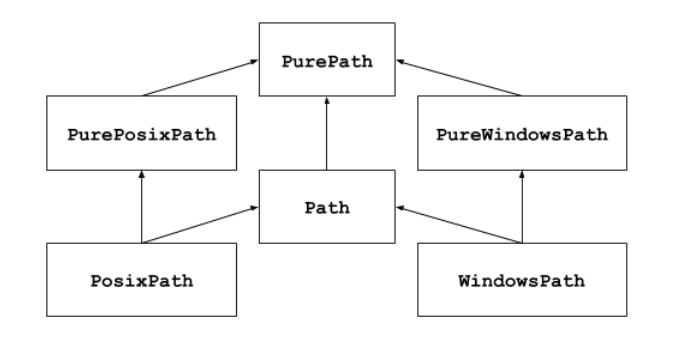
\includegraphics[scale=0.5]{IMG/Pathlib-01.png}
\caption{Hiérarchie des classes du module \texttt{pathlib}}
\end{center}
\end{figure}
\medskip

Le principe est le suivant: on crée un objet de type \textit{chemin} avec lequel nous disposons de diverses méthodes cohérentes et utiles nous permettant d'interagir avec cet objet. Le raisonnement clé du module est le fait de ne pas hériter de la classe \texttt{str} afin d'éviter tout potentiel incident lié à des opérations avec des chaînes de caractères représentant un chemin. Les objets \texttt{Path} sont des objets immuables. De par sa philosophie le module \texttt{pathlib} se place à l'opposée d'\texttt{os.path} et de ses multiples fonctions.
\medskip

Illustrons cela avec un exemple aisément compréhensible:
\begin{verbatim}
    >>> from pathlib import Path
    >>> p = Path("/Chemin/vers/fichier.py")  # Instanciation de l'objet
    >>> p. parent  # Récupération du répertoire parent
    PosixPath('/Chemin/vers')
    >>> p.suffix  # Récupération de l'extension
    '.py'
\end{verbatim}
\medskip

\section{La classe \texttt{Path}}
Héritière de la classe \texttt{PurePath}, c'est la classe que nous utilisons le plus fréquemment, et c'est d'ailleurs pour cela qu'elle porte le nom le plus court. La classe \texttt{Path} permet de créer un objet représentant un chemin qui pointe sur un fichier ou un répertoire\footnote{En fait, elle permet d'instancier un chemin concret de fichier ou de répertoire, présent ou non sur le système.}. Un tel objet est un objet de type \texttt{PosixPath} qui représente les chemins ds systèmes \textit{GNU/Linux} et \textit{MacOS}. Sur les systèmes \textit{Windows} sera créé un objet de type \texttt{WindowsPath}. A noter qu'il n'est pas possible d'instancier un objet \texttt{PosixPath} sur un objet \texttt{WindowsPath} et vice-et-versa.
\medskip

Il nous faut tout d'abord importer cette classe:
\begin{lstlisting}[caption=Import de la classe \texttt{Path}]
from pathlib import Path
\end{lstlisting}
\medskip

Illustrons par un exemple simple:
\begin{lstlisting}[caption=Un premier script à l'aide du module \texttt{pathlib}]
from pathlib import Path

user_dir = Path.home()  # Répertoire de l'utilisateur
current_dir = Path.cwd()  # Répertoire courant

# Création d'un objet :
way = Path("/Chemin/Vers/Fichier.py")
way_p = way.parent  # Retourne le répertoire parent

print(f"Répertoire de l'utilisateur : {user_dir}")
print(f"Répertoire courant : {current_dir}")
print(f"Répertoire parent de l'objet '{way}' : {way_p}")
\end{lstlisting}
\medskip

La sortie de ce script est alors la suivante:
\begin{verbatim}
    Répertoire de l'utilisateur : /home/krystof
    Répertoire courant : /home/krystof/Documents/DEVELOPPEMENT/Python/Module_
        pathlib/Presentation
    Répertoire parent de l'objet '/Chemin/Vers/Fichier.py' : /Chemin/Vers
\end{verbatim}
\medskip

\section{Concaténer des chemins}
Pour la concaténation nous n'avons pas à nous soucier, avec les objets récupérés, du sens des \textit{slashs} et \textit{antislashs} (Les barres obliques \texttt{/} et \texttt{\textbackslash}) puisque le système d'exploitation utilisé sera reconnu.
\medskip
\begin{verbatim}
    >>> from pathlib import Path
    >>> p = Path.home()
    >>> p / "New_dir"
    PosixPath('/home/krystof/New_dir')
    >>> p / "New_dir" / "fichier.py"  # Concaténation mutliple
    PosixPath('/home/krystof/New_dir/fichier.py')
\end{verbatim}
\medskip

Il est aussi possible d'user de la méthode \texttt{.joinpath()}:
\begin{verbatim}
    >>> p.joinpath("New_dir", "fichier.py")
    PosixPath('/home/krystof/New_dir/fichier.py')
    >>> p.joinpath("New_dir", "fichier.py").suffix
    '.py'
\end{verbatim}
\medskip

Avec la méthode \texttt{.joinpath()} et à l'aide du symbole de dépaquetage (\texttt{*}) nous pouvons réaliser une concaténation via une liste de noms:
\begin{verbatim}
    >>> p = Path.home()
    >>> reps_et_sous_reps = ['Projets', 'Bibpy', 'Files']
    >>> p.joinpath(*reps_et_sous_reps)
\end{verbatim}
\medskip

L'objet en sortie sera alors:
\begin{verbatim}
    PosixPath('/home/krystof/Projet/Bibpy/Files']
\end{verbatim}
\medskip

\section{Récupérer des informations sur un chemin}
Illustrons cela par un petit script:
\begin{lstlisting}[caption=Script avec recueils d'informations]
from pathlib import Path

p = Path.home()
chemin = p / "Dir" / "main.py"
chemin_complet = chemin.parent / chemin.name
print(f"Nom du fichier : {chemin.name}")
print(f"Nom du fichier (sans l'extension) : {chemin.stem}")
print(f"Extension du fichier : {chemin.suffix}")
print(f"Découpage du chemin : {chemin.parts}")
print(f"Vérification de l'existence su fichier : "
      f"{chemin.exists()}")
print(f"Le chemin pointe-t-il vers un répertroire ? "
      f"{chemin.is_dir()}")
print(f"Le chemin pointe-t-il vers un fichier ? "
      f"{chemin.is_file()}")
print(f"Répertoire parent: {chemin.parent}")
print(f"Chemin complet: {chemin_complet}")
\end{lstlisting}
\medskip

Ce qui nous donne en sortie:
\begin{verbatim}
    Nom du fichier : main.py
    Nom du fichier (sans l'extension) : main
    Extension du fichier : .py
    Découpage du chemin : ('/', 'home', 'krystof', 'Dir', 'main.py')
    Vérification de l'existence su fichier : False
    Le chemin pointe-t-il vers un répertroire ? False
    Le chemin pointe-t-il vers un fichier ? False
    Répertoire parent: /home/krystof/Dir
    Chemin complet: /home/krystof/Dir/main.py
\end{verbatim}
\medskip

Il existe la méthode \texttt{.suffixes} qui nous permet d'obtenir toutes les extensions d'un fichier, comme par exemple pour un fichier du type \texttt{archive.tar.gz}. Ce qui nous donnerait en sortie la liste suivante: \texttt{['.tar', '.gz']}.
\medskip

\section{Créer et supprimer des répertoires}
Nous allons tout d'abord créer un répertoire dans lequel nous pourrons réaliser divers tests, puis à la fin de cette sections nous supprimerons ce répertoire ainsi que tout son contenu. Créons ce répertoire sur notre \textit{Bureau} à l'aide du script suivant:
\begin{lstlisting}[caption=Créer un répertoire sur le bureau de l'utilisateur]
from pathlib import Path

test_rep = Path.home() / "Bureau" / "TestRep"
test_rep.mkdir()  # Méthode .mkdir() pour créer le répertoire
\end{lstlisting}
\medskip

Si le répertoire existe déjà, la méthode \texttt{.mkdir()} va lever une exception de type \texttt{FileExistsError} (relancer le script ci-dessus pour le vérifier). Pour palier à cette levée d'exception il est nécessaire d'utiliser le paramètre \texttt{exist\_ok} ayant pour valeur \texttt{True}:
\begin{lstlisting}[caption=Avec \texttt{exist\_ok=True}]
test_rep.mkdir(exist_ok=True)
\end{lstlisting}
\medskip

Il est possible de créer un répertoire contenant une arborescence de répertoires. Ajouter les lignes suivantes au script ci-dessus:
\begin{lstlisting}[caption=Créer une arborescence de répertoires]
test_rep = test_rep / "SousRep1" / "SousRep2" / "SousRep3"
test_rep.mkdir(exist_ok=True, parents=True)
print(test_rep)
\end{lstlisting}
\medskip

La ligne \texttt{print(test\_rep} vient afficher l'arborescence alors créée:
\begin{verbatim}
    /home/krystof/Bureau/TestRep/SousRep1/SousRep2/SousRep3
\end{verbatim}
\medskip

La création d'un fichier obéit au même principe mais avec la méthode \texttt{.touch()}. Ajouter les lignes suivantes au script:
\begin{lstlisting}[caption=Créer un fichier]
# Créer un fichier dans le répertoire 'SousRep3'
fichier = test_rep / "README.txt"
fichier.touch()
\end{lstlisting}
\medskip

Pour supprimer un fichier il nous faut utiliser la méthode \texttt{.unlink()}. Enfin, pour supprimer un répertoire nous disposons de la méthode \texttt{.rmdir()}. Cependant, si le répertoire contient des éléments, l'emploi de cette méthode va lever une exception de type \texttt{OSError}. Pour supprimer un répertoire avec l'ensemble de son contenu nous devons faire appel au module \texttt{shutil}. Ajoutons ces lignes à la fin de notre script, en s'assurant au préalable de l'import du module:
\begin{lstlisting}[caption=La méthode \texttt{.rmtree()} du module \texttt{shutil}]
import shutil

# ... code du script ...

# Suppression ou pas
o_n, supprime = ["o", "n"], ""
while supprime not in o_n:
    supprime = input("Voulez-vous supprimer le répertoire de "
                     "test créé précédemment (o/n) : ").lower()
    if supprime == "o":
        shutil.rmtree(Path.home() / "Bureau" / "TestRep")
\end{lstlisting}
\medskip

\section{Lire et écrire dans un fichier}
Avec le module \texttt{pathlib} il est possible d'écrire dans un fichier  et de lire son contenu sans en passer par un \textit{context manager} avec lequel nous ouvrons et fermons classiquement un fichier. Voyons cela par le script ci-dessous:
\begin{lstlisting}[caption=Ecriture dans un fichier de type \texttt{.txt}] 
from pathlib import Path


def oui_ou_non(question: str) -> bool:
    """L'utilisateur doit saisir 'o' ou 'n'."""
    o_n, reponse = ["o", "n"], ""
    while reponse not in o_n:
        reponse = input(f"{question}(o/n) ").lower()
        if reponse not in o_n:
            print("Veuillez répondre par 'o' ou 'n'...")
            return oui_ou_non(question)
        elif reponse == "n":
            return False
    return True


# Création du fichier test :
file_text = Path.home() / "Bureau" / "file_test.txt"
file_text.touch(exist_ok=True)

# Ecrire dans fichier
if oui_ou_non(f"Voulez-vous écrire dans le fichier "
              f"{file_text.name} ? "):
    # Méthode .write_text(texte_à_insérer) :
    file_text.write_text(input("Veuillez saisir le texte à "
                               "saisir : "))
if oui_ou_non(f"Voulez-vous supprimer le fichier "
              f"{file_text.name} ?"):
    file_text.unlink()  # Méthode de suppression d'un fichier
if file_text.exists():  # Si le fichier existe
    # Méthode de lecture du contenu du fichier.
    print(f"Texte du fichier : {file_text.read_text()}")
\end{lstlisting}
\medskip

\section{Scanner un répertoire}
Voyons comment récupérer tous les répertoires et fichiers, contenus dans un répertoire:
\begin{lstlisting}[caption=La méthode \texttt{.iterdir()}]
from pathlib import Path

for f in Path.home().iterdir():  # Répertoire de l'utilisateur
    print(f.name)
\end{lstlisting}
\medskip

L'emploi de la fonction \texttt{.iterdir()} retourne un objet de type \textit{générateur} (\textit{generator}) sur lequel il est possible d'itérer.
\medskip

Le script ci-dessus nous affiche l'ensemble des fichiers et répertoires, y compris ceux cachés (préfixés par un point), contenus dans le répertoire sur lequel la méthode \texttt{.iterdir()} est appliquée:
\begin{verbatim}
Téléchargements
.gitconfig
.cinnamon
Hasard.py
.cache
.vscode
.profile
.mozilla
.ipython
.var
.bashrc
.python_history
.virtualenvs
.java
.themes
.pyenv
Images
...etc
\end{verbatim}
\medskip

A l'aide de compréhensions de listes nous pouvons affiner les recherches:
\begin{lstlisting}[caption=La méthode \texttt{.iterdir()} avec des compréhensions de liste]
# Retourne la liste des répertoires :
print([f for f in Path.home().iterdir() if f.is_dir()])  
# Retourne la liste des fichiers :
print([f for f in Path.home().iterdir() if f.is_file()])  
\end{lstlisting}
\medskip

Effectuer une recherche selon les types de fichiers avec la méthode \texttt{.glob(motif)}, où \texttt{motif} représente le type de fichiers recherchés:
\begin{lstlisting}[caption=La méthode \texttt{.glob(motif)}]
# Affiche l'ensemble des fichiers de type .png :
for f in Path.Home().glob("*.png"):
    print(f.name)
\end{lstlisting}
\medskip

Il existe aussi la méthode \texttt{.rglob(motif)} qui permet la récursivité, et qui va donc effectuer la recherche dans l'ensemble des sous-répertoires.
\medskip

\section{Quelques exemples concrets de l'utilisation du module \texttt{pathlib}}
\subsection*{Modifier le nom d'un fichier}
\begin{verbatim}
    >>> from pathlib import Path
    >>> file_img = Path.home() / "Images" / "5452.jpg"
    >>> file_img.parent / (file_img.stem + "-Photo_id" + file_img.suffix)
    PosixPath('/home/krystof/Images/5452-Photo_id.jpg')
\end{verbatim}
\medskip

A partie de là nous pouvons imaginer un script qui permettrait de renommer en masse des fichiers...
\medskip

\subsection*{Trier des fichiers selon l'extension}
Le script qui suit permet de trier les fichiers présents dans le répertoire \texttt{Téléchargements} de l'utilisateur.
\begin{lstlisting}[caption=Trier des fichiers]
"""Tri des fichiers selon leur extension."""

from pathlib import Path  # Import de la classe 'Path'

dirs = {  # "Extensions": "Répertoire cible"
    ".png": "Images",
    ".jpeg": "Images",
    ".jpg": "Images",
    ".gif": "Images",
    ".pdf": "Documents_texte",
    ".docx": "Documents_texte",
    ".txt": "Documents_texte",
    ".odt": "Documents_texte",
    ".ods": "Documents_texte",
    ".deb": "Archives_Deb",
    ".zip": "Archives",
    ".gz": "Archives",
    ".xz": "Archives",
    ".tgz": "Archives",
    ".rpm": "Archives",
    ".gpx": "Divers",
    ".xlsx": "Divers",
    ".exe": "Divers",
    ".tex": "Divers",
    ".gpg": "Divers",
    ".ics": "Divers",
    ".eml": "Divers",
    ".py": "Fichiers_Python",
    ".iso": "Fichiers_ISO"
}

rep_a_trier = Path.home() / "Téléchargements"
# Récupérer l'ensemble des chemins qui correspondent uniquement 
# à des fichiers:
all_files = [f for f in rep_a_trier.iterdir() if f.is_file()]
# Boucle pour traiter chacun des fichiers de la liste:
for f in all_files:
    rep_de_redirection = rep_a_trier / dirs.get(f.suffix, 
                                            "Extentions_autres")
    rep_de_redirection.mkdir(exist_ok=True)
    # Déplacement du fichier :
    f.rename(rep_de_redirection / f.name)  
\end{lstlisting}
\medskip

\section{Les méthodes de la classe \texttt{Path}}
Pour connaître l'ensemble des méthodes applicables avec la classe \texttt{Path}:
\begin{verbatim}
    >>> dir(Path)
    ['__bytes__', '__class__', '__delattr__', '__dir__', '__doc__', 
    '__enter__', '__eq__', '__exit__', '__format__', '__fspath__', '__ge__', 
    '__getattribute__', '__getstate__', '__gt__', '__hash__', '__init__', 
    '__init_subclass__', '__le__', '__lt__', '__module__', '__ne__', 
    '__new__', '__reduce__', '__reduce_ex__', '__repr__', '__rtruediv__', 
    '__setattr__', '__sizeof__', '__slots__', '__str__', '__subclasshook__', 
    '__truediv__', '_cached_cparts', '_cparts', '_drv', 
    '_format_parsed_parts', '_from_parsed_parts', '_from_parts', '_hash', 
    '_make_child', '_make_child_relpath', '_parse_args', '_parts', '_pparts', 
    '_root', '_scandir', '_str', 'absolute', 'anchor', 'as_posix', 'as_uri', 
    'chmod', 'cwd', 'drive', 'exists', 'expanduser', 'glob', 'group', 
    'hardlink_to', 'home', 'is_absolute', 'is_block_device', 
    'is_char_device', 'is_dir', 'is_fifo', 'is_file', 'is_mount', 
    'is_relative_to', 'is_reserved', 'is_socket', 'is_symlink', 'iterdir', 
    'joinpath', 'lchmod', 'link_to', 'lstat', 'match', 'mkdir', 'name', 
    'open', 'owner', 'parent', 'parents', 'parts', 'read_bytes', 
    'read_text', 'readlink', 'relative_to', 'rename', 'replace', 'resolve', 
    'rglob', 'rmdir', 'root', 'samefile', 'stat', 'stem', 'suffix', 
    'suffixes', 'symlink_to', 'touch', 'unlink', 'with_name', 'with_stem', 
    'with_suffix', 'write_bytes', 'write_text']
\end{verbatim}
\medskip

Pour un descriptif de certaines de ces méthodes, voir les tableaux des pages \pageref{pathlib_1} et \pageref{pathlib_2}. \medskip

Pour un tableau des correspondances avec les outils du module \texttt{os} on se reportera à l'adresse suivante: \\ \url{https://docs.python.org/fr/3/library/pathlib.html\#correspondance-to-tools-in-} \\
\url{the-os-module}
\medskip

\begin{table}[h]\label{pathlib_1}
\begin{center}
\begin{tabular}{|p{4cm}|p{10.5cm}|}
\hline
\textbf{Méthode} & \textbf{Action} \\
\hline
\texttt{Path.chmod(mode, *, follow\_symlinks=True)} & Change les permissions du fichier à l'instar de \texttt{os.chmod}. Exemple: \texttt{fichier.chmod(0o777)} \\
\hline
\texttt{Path.cwd()} & Retourne un nouveau chemin représentant le dossier courant, tel que renvoyé par \texttt{os.getcwd()}. \\
\hline
\texttt{Path.exists()} & Permet de vérifier si le chemin existe. Retourne \texttt{True} ou \texttt{False}. \\
\hline
\texttt{Path.expanduser()} & Un \texttt{PosixPath('\~{}/Documents')} auquel on applique la méthode \texttt{expanduser()} retournera l'objet suivant: \texttt{PosixPath('/home/krystof/ Documents')} \\
\hline
\texttt{Path.glob(motif)} & Permet une itération dans les répertoires afin de lister les fichiers correspondant au motif. Ainsi l'instruction \texttt{list(chemin.glob('**/*.py))} va lister l'ensemble des fichiers \texttt{.py} présent dans le répertoire ciblé. \\
\hline
\texttt{Path.home()} & Retourne un nouveau chemin représentant le répertoire racine de l'utilisateur, tel que renvoyé par \texttt{os.path.expanduser('\~{}')}. \texttt{PosixPath('/home/krystof')} sera affiché en sortie, tandis qu'avec \texttt{os.path.expanduser('\~{}')} nous obtiendrons \texttt{'/home/krystof'}. \\
\hline
\texttt{Path.is\_dir()} & Vérifie si le chemin est celui d'un répertoire. Retourne une valeur booléenne. \\
\hline
\texttt{Path.is\_file()} & Vérifie si le chemin est celui d'un fichier. Retourne une valeur booléenne. \\
\hline
\texttt{Path.iterdir()} & Permet d'itérer sur l'ensemble des fichiers du répertoire (avec une boucle \texttt{for} pour une utilisation classique). Exemple de la compréhension de liste \texttt{[x for x in chemin.iterdir() if x.is\_dir()]} qui permet de lister les répertoires du répertoire cible. \\
\hline
\texttt{Path.mkdir(mode=0o777 , parents=False, exist\_OK=False)} & Pour créer un répertoire. \\
\hline
\texttt{Path.open(mode='r', buffering=-1, encoding=None, errors=None, newline=None)} & Permet d'ouvrir un fichier à l'instar de la fonction native \texttt{open()}. Utilisations: \texttt{chemin\_fichier.open()} ou \texttt{with chemin\_fichier.open() as f:}. \\
\hline
\texttt{Path.rmdir()} & Supprime le répertoire donné. Celu-ci doit être vide. \\
\hline
\texttt{Path.samefile(autre\_ path)} & Retourne \texttt{True} ou \texttt{False} si le chemin pointe vers le même fichier que \texttt{autre\_path}, qui peut être un chemin ou une chaîne de caractères. La sémantique est similaie à \texttt{os.path.samefile()} et \texttt{os.path.samestat()}. \\
\hline
\texttt{Path.stat(*, follow\_symlinks=True)} & Retourne un objet contenant des informations sur le chemin. \\
\hline
\texttt{Path.touch(mode=0o666
, exist\_ok=True)} & Créer un fichier, s'il n'existe pas, avec le mode d'accès donné. \\
\hline
\texttt{Path.unlink(missing\_
ok=False)} & Supprime le fichier (ou lien symbolique). Utiliser \texttt{Path.rmdir()} si le chemin pointe vers un répertoire. Si \texttt{missing\_ok} est à \texttt{True} (\texttt{False} étant la valeur par défaut) l'exception \texttt{FileNotFoundError} est ignorée (même comportement que la commande \textit{posix} \texttt{rm -f}. \\
\hline
\end{tabular}
\caption{Les méthodes de la classe \texttt{Path} (1).}
\end{center}
\end{table}
\medskip

\begin{table}[h]\label{pathlib_2}
\begin{center}
\begin{tabular}{|p{4cm}|p{10.5cm}|}
\hline
\textbf{Méthode} & \textbf{Action} \\
\hline
\texttt{Path.write\_text(
donnée, encoding=None, errors=None, newline=None)} & Ouvre le fichier pointé en mode texte, y inscrit \texttt{donnée} puis ferme le fichier. S'il existe, le fichier du même nom est écrasé. Les paramètres optionnels ont la même signification que la fonction native \texttt{open()}. \\
\hline
\texttt{Path.owner()} & \texttt{chemin.owner()} donne en sortie \texttt{'krystof'}. \\
\hline
\texttt{Path.rename(cible)} & Renomme le chemin avec le nom 'cible'. \\
\hline
\texttt{Path.replace(cible)} & Comme \texttt{Path.rename(cible)}, mais écrase le chemin renommé s'il existe. \\
\hline
\texttt{Path.resolve(strict=
False)} & Retourne le chemin absolu en résolvant tous les liens symboliques afin de normaliser ce chemin. \\
\hline
\texttt{Path.rglob(motif)} & Similaire à la méthode \texttt{Path.glob()}. Retourne de façon récursive (en explorant les sous-répertoires) tous les fichiers correspondant au motif donné. \\
\hline
\texttt{Path.symlink\_to(cible
, target\_is\_directory=
False} & Faire de ce chemin un lien symbolique qui point vers \texttt{cible}. \\
\hline
\texttt{Path.write\_bytes(don
née)} & Ouvre le fichier pointé en mode binaire, y écrit \texttt{donnée} puis ferme le fichier. S'il existe, le fichier du même nom est écrasé. \\
\hline
\end{tabular}
\caption{Les méthodes de classe la  \texttt{Path} (2).}
\end{center}
\end{table}
\medskip

\section{Sources pour la rédaction de ce chapitre}
\begin{itemize}
	\item[-] \textit{Gérer des chemins de fichiers avec \texttt{pathlib}}, par Thibault \textsc{Houdon} - \url{https://www.docstring.fr/blog/gere-des-chemins-de-fichiers-avec-pathlib}
	\item[-] \textit{\texttt{pathlib} - Chemins de système de fichiers orientés objet} - \url{https://docs.python.org/fr/3/library/pathlib.html}
	\item[-] \textit{PEP 428 – The \texttt{pathlib} module – object-oriented filesystem paths} (trad. \textit{PEP 428 - Le module \texttt{pathlib} - Chemins d'accès au système de fichiers orientés objet}), par Antoine \textsc{Pitrou}, 30 juillet 2012 - \url{https://peps.python.org/pep-0428/}  
\end{itemize}
\medskip

\subsection*{Documentation complémentaire}
\begin{itemize}
	\item[-] \textit{Python 3's \texttt{pathlib} Module: Taming the File System} (trad. \textit{Le module \texttt{pathlib} de Python 3 : Apprivoiser le système de fichiers}), par Geir Arne \textsc{Hjelle}, 23 avril 2018 - \url{https://realpython.com/python-pathlib/}
	\item[-] \textit{Working With Files in Python} (trad. \textit{Travailler avec des fichiers en Python}), par Vuyisile \textsc{Ndlovu}, 21 janvier 2019 - \\ \url{https://realpython.com/working-with-files-in-python/}
	\item[-] \textit{How to Get a List of All Files in a Directory With Python} (trad. \textit{Comment obtenir la liste de tous les fichiers d'un répertoire avec Python ?}), par Ian \textsc{Currie}, 28 novembre 2022 - \url{https://realpython.com/get-all-files-in-directory-python/}
\end{itemize}


\part{\textcolor{cyan}{\textit{Python} en profondeur}}

%%%%%%%%%%%%
%%% Chapitre 1 %%%
%%%%%%%%%%%%
\chapter{Ecrire du code \texttt{Python} selon le \texttt{PEP8}}
\texttt{PEP} signifie \textit{Python Enhancement Proposal} (\textit{Proposition d'amélioration de Python}), et il en existe plusieurs. Un \texttt{PEP} est un document qui décrit les nouvelles fonctionnalités proposées pour \texttt{Python} et en documente les aspects. Le \texttt{PEP8}\footnote{\textit{Style Guide for Python Code} - \url{https://peps.python.org/pep-0008/}} fournit des directives et des bonnes pratiques sur la façon d'écrire du code \texttt{Python}. Il a été rédigé en 2001 par Guido \textsc{van Rossum}, Barry \textsc{Warsaw} et Nick \textsc{Coghlan}. L'objectif principal du \texttt{PEP8} est d'améliorer la lisibilité et la cohérence du code Python.
\medskip

En tant que débutant, suivre les règles de la \texttt{PEP 8} peut rendre l'apprentissage de \texttt{Python} beaucoup plus agréable. Suivre le \texttt{PEP 8} est particulièrement important si vous cherchez un emploi dans le domaine du développement. Écrire un code clair et lisible est une preuve de professionnalisme. Cela indique à un employeur que vous savez comment bien structurer votre code. Si vous avez plus d'expérience dans l'écriture de code \texttt{Python}, vous devrez peut-être collaborer avec d'autres personnes. L'écriture d'un code lisible est ici cruciale. 

\section{Les conventions de nommage}
Dans le codage il est nécessaire de définir des variables, des fonctions, des classes, bref des objets qu'il nous faudra nommer. Le choix de ces noms devra rendre explicite le contenu de l'objet. Ainsi, si une valeur doit représenter un âge, autant nommer la variable \texttt{age} plutôt que \texttt{a}, ce qui rendra votre code plus lisible et facilitera son débogage.

\subsection*{Les styles de nommage selon l'objet :}
\begin{table}{!h}
\begin{center}
\begin{tabular}{|p{2cm}|p{7cm}|p{3cm}|}
\hline
\textbf{Type} & \textbf{Convention de nommage} & \textbf{Exemples} \\
\hline
Fonction & Nom en minuscules, et si plusieurs mots utilisés, ils sont séparés par un underscore. & \texttt{fonction}, \texttt{ma\_fonction} \\
\hline
Variable & Comme pour les fonctions. Possibilité de n'utiliser qu'une seule lettre. & \texttt{x}, \texttt{variable}, \texttt{ma\_variable} \\
\hline
Classe & Chaque mot du nom débute par une majuscule, et ils ne sont pas séparés. C'est le style \textit{camel case}. & \texttt{NomDeClasse} \\
\hline
Méthodes (de classe) & Comme pour les fonctions. & \texttt{methode\_de\_classe} \\
\hline
Constante & Nom en majuscules, et si plusieurs mots utilisés, ils sont séparés par un underscore. & \texttt{X}, \texttt{CONST}, \texttt{MA\_CONSTANTE} \\
\hline
Module  et package & Comme pour les fonctions. & \texttt{module.py}, \texttt{mon\_module.py}, \texttt{nom\_package.py} \\
\hline
\end{tabular}
\caption{Les styles de nommage en \texttt{Python}.}
\end{center}
\end{table}
\medskip

\subsection*{Le choix des noms:}
Il est pertinent de choisir des noms descriptifs pour nommer ses objets, qui décrivent clairement l'objet. Cela participe d'ailleurs à rendre le code plus lisible, notamment cela aide le développeur quand il reprend son code plusieurs jours ou plusieurs semaines après. Par exemple choisir comme nom de variable les termes \texttt{nom} ou \texttt{name} pour stocker le nom d'une personne, ou bien comme nom de fonction \texttt{multiplie\_par\_deux} ou \texttt{multiply\_by\_two}.
\medskip

\section{Présentation du code}
\subsection*{Les lignes vides:}
Les lignes vides, peuvent améliorer considérablement la lisibilité de votre code. Un code peu aéré peut être écrasant et difficile à lire, de même, trop de lignes vides lui donne un aspect très clairsemé. Voici quelques règles pour améliorer la lisibilité de vote code:
\begin{itemize}
	\item Deux lignes vides séparent les fonctions et les classes de haut niveau.
	\item Une seule ligne sépare les méthodes d'une classe.
	\item Il est possible d'utiliser une ligne de séparation entre diverses étapes d'une fonction, si cette fonction dispose d'un code relativement long.
\end{itemize}
\medskip

Si les lignes vides sont utilisées avec soin, elles peuvent améliorer considérablement la lisibilité de votre code. Cela aide le lecteur à comprendre visuellement comment est structuré le code. 
\medskip

\subsection*{Longueur maximale des lignes et saut de ligne}
Le \texttt{PEP 8} suggère que les lignes soient limitées à 79 caractères,  ce qui permet d'avoir plusieurs fichiers ouverts l'un à côté de l'autre. Bien sûr, il n'est pas toujours possible de limiter les déclarations à 79 caractères, et le \texttt{PEP 8} propose des moyens de permettre aux instructions de s'étendre sur plusieurs lignes.
\medskip

Voici quelques exemples recommandés par le \texttt{PEP 8}:
\begin{description}
	\item[Avec des parenthèses]: 
	\begin{lstlisting}
	def fonction(arg_un, arg_deux,
                 arg_trois, arg_quatre):
        return arg_un
	\end{lstlisting}
	\item[utilisation des \textit{antislashes} pour couper les lignes]:
	\begin{lstlisting}
	from mon_package import meth1, \
        meth2, meth3
	\end{lstlisting}
	\item[Saut de ligne avant les opérateurs]:
	\begin{lstlisting}
	total = (valeur_un
             + valeur_deux
             - valeur_trois)
	\end{lstlisting}
\end{description}
\medskip

\section{Indentation}
L'indentation est extrêmement importante en \texttt{Python}. Le niveau d'indentation des lignes de code en \texttt{Python }détermine la manière dont les instructions sont regroupées. Les principales règles d'indentation énoncées par la \texttt{PEP 8} sont les suivantes :
\begin{itemize}
	\item Utiliser 4 espaces consécutifs pour indiquer l'indentation.
	\item Préférer les espaces aux tabulations.
\end{itemize}
\medskip

Lorsque vous utilisez des sauts de ligne pour limiter les lignes à moins de 79 caractères, il est utile d'utiliser l'indentation pour améliorer la lisibilité. Elle permet au lecteur de faire la distinction entre deux lignes de code et une seule ligne de code qui s'étend sur deux lignes. Il existe deux styles d'indentation que vous pouvez utiliser.
\begin{itemize}
    \item Le premier consiste à aligner le bloc indenté avec le délimiteur d'ouverture :
    \begin{lstlisting}
    def fonction(arg_un, arg_deux,
                 arg_trois, arg_quatre):
        return arg_un
	\end{lstlisting}
	\item Un autre style d'indentation est l'indentation suspendue. Il s'agit d'un terme typographique qui signifie que toutes les lignes d'un paragraphe ou d'une déclaration, sauf la première, sont mises en retrait:
	\begin{lstlisting}
	var = fonction(
        arg_un, arg_deux,
        arg_trois, arg_quatre)
	\end{lstlisting}
\end{itemize}
\medskip

Il arrive parfois que 4 espaces seulement soient nécessaires pour s'aligner sur le délimiteur d'ouverture. Cela se produit souvent dans les instructions \texttt{if} qui s'étendent sur plusieurs lignes, car le \texttt{if}, l'espace et la parenthèse ouvrante représentent 4 caractères. Dans ce cas, \texttt{PEP 8} fournit deux alternatives pour aider à améliorer la lisibilité :
\begin{itemize}
	\item Ajouter un commentaire après la condition finale.
	\begin{lstlisting}
	x = 5
    if (x > 3 and
        x < 10):
        # Les deux conditions sont remplies
        print(x)
	\end{lstlisting}
	\item Ajouter une indentation supplémentaire sur la suite de la ligne.
	\begin{lstlisting}
	x = 5
    if (x > 3 and
            x < 10):
        print(x)
	\end{lstlisting}
\end{itemize}
\medskip

Avec les fonctions, il est préférable d'utiliser une double indentation sur la suite de la ligne. Cela permet de faire la distinction entre les arguments de fonction et le corps de la fonction, ce qui améliore la lisibilité :
\begin{lstlisting}
def fonction(
        arg_un, arg_deux,
        arg_trois, arg_quatre):
    return arg_un
\end{lstlisting}
\medskip

Les continuations de ligne permettent de rompre les lignes à l'intérieur des parenthèses, des crochets ou des accolades. Il est facile d'oublier l'accolade fermante, mais il est important de la placer à un endroit judicieux. Sinon, cela peut perturber le lecteur. Le \texttt{PEP 8} fournit deux options pour la position de l'accolade fermante dans le cadre des continuations de ligne implicites :
\begin{itemize}
	\item Alignez l'accolade fermante avec le premier caractère de la ligne précédente.
	\begin{lstlisting}
	liste_de_nombres = [
        1, 2, 3,
        4, 5, 6,
        7, 8, 9
        ]
	\end{lstlisting}
	\item Alignez l'accolade fermante avec le premier caractère de la ligne qui commence la construction.
	\begin{lstlisting}
	liste_de_nombres = [
        1, 2, 3,
        4, 5, 6,
        7, 8, 9
    ]
	\end{lstlisting}
\end{itemize}
\medskip

\section{Les commentaires}
Un commentaire doit permettre de comprendre facilement le code auquel le commentaire s'applique. Voici quelques points essentiels à retenir lorsque vous ajoutez des commentaires à votre code :
\begin{itemize}
	\item Limitez la longueur de ligne des commentaires et des \textit{docstrings} à 72 caractères.
    \item Utilisez des phrases complètes, commençant par une majuscule.
    \item Veillez à mettre à jour les commentaires si vous modifiez votre code.
\end{itemize}
\medskip

\subsection*{Les blocs de commentaires}
Utilisez les commentaires de bloc pour documenter une petite section de code. Ils sont importants car ils aident les autres à comprendre l'objectif et la fonctionnalité d'un bloc de code donné. \texttt{PEP 8} fournit les règles suivantes pour la rédaction des commentaires de bloc :
\begin{itemize}
	\item Indenter les blocs de commentaires au même niveau que le code qu'ils décrivent.
    \item Commencez chaque ligne par un \texttt{\#} suivi d'un simple espace.
    \item Séparer les paragraphes par une ligne contenant un seul \texttt{\#}.
\end{itemize}
\medskip

Parfois, si le code est très technique, il est nécessaire d'utiliser plus d'un paragraphe dans un commentaire de bloc.
\begin{lstlisting}
# Voici un premier paragraphe
# pour mon commentaire de bloc
#
# Et après un saut de ligne (avec #)
# je m'attaque au second paragraphe
\end{lstlisting}
\medskip

\subsection*{Commentaires de ligne unique de code}
Ils sont destinés à expliciter le code d'une seule ligne. Le \texttt{PEP 8} propose les règles suivantes:
\begin{itemize}
	\item Ils doivent être utilisés avec parcimonie.
	\item Ils doivent être écrits sur la même ligne que le code auquel ils font références.
	\item Les séparer par deux espaces ou plus du code.
	\item Ils débutent par \texttt{\#} suivi d'un espace unique.
	\item Ils ne s'utilisent pas pour expliquer ce qui est aisément compréhensible. 
\end{itemize} 
\medskip

Les commentaires de ligne unique de code peuvent rapidement encombrer votre code, les commentaires de bloc sont alors à privilégier.
\medskip

\subsection*{Les \textit{docstrings}}
Les \textit{docstrings}, sont des chaînes entre guillemets doubles (\texttt{"""}) ou simples (\texttt{'''}) qui apparaissent sur la première ligne de toute fonction, classe, méthode ou module. Le \texttt{PEP 257}\footnote{\url{https://peps.python.org/pep-0257/} - Voir aussi un guide assez complet sur la documentation du code à l'adresse suivante : \url{https://realpython.com/documenting-python-code/} - Voir aussi le chapitre \textit{Documenter son code et son projet} page \pageref{documentercodeprojet}.} leur est consacré.
\medskip

\section{Espaces blancs dans les expressions et les déclarations}
Les espaces blancs peuvent être très utiles dans les expressions et les déclarations lorsqu'ils sont utilisés correctement. S'il n'y a pas assez d'espace blanc, le code peut être difficile à lire, car tout est regroupé. S'il y a trop d'espaces blancs, il peut être difficile de combiner visuellement des termes connexes dans une déclaration.
\medskip

\subsection*{Espaces blancs autour des opérateurs binaires
}
Les opérateurs d'affectation (\texttt{=}, \texttt{+=}, \texttt{-=}, etc.), de comparaison (\texttt{==}, \texttt{!=}, \texttt{>}, \texttt{<}. \texttt{>=}, \texttt{<=}, \texttt{is}, \texttt{is not}, \texttt{in}, \texttt{not in}) et booléens (\texttt{and}, \texttt{not}, \texttt{or}) doivent être entourés d'un simple espace de chaque côté.
\medskip

Cepedanr lorsque le signe \texttt{=} est utilisé pour attribuer une valeur par défaut à un argument de fonction, ne l'entourez pas d'espaces.
\medskip

Lorsqu'il y a plus d'un opérateur dans une instruction, l'ajout d'un espace unique avant et après chaque opérateur peut prêter à confusion. Il est préférable de n'ajouter des espaces qu'autour des opérateurs ayant la priorité la plus faible, en particulier lors de manipulations mathématiques : 
\begin{lstlisting}
y = x**2 + 5
z = (x+y) * (x-y)
\end{lstlisting}
\medskip

Cela s'applique aussi avec les instructions comme \texttt{if} :
\begin{lstlisting}
if x>5 and x%2==0:
    print('x est plus grand que 5 et est un nombre pair')
\end{lstlisting}

Vous êtes bien entendu libre de choisir ce qui est le plus clair.
\medskip

Les mêmes règles s'appliquent aux \textit{slices} : 
\begin{lstlisting}
liste1[x+1 : x+2]
liste2[x+1 : x+2 : x+3]
liste3[x+1 : x+2 :]
\end{lstlisting}
\medskip

\subsection*{Quand éviter d'ajouter des espaces blancs}
Dans certains cas, l'ajout d'espaces blancs peut rendre le code plus difficile à lire. Trop d'espaces blancs peuvent rendre le code trop clairsemé et difficile à suivre. La \texttt{PEP 8} donne des exemples très clairs de cas où les espaces blancs sont inappropriés. L'endroit le plus important pour éviter d'ajouter des espaces blancs est la fin d'une ligne. C'est ce qu'on appelle les espaces blancs de fin de ligne. Il est invisible et peut produire des erreurs difficiles à repérer.
\medskip

Quelques exemples de recommandation :
\begin{lstlisting}
ma_liste = [1, 2, 3]
print(x, y)  # x et y étant des variables
ma_fonction(3)  # Appel de fonction
ma_liste[3]
mon_tuple = (1,)
var1 = 5
var2 = 6
un_long_nom_de_variable = 7
\end{lstlisting}
\medskip

Il existe d'autres cas où la \texttt{PEP 8} déconseille l'ajout d'espaces supplémentaires, notamment à l'intérieur des parenthèses, ainsi qu'avant les virgules et les deux-points.
\medskip

\section{Recommandations en matière de programmation
}
Le \textit{Zen de \texttt{Python}} dit : \og \textit{Le simple est préférable au complexe}\fg{}.
\medskip

Voici les principales recommandations:
\medskip

\begin{itemize}
	\item Ne  pas comparer pas les valeurs booléennes  (\texttt{True} ou \texttt{False} en utilisant un opérateur d'équivalence:
	\begin{lstlisting}
	if mon_booleen:
	\end{lstlisting}
	\item Utiliser le fait que les séquences vides sont fausses quand elles sont évaluer avec l'instruction \texttt{if}:
	\begin{lstlisting}
	ma_liste = []
	if not ma_liste:
	    print("La liste est vide")
	\end{lstlisting}
	\item Utiliser \texttt{is not} plutôt que \texttt{not ... is} dans les instructions \texttt{if}:
	\begin{lstlisting}
	if not x is None:
	    return 'x existe !'
	\end{lstlisting}
    \item Ne pas utiliser \texttt{if x :} lorsque l'on souhaite déclarer \texttt{if x is not None :} car parfois on peut avoir une fonction avec des arguments qui sont \texttt{None} par défaut, ce qui peut être source d'erreur.
    \begin{lstlisting}
    if arg is not None:
        # Faire quelque chose avec arg...
    \end{lstlisting}
    \item Utiliser \texttt{.startswith()} et \texttt{.endswith()} au lieu du découpage en tranches:
    \begin{lstlisting}
    if nom_fichier.endswith('jpg'):
        print("Le fichier est un fichier image de type JPEG")
    \end{lstlisting}
\end{itemize}
\medskip

\section{Un code conforme à la \texttt{PEP 8}}
Si vous suivez la \texttt{PEP 8} à la lettre, vous pouvez garantir que vous aurez un code propre, professionnel et lisible. Vous en tirerez profit, ainsi que les développeurs avec qui vous collaborer sur un projet commun.
\medskip

Pour aider le développeur à rendre son code conforme à la \texttt{PEP 8}, il existe deux catégories d'outils: les \textit{linters} et les outils de formatage automatique.
\medskip

\subsection*{Les \textit{linters}}
Les \textit{linters} sont des programmes qui analysent le code et signalent les erreurs. Ils fournissent des suggestions sur la manière de corriger l'erreur. Les \textit{linters} sont particulièrement utiles lorsqu'ils sont installés comme extensions de votre éditeur de texte, car ils signalent les erreurs et les problèmes stylistiques pendant que vous écrivez.
\medskip

\begin{description}
	\item[\texttt{pycodestyle}] est un outil permettant de vérifier votre code \textit{Python} par rapport à certaines des conventions de style du \texttt{PEP 8}\footnote{\url{https://pypi.org/project/pycodestyle/}}.
	\begin{verbatim}
	    $ pip install pycodestyle  # Installation
	    $ pycodestyle mon_code.py  # Exécution
	    mon_code.py:1:17: E231 missing whitespace after ','
	    mon_code.py:2:21: E231 missing whitespace after ','
	    mon_code.py:6:19: E711 comparison to None should be 'if cond is None:'
	\end{verbatim}
	\item[\texttt{flake8}] est un outil qui combine un débogueur (\texttt{ pyflakes}) avec \texttt{pycodestyle} qui, via la ligne de commandes, va analyser le code et en indiquer les erreurs de formatage\footnote{\url{https://pypi.org/project/flake8/}}.
	\begin{verbatim}
	    $ pip install flake8
	    $ flake8 mon_code.py
	    mon_code.py:1:17: E231 missing whitespace after ','
	    mon_code.py:2:21: E231 missing whitespace after ','
	    mon_code.py:3:17: E999 SyntaxError: invalid syntax
	    mon_code.py:6:19: E711 comparison to None should be 'if cond is None:'
	\end{verbatim}
\end{description}
\medskip

\subsection*{Les outils de formatage automatique}
On retrouve ce type d'outils sous forme de programmes qui refactorisent automatiquement votre code pour le rendre conforme à la \texttt{PEP 8}, comme par exemple le programme \textit{black}. Sur la page du projet\footnote{\url{https://pypi.org/project/black/}} il est dit que \textit{black} \og \textit{rend la révison du code plus rapide}\fg{}.
\medskip

Installation de \textit{black} de façon globale sur le système:
\begin{verbatim}
    $ pip install black
\end{verbatim}
\medskip

Utilisation (s'utilise en ligne de commandes):
\begin{verbatim}
    $ black mon_code.py
    reformatted mon_code.py
    All done!
\end{verbatim}
\medskip


Par défaut \textit{black} limite la longueur des lignes à 88 caractères, au lieu de 79, mais nous pouvons modifier un tel comportement avec l'option \verb|--line-length flag|:
\begin{verbatim}
    $ black --line-length=79 mon_code.py
    reformatted mon_code.py
    All done!
\end{verbatim}
\medskip

Deux autres outils réalisent des formatages automatiques, similaires à ceux réalisés par \textit{black}: \textit{autopep8}\footnote{\url{https://pypi.org/project/autopep8/}} et \textit{yapf}\footnote{\url{https://pypi.org/project/yapf/}}. Et bien entendu à l'aide de \texttt{Pycharm}:
\begin{verbatim}
    Code > Reformat Code
\end{verbatim}

D'autre encore proposent des fonctionnalités plus spécialisées:
\begin{description}
	\item[\texttt{docformatter}]\footnote{Voir la \texttt{PEP 257}: \url{https://peps.python.org/pep-0257/}} pour formater les \textit{docstrings}. A installer avec \texttt{pip install}.
	\begin{verbatim}
	    $docformatter --in-place fichier.py
	\end{verbatim}
	\item[isort]: Organise les imports comme il se doit.  installer avec \texttt{pip install}.
	\begin{verbatim}
	    $isort fichier.py
	\end{verbatim}
\end{description}
\medskip

\chapter{Qualité du code \textit{Python} : Outils et bonnes pratiques}
\section{Qu’est-ce qu’un code de qualité ?}
Un code de qualité, selon ce qui fait consensus dans la communauté des développeurs, répond à trois principes cruciaux:
\begin{itemize}
	\item[-] Un code doit faire ce qu’il est censé faire.
	\item[-] C'est un code qui ne contient pas de défaut ou problème.
	\item[-] Il doit demeurer facile à lire, à maintenir et à étendre.
\end{itemize}
\medskip

Ne pas respecter ces trois dimensions expose à ce que le code:
\begin{description}
	\item[- ne fasse pas ce qu'il est censé faire :] Le respect des exigences est à la base de tout produit, logiciel ou autre. Nous créons des logiciels pour faire quelque chose. Si, au bout du compte, il ne le fait pas, alors il ne s'agit certainement pas d'un produit de qualité.
	\item[- présente des défauts et des problèmes :] Si les défauts provoquent des comportements indésirables, là aussi nous n'avons pas un produit de qualité.
	\item[- soit difficile à lire, à maintenir ou à étendre :] Si le code est complexe et alambiqué, il sera difficile pour une autre personne (voire vous-même) de le comprendre pour en corriger les éventuels défauts.
Il est également souhaitable qu'il soit facile d'ajouter de nouvelles fonctionnalités sans perturber les fonctionnalités précédentes. Si le code n'est pas facile à étendre, votre nouvelle fonctionnalité risque de perturber d'autres éléments.
\end{description}
\medskip

Pour améliorer la qualité d'un code il est souhaitable d'apporter une grande attention au style. Un guide de style a pour but de définir une manière cohérente d'écrire votre code. En règle générale, il s'agit d'une démarche cosmétique, qui ne modifie pas le résultat logique du code. Toutefois, certains choix stylistiques permettent d'éviter des erreurs logiques courantes.
En ce qui concerne \textit{Python}, il existe une norme bien acceptée. Elle a été rédigée, en partie, par l'auteur du langage de programmation Python lui-même. Le \texttt{PEP 8} fournit des conventions de codage pour le code \textit{Python}. Il est assez courant que le code \textit{Python} suive ce guide de style. C'est un bon point de départ car il est déjà bien défini (voir chapitre précédent).
\medskip

Il existe aussi le \texttt{PEP 257}, qui décrit les conventions pour les \textit{docstrings} de \textit{Python}, qui sont des chaînes destinées à documenter les modules, les classes, les fonctions et les méthodes. En prime, il existe des outils capables de générer de la documentation directement à partir du code (voir prochain chapitre).
\medskip

\section{Les \textit{linters}: des outils puissants pour améliorer son code}
Les petites erreurs, les incohérences stylistiques et les logiques dangereuses ne rendent pas un code agréable à regarder et à modifier. Les \textit{linters} permettent d'identifier ces problèmes. Il faut savoir que la plupart des éditeurs et des IDE ont la possibilité d'exécuter des \textit{linters} en arrière-plan, et ce  pendant que vous saisissez votre code. Les \textit{linters} analysent alors le code pour détecter différentes catégories de problèmes :
\begin{description}
	\item[- d'un point de vue logique :] erreurs de code, code dont les résultats sont potentiellement inattendus, modèles de code dangereux.
	\item[- d'un point de vue stylistique :] code non conforme aux conventions définies.
\end{description}
\medskip

Il existe également des outils d'analyse de code qui permettent d’en améliorer la qualité:
\begin{description}
	\item[\texttt{Flake8} :] Capable de détecter à la fois les défauts logiques et stylistiques. Il ajoute les vérifications de style et de complexité de \texttt{pycodestyle} à la détection logique de \texttt{PyFlakes}. Il combine les \textit{linters} suivants : \texttt{PyFlakes}, \texttt{pycodestyle} (\texttt{PEP 8}) et \texttt{Mccabe}.
	\item[\texttt{Pylama} :] C'est un outil d'audit de code composé d'un grand nombre de \textit{linters} et d'autres outils d'analyse de code. Il combine les éléments suivants : \texttt{pycodestyle}, \texttt{pydocstyle} (\texttt{PEP 257}), \texttt{PyFlakes}, \texttt{Mccabe}, \texttt{Pylint}, \texttt{Radon}, \texttt{gjslint}.
\end{description}
\medskip

Voici un tableau qui présente les divers \textit{linters} utilisables avec \textit{Python} :
\begin{table}[h]
\begin{center}
\begin{tabular}{|p{2.2cm}|p{1.8cm}|p{4.2cm}|p{5cm}|}
\hline
\textbf{\textit{linter}} & \textbf{Catégorie} & \textbf{Description} & \textbf{Sites Internet} \\
\hline 
\texttt{Pylint} & Logique et style & Vérifie les erreurs, tente d'appliquer une norme de codage, recherche les défauts du code. & \url{https://www.pylint.org/} et \url{https://pylint.pycqa.org/en/latest/user_guide/usage/output.html} \\
\hline
\texttt{PyFlakes} & Logique & Analyse les programmes et détecte les différentes erreurs. Il se concentre sur les problèmes de code logique et les erreurs potentielles. L'avantage ici est la rapidité. L'inconvénient est que les différents problèmes et erreurs ne sont pas étiquetés ou organisés par type. & \url{https://github.com/PyCQA/pyflakes} \\
\hline
\texttt{pycodestyle} & Style & Vérifie certaines conventions de style de la \texttt{PEP 8}. Les erreurs sont étiquetées par catégorie. Vous pouvez choisir d'ignorer certaines erreurs si vous ne souhaitez pas adhérer à une convention spécifique. & \url{https://github.com/PyCQA/pycodestyle} \\
\hline
\end{tabular}
\caption{Les différents \textit{linters} - 1} 
\end{center}
\end{table}
\newpage

\begin{table}[h]
\begin{center}
\begin{tabular}{|p{2.2cm}|p{1.8cm}|p{4.2cm}|p{5cm}|}
\hline
\textbf{\textit{linter}} & \textbf{Catégorie} & \textbf{Description} & \textbf{Sites Internet} \\
\hline
\texttt{pydocstyle} & Style & Vérifie la conformité avec les conventions de la \textit{docstring} de \textit{Python}, selon le \texttt{PEP 257}. \texttt{pydocstyle} étiquette et catégorise les différentes erreurs qu'il trouve. La liste n'entre pas en conflit avec celle de \texttt{pycodestyle} puisque toutes les erreurs sont préfixées par un \texttt{D} pour \textit{docstring}. & \url{https://github.com/PyCQA/pydocstyle} - Liste des codes d’erreur : \url{http://www.pydocstyle.org/en/latest/error_codes.html} \\
\hline
\texttt{Bandit} & Logique & Analyse le code pour détecter les problèmes de sécurité courants. & \url{https://github.com/PyCQA/bandit} \\
\hline
\texttt{MyPy} & Logique & Vérifie l'existence de types statiques optionnels. & \url{https://mypy-lang.org/} \\
\hline
\texttt{Mccabe} & Analytique & Vérification de la complexité de \texttt{McCabe}. & \url{https://github.com/PyCQA/mccabe} \\
\hline
\texttt{Radon} & Analytique & Analyse le code en fonction de diverses mesures (lignes de code, complexité, etc.). & \url{https://radon.readthedocs.io/en/latest/} \\
\hline
\texttt{Black} & Formateur & Formate le code \textit{Python} sans compromis. & \url{https://github.com/psf/black} \\
\hline
\texttt{Isort} & Formateur & Formate les importations en les triant par ordre alphabétique et en les séparant en sections. & \url{https://github.com/PyCQA/isort} \\
\hline
\end{tabular}
\caption{Les différents \textit{linters} - 2} 
\end{center}
\end{table}
\medskip

Il est utile de faire exécuter fréquemment des tests de \textit{linters} sur votre code afin d’en vérifier régulièrement la qualité.
\begin{enumerate}
	\item Au fur et à mesure de l’écriture : à l’aide de \textit{linters} implémentables sur votre IDE.
	\item Avant de valider le code : bien que cela puisse sembler drastique, le fait de forcer chaque morceau de code à passer un examen de contrôle est une étape importante pour garantir une qualité continue. 
	\item Lors de l'exécution des tests.
\end{enumerate}
\medskip

En résumé, nous pouvons dire qu'un code de qualité fait ce qu'il est censé faire sans plantage. Il est aussi facile à lire, à maintenir et à étendre. Il fonctionne sans problème ni défaut et est écrit de manière à être facile à utiliser pour la personne qui le reprend. L'amélioration de la qualité du code est finalement un processus à acquérir.
\medskip

\section*{Sources pour la rédaction de ce chapitre}
\begin{description}
	\item[-] \textit{Python Code Quality: Tools \& Best Practices} (trad: \og \textit{Qualité du code Python : Outils et bonnes pratiques} \fg{}), par Alexander \textsc{Van Tol} - 30 juillet 2018 - \url{https://realpython.com/python-code-quality/}
\end{description}
\medskip

\chapter{Documenter son code et son projet}\label{documentercodeprojet}
\section{Documenter votre base de code Python à l'aide de \textit{Docstrings}}
Dans cette section, nous allons nous plonger dans la documentation d'une base de code \texttt{Python} en réabordant plus en profondeur les \textit{docstrings}, et nous verrons comment utiliser ces derniers en vue d'obtenir une documentation conforme aux préconisations. Nous traiterons du fonctionnement interne des \textit{docstrings} dans \texttt{Python}, des différents types de \textit{docstrings} selon la nature de l'objet (fonction, classe, méthode de classe, module), ainsi que des différents formats de \textit{docstrings} (\texttt{Google}, \texttt{reStructuredText}).
\medskip

\section{Le fonctionnement interne des \textit{docstrings}}
Les \textit{docstrings} insérées dans votre code, s'ils sont correctement configurés, peuvent aider vos utilisateurs et vous-même à documenter votre projet. \texttt{Python} dispose également de la fonction intégrée \texttt{help()} qui affiche la \textit{docstring} des objets sur la console. Voyons par exemple la brève documentation intégrée dans la \textit{docstring} de la classe \texttt{int} :
\begin{verbatim}
    $ python3
    Python 3.10.8 (main, Nov  4 2022, 09:21:25) [GCC 12.2.0] on linux
    Type "help", "copyright", "credits" or "license" for more information.
    >>> help(int)
    Help on class int in module builtins:

    class int(object)
    |  int([x]) -> integer
    |  int(x, base=10) -> integer
    |  
    |  Convert a number or string to an integer, or return 0 if no arguments
    |  are given.  If x is a number, return x.__int__().  For floating point
    |  numbers, this truncates towards zero.
    |  
    |  If x is not a number or if base is given, then x must be a string,
    |  bytes, or bytearray instance representing an integer literal in the
    |  given base.  The literal can be preceded by '+' or '-' and be surrounded
    |  by whitespace.  The base defaults to 10.  Valid bases are 0 and 2-36.
    |  Base 0 means to interpret the base from the string as an integer literal.
    |  >>> int('0b100', base=0)
    |  4
    |  
    |  Built-in subclasses:
    |      bool
    |  
    |  Methods defined here:
    |  
    |  __abs__(self, /)
    |      abs(self)
    |  
    |  __add__(self, value, /)
    |      Return self+value.
    |  
\end{verbatim}
\medskip

Examinons cela en affichant la documentation de l'objet avec la méthode \texttt{.\_\_doc\_\_}:
\begin{verbatim}
    >>> print(int.__doc__)
    int([x]) -> integer
    int(x, base=10) -> integer

    Convert a number or string to an integer, or return 0 if no arguments
    are given.  If x is a number, return x.__int__().  For floating point
    numbers, this truncates towards zero.

    If x is not a number or if base is given, then x must be a string,
    bytes, or bytearray instance representing an integer literal in the
    given base.  The literal can be preceded by '+' or '-' and be surrounded
    by whitespace.  The base defaults to 10.  Valid bases are 0 and 2-36.
    Base 0 means to interpret the base from the string as an integer literal.
    >>> int('0b100', base=0)
    4
\end{verbatim}
\medskip

Vous savez dorénavant trouer les \textit{docstrings} stockées dans l'objet. Et si cela fonctionne avec des objets de type \textit{builtin} (interne à \texttt{Python}, cela fonctionne également avec tout objet personnalisé:
\begin{verbatim}
    >>> def multiplie(nbre1, nbre2):
    ...     print(f"{nbre1} X {nbre2} = {nbre1*nbre2}")
    ...
    >>> multiplie.__doc__ = "Une fonction qui multiplie deux nombres passés en 
        paramètres"
    >>> help(multiplie)
    Help on function multiplie in module __main__:

    multiplie(nbre1, nbre2)
        Une fonction qui multiplie deux nombres passés en paramètres 
\end{verbatim}
\medskip

\texttt{Python} possède une autre fonctionnalité qui simplifie la création d'une documentation à l'aide d'une chaîne de caractères. Le placement stratégique de la chaîne littérale directement sous la définition de l'objet définira automatiquement ce qui sera affiché à l'aide de la méthode \texttt{\_\_doc\_\_}. Voici ce qui se passe avec le même exemple que ci-dessus :
\begin{verbatim}
    >>> def multiplie(nbre1, nbre2):
    ...     """Une fonction qui multiplie deux nombres passés en paramètres"""
    ...     print(f"{nbre1} X {nbre2} = {nbre1*nbre2}")
    ... 
    >>> help(multiplie)
    Help on function multiplie in module __main__:

    multiplie(nbre1, nbre2)
        Une fonction qui multiplie deux nombres passés en paramètres 
\end{verbatim}
\medskip

\section{Les types de \textit{docstring}}
Les conventions des \textit{docstring} sont décrites dans le \texttt{PEP 257}\footnote{\url{https://peps.python.org/pep-0257/}}. Leur but est de fournir un bref aperçu de l'objet. Elles doivent être suffisamment concises pour être faciles à maintenir, mais suffisamment élaborées pour en comprendre leur but et savoir comment utiliser l'objet documenté. Elle indique l'effet de la fonction ou de la méthode en tant que commande (\og Fais ceci\fg{}, \og Renvoie cela\fg{}) et n'est pas une description (ne pas écrire, par exemple: \og Rentourne le nom de chemin...\fg{}. Une \textit{docstring} est une chaîne de caractères littérale qui apparaît comme la première déclaration dans un module, une fonction, une classe ou une définition de méthode. Dans tous les cas, les \textit{docstrings} sont sous la forme de chaîne de caractères insérées entre des tripes quotes (\texttt{"""})\footnote{Pour des raisons de cohérence, utilisez toujours des guillemets doubles ou triples autour des chaînes de caractères. Utilisez les guillemets triples si vous utilisez des antislashs dans vos chaînes de caractères.}, que la \textit{docstring} soit multi-lignes ou non. 
\medskip

Si la chaîne documentaire tient sur une ligne, les guillemets fermants doivent être sur la même ligne que les guillemets ouvrants. Des guillemets triples sont utilisés même si la chaîne tient sur une seule ligne. Cela permet de l'étendre facilement par la suite. Il n'y a pas de ligne vierge avant ou après la chaîne de caractères. La \textit{docstring} est une phrase qui se termine par un point. Au minimum, une \textit{docstring} doit être un résumé rapide de ce que vous décrivez et doit être contenue sur une seule ligne :
\begin{lstlisting}
"""Voici une ligne de description rapide de l'objet."""
\end{lstlisting}
\medskip

Les \textit{docstrings} multi-lignes sont utilisés pour développer la description de l'\textit{objet}, au-delà du résumé. Dans toutes les \textit{docstrings} multi-lignes ont retrouve les caractéristiques suivantes :
\begin{itemize}
    \item[-] une ligne de résumé sur une seule ligne;
    \item[-] une ligne vide précédant le résumé;
    \item[-] des explications complémentaires;
    \item[-] une autre ligne vierge.
\end{itemize}
\medskip

\begin{lstlisting}
"""La première ligne de résumé.

Ici débute l'élaboration plus poussée de la docstring. Dans 
cette section, vous pouvez développer davantage les détails en 
fonction de la situation.
Notez que le résumé et le développement sont séparés par une 
nouvelle ligne vierge.
"""

# Ligne vide ci-dessus : le code doit continuer sur cette ligne.
\end{lstlisting}
\medskip

La \textit{docstring} entière est indentée au même niveau que les guillemets de la première ligne.
\medskip

Toutes les \textit{docstrings} doivent avoir la même longueur maximale de caractères: soit 72 caractères. Les \textit{docstrings} peuvent être subdivisées en quatre grandes catégories.
\medskip

\subsection*{Les \textit{docstrings} de classe}
Les \textit{docstrings} de classe sont placées immédiatement après la définition de la classe ou de la méthode de la classe, indentées d'un niveau :
\begin{lstlisting}
class SimpleClasse :
    """La docstring de la classe est à insérer ici."""

    def dire_bonjour(self, nom : str) :
        """La docstring de la méthode de classe se place ici."""

        print(f'Bonjour {nom}')
\end{lstlisting}
\medskip

Les \textit{docstrings} de classe doivent contenir les informations suivantes :
\begin{itemize}
	\item[-] un bref résumé de son objectif et de son comportement;
	\item[-] toute méthode publique, accompagnée d'une brève description;
	\item[-] toutes les propriétés de la classe (attributs);
	\item[-] tout ce qui concerne l'interface pour les sous-classes.
\end{itemize}
\medskip

Les paramètres du constructeur de la classe doivent être documentés dans la \textit{docstring} de la méthode de classe \texttt{\_\_init\_\_}. Les méthodes individuelles doivent être documentées à l'aide de leurs propres \textit{docstrings}. Les \textit{docstrings} des méthodes de classe doivent contenir les éléments suivants :
\begin{itemize}
	\item[-] une brève description de la méthode et de son utilité;
	\item[-] tous les arguments (obligatoires et facultatifs) qui sont transmis, y compris les arguments de type mot-clé;
	\item[-] l'étiquetage de tous les arguments considérés comme facultatifs ou ayant une valeur par défaut;
	\item[-] tout effet secondaire qui se produit lors de l'exécution de la méthode;
	\item[-] toutes les exceptions qui sont levées;
	\item[-] toute restriction concernant le moment où la méthode peut être appelée.
\end{itemize}
\medskip

Prenons l'exemple simple d'une classe de données qui représente un animal. Cette classe contiendra quelques propriétés de classe, des propriétés d'instance, un \texttt{\_\_init\_\_} et une seule méthode d'instance :
\begin{lstlisting}
class Animal :
    """
    Une classe utilisée pour représenter un animal

    ...

    Attributs
    ----------
    dit_str : str
        une chaîne formatée pour imprimer ce que dit l'animal
    nom : str
        le nom de l'animal
    son : str
        le son que fait l'animal
    nbre_pattes : int
        le nombre de pattes de l'animal (par défaut 4)

    Méthodes
    -------
    dit(son=None)
        Affiche le nom de l'animal et le son qu'il émet.
    """

	dit_str = "Un {nom} dit {son}"

    def __init__(self, nom, son, nbre_pattes=4) :
        """
        Paramètres
        ----------
        nom : str
            Le nom de l'animal
        son : str
            Le son que fait l'animal
        nombre_pattes : int, facultatif
            Le nombre de pattes de l'animal (4 par défaut)
        """

		self.nom = nom
        self.son = son
        self.nbre_pattes = nbre_pattes

    def dit(self, son=None):
        """Affiche le nom de l'animal et le son qu'il émet.

        Si l'argument `son` n'est pas passé, le son par défaut 
        de l'animal est utilisé.

        Parametres
        ----------
        son : str, optionnel
            Le son émis par l'animal (par défaut, aucun - None)

        Exceptions
        ------
        NotImplementedError
            Si aucun son n'est défini pour l'animal ou passé en 
            tant que paramètre.
        """
        
        if self.son is None and son is None:
            raise NotImplementedError("Les animaux silencieux ne  
                                      sont pas supportés !")

        out_son = self.son if son is None else son
        print(self.dit_str.format(nom=self.nom,, son=out_son))
\end{lstlisting}
\medskip

\subsection*{Les \textit{docstrings} de fonctions}
La \textit{docstring} d'une fonction ou d'une méthode doit résumer son comportement et documenter ses arguments, sa (ses) valeur(s) de retour, ses effets secondaires, les exceptions soulevées et les restrictions sur le moment où elle peut être appelée. Les arguments facultatifs doivent être indiqués. Il convient de documenter si les arguments des mots-clés font partie de l'interface.
\medskip

\subsection*{Les \textit{docstrings} des paquets et des modules}
Les \textit{docstrings} des paquets doivent être placées en haut du fichier \texttt{\_\_init\_\_.py} du paquet. Cette \textit{docstring} doit énumérer les modules et les sous-paquets exportés par le paquet. Les \textit{docstrings} de modules sont similaires aux \textit{docstrings} de classes. Au lieu de documenter les classes et leurs méthodes, c'est maintenant le module et toutes les fonctions qu'il contient qui sont documentés. Les \textit{docstrings} des modules sont placées en haut du fichier, avant même toute importation. Les \textit{docstrings} des modules doivent inclure les éléments suivants :
\begin{itemize}
	\item[-] une brève description du module et de son objectif;
	\item[-] une liste des classes, des exceptions, des fonctions et de tout autre objet exporté par le module.
\end{itemize}
\medskip

La \textit{docstring} d'une fonction de module doit inclure les mêmes éléments qu'une méthode de classe.
\medskip

\subsection*{Les \textit{docstrings} des scripts}
Les scripts sont considérés comme des exécutables à fichier unique lancés depuis la console. Les \textit{docstrings} des scripts sont placées en haut du fichier et doivent être suffisamment bien documentées pour que les utilisateurs puissent avoir une compréhension suffisante de la façon d'utiliser le script.
\medskip

\section{Les formats de \textit{docstring}}
Il existe des formats de \textit{docstrings} spécifiques. Certains des formats les plus courants figures dans le tableau \textit{Les divers types de formatage les plus courants} page \pageref{formatsdocstring}.
\begin{table}[h]
\begin{center}
\begin{tabular}{|p{3.7cm}|p{5cm}|p{2.3cm}|p{2.3cm}|}
\hline
\textbf{Type de formatage} & \textbf{Description} & \textbf{Supporté par \texttt{Sphynx}} & \textbf{Spécification formelle} \\
\hline
\texttt{Google docstrings} & Format de documentation recommandé par \texttt{Google} & Oui & Non \\
\hline
\texttt{reStructuredText} & Documentation standard officielle de \texttt{Python} - Non conviviale pour les débutants, mais riche en fonctionnalités. & Oui & Oui \\
\hline
\texttt{NumPy/SciPy docstrings} & La combinaison de \texttt{NumPy} avec \texttt{reStructuredText} et \texttt{Google Docstrings}. & Oui & Oui \\
\hline
\end{tabular}
\caption{Les divers types de formatage les plus courants}\label{formatsdocstring}
\end{center}
\end{table}
\medskip

Le choix du format de la \textit{docstring} est laissé à votre discrétion, mais vous devez conserver le même format pour l'ensemble de votre document/projet.
\medskip

\subsection*{Exemple avec \texttt{Google docstrings}\footnote{\url{https://github.com/google/styleguide/blob/gh-pages/pyguide.md}}:}
\begin{lstlisting}
"""Affiche les colonnes d'en-tête d'une feuille de calcul.

Args :
    file_loc (str) : Emplacement du fichier de la feuille de 
        calcul
    print_cols (bool) : Un indicateur utilisé pour afficher les 
    	colonnes sur la console (la valeur par défaut est False)

Returns :
liste : une liste de chaînes de caractères représentant les 
    en-têtes des colonnes.
"""
\end{lstlisting}
\medskip

\subsection*{Exemple avec \texttt{reStructuredText}\footnote{\url{https://docutils.sourceforge.io/rst.html}}:}
\begin{lstlisting}
"""Affiche les colonnes d'en-tête de la feuille de calcul.

:param file_loc: L'emplacement du fichier de la feuille de 
    calcul
:type file_loc: str
:param print_cols: Indicateur permettant d'imprimer les colonnes 
    sur	la console. (la valeur par défaut est False)
:type print_cols: bool
:returns: une liste de chaînes de caractères représentant les 
	en-têtes de colonnes
:rtype: liste
"""
\end{lstlisting}
\medskip

\subsection*{Exemple avec \texttt{NumPy/SciPy docstrings}\footnote{\url{https://numpydoc.readthedocs.io/en/latest/format.html}}:}
\begin{lstlisting}
"""Affiche les colonnes d'en-tête de la feuille de calcul.

Parameters
----------
file_loc : str
    Emplacement du fichier de la feuille de calcul
print_cols : bool, facultatif
    Un indicateur permettant d'imprimer les colonnes sur la 
    console (par défaut, False)

Returns
-------
liste
    une liste de chaînes de caractères représentant les colonnes 
    d'en-tête.
"""
\end{lstlisting}
\medskip

\section{Documenter ses projets \texttt{Python}}
Tous les modules doivent normalement avoir une \textit{docstring}, et toutes les fonctions et classes exportées par un module doivent également avoir une \textit{docstring}. Les méthodes publiques (y compris le constructeur \texttt{\_\_init\_\_}) doivent également avoir des \textit{docstrings}. Un paquet peut être documenté dans la \textit{docstring} du module du fichier \texttt{\_\_init\_\_.py} dans le répertoire du paquet.
\medskip

La façon dont vous documentez votre projet doit être adaptée à au projet lui-même. Gardez à l'esprit qui seront les utilisateurs de votre projet et adaptez-vous à leurs besoins. Selon le type de projet, certains aspects de la documentation sont recommandés. La présentation générale du projet et de sa documentation doit être la suivante :
\begin{verbatim}
    repertoire_racine_du_projet/
    |
    |--- project/  # Code source
    |--- docs/
    |--- README
    |--- HOW_TO_CONTRIBUTE
    |--- CODE_OF_CONDUCT
    |--- examples.py
\end{verbatim}
\medskip

Les projets peuvent généralement être subdivisés en trois grands types : privés, partagés et publics/ouverts.
\medskip

\section{Les projets privés}
Les projets privés sont des projets destinés à un usage personnel uniquement et ne sont généralement pas partagés avec d'autres utilisateurs ou développeurs. La documentation peut être assez légère sur ces types de projets. Il y a quelques parties recommandées à ajouter si nécessaire :
\begin{description}
	\item[Readme] : Un bref résumé du projet et de son objectif. Incluez toute exigence particulière pour l'installation ou le fonctionnement du projet.
	\item[examples.py] : Un fichier script Python qui donne des exemples simples d'utilisation du projet.
\end{description}
\medskip

N'oubliez pas que, même si les projets privés vous sont destinés personnellement, vous êtes également considéré comme un utilisateur. Pensez à tout ce qui pourrait être source de confusion pour vous à l'avenir et veillez à le mentionner dans les commentaires, les \textit{docstrings} ou le \textit{readme}.
\medskip

\section{Les projets partagés}
Les projets partagés sont des projets dans lesquels vous collaborez avec quelques autres personnes pour le développement et/ou l'utilisation du projet. Le \og \textit{client}\fg{} ou l'utilisateur du projet reste vous-même et les quelques personnes qui utilisent également le projet.
\medskip

La documentation doit être un peu plus rigoureuse qu'elle ne doit l'être pour un projet privé, principalement pour aider à intégrer de nouveaux membres au projet ou alerter les contributeurs/utilisateurs des nouvelles modifications apportées au projet. Voici quelques-unes des parties qu'il est recommandé d'ajouter au projet :
\begin{description}
	\item[Readme] : Un bref résumé du projet et de son objectif. Incluez toute exigence particulière pour l'installation ou l'utilisation du projet. De plus, ajoutez tout changement majeur depuis la version précédente.
	\item[examples.py] : Un fichier script Python qui donne des exemples simples sur la façon d'utiliser les projets.
	\item[How to Contribute] : Cette section doit indiquer comment les nouveaux contributeurs au projet peuvent commencer à contribuer.
\end{description}
\medskip

\section{Les projets publics et open source}
Les projets publics et open source sont des projets destinés à être partagés avec un grand groupe d'utilisateurs et peuvent impliquer de grandes équipes de développement. Ces projets doivent accorder une priorité aussi élevée à la documentation du projet qu'au développement du projet lui-même. Voici quelques-unes des parties qu'il est recommandé d'ajouter au projet :
\begin{description}
	\item[Readme] : Un bref résumé du projet et de son objectif. Incluez toute exigence particulière pour l'installation ou le fonctionnement du projet. De plus, ajoutez tout changement majeur depuis la version précédente. Enfin, ajoutez des liens vers d'autres documents, des rapports de bogues et toute autre information importante pour le projet\footnote{Voici un excellent tutoriel sur ce qui doit être inclus dans votre fichier \texttt{readme}:  \url{https://dbader.org/blog/write-a-great-readme-for-your-github-project}}.
	\item[How to Contribute]: Cette section doit indiquer comment les nouveaux contributeurs au projet peuvent aider. Cela inclut le développement de nouvelles fonctionnalités, la correction de problèmes connus, l'ajout de documentation, l'ajout de nouveaux tests ou le signalement de problèmes.
	\item[Code of Conduct]: Définit la manière dont les autres contributeurs doivent se comporter lorsqu'ils développent ou utilisent votre logiciel. Il indique également ce qui se passera si ce code n'est pas respecté\footnote{Voir \textit{Ajouter un code de conduite à son projet}: \url{https://docs.github.com/fr/communities/setting-up-your-project-for-healthy-contributions/adding-a-code-of-conduct-to-your-project}}.
	\item[Licence]: Un fichier en texte clair qui décrit la licence utilisée par votre projet. 
	\item[docs] : Un répertoire qui contient de la documentation supplémentaire.
\end{description}
\medskip

\section{Outils et ressources pour aider à la rédaction de la documentation}
Documenter votre code, en particulier les projets de grande envergure, peut être décourageant. Heureusement, il existe des outils et des références pour vous aider (voir tableau \og \textit{Outils pour la rédaction de la documentation}\fg{} page \pageref{outilsdocumentation}).
\begin{table}[h]
\begin{center}
\begin{tabular}{|p{3cm}|p{10cm}|}
\hline
\textbf{Outils} & \textbf{Description} \\
\hline
\texttt{Sphinx} & Une collection d'outils pour générer automatiquement de la documentation dans plusieurs formats. -- \url{https://www.sphinx-doc.org/en/master/}\\
\hline
\texttt{Epydoc} & Outil permettant de générer de la documentation API pour les modules \texttt{Python} à partir de leurs \textit{docstrings}. -- \url{https://epydoc.sourceforge.net/} \\
\hline
\texttt{Read The Docs} & Création, versionnement et hébergement automatiques de vos documents pour vous. -- \url{https://readthedocs.org/} \\
\hline
\texttt{Doxygen} & Un outil pour générer de la documentation qui supporte Python ainsi que de nombreux autres langages. -- \url{https://www.doxygen.nl/manual/docblocks.html} \\
\hline
\texttt{MkDocs} & Un générateur de site statique pour aider à construire la documentation d'un projet en utilisant le langage \texttt{Markdown}. -- \url{https://www.mkdocs.org/}\\
\hline
\texttt{pycco} & Un générateur de documentation \og \textit{rapide et sale}\fg{} qui affiche le code et la documentation côte à côte. -- \url{https://pycco-docs.github.io/pycco/} \\
\hline
\texttt{doctest} & Un module de la bibliothèque standard pour exécuter des exemples d'utilisation en tant que tests automatisés. -- \url{https://docs.python.org/3/library/doctest.html} \\
\hline
\end{tabular}
\caption{Outils pour la rédaction de la documentation}\label{outilsdocumentation}
\end{center}
\end{table}
\medskip

\section{Par où commencer ?}

La documentation des projets a une progression simple en fonction de l'avancée du projet:
\begin{enumerate}
	\item Aucune documentation
	\item Un peu de documentation
	\item Documentation complète
	\item Bonne documentation
	\item Excellente documentation
\end{enumerate}
\medskip

De prime abord la quantité de travail nécessaire à la documentation du code peut apparaître monstrueuse, mais une fois que vous avez commencé à documenter votre code, il devient plus facile de continuer.
\medskip

\section*{Sources pour la rédaction de ce chapitre}
\begin{description}
	\item[-] \textit{Documenting Python Code: A Complete Guide} (trad: \og \textit{Documenter le code Python : Un guide complet} \fg{}), par James \textsc{Mertz} - 25 juillet 2018 - \url{https://realpython.com/documenting-python-code/}
	\item[-] \textit{Defining Your Own Python Function} (trad. \textit{Définir votre propre fonction \texttt{Python}}, par John \textsc{Sturtz} - 9 mars 2020 - \\
	\url{https://realpython.com/defining-your-own-python-function/}
	\item[-] \textit{PEP 257 – Docstring Conventions} (trad: \og \textit{Conventions relatives à la docstring} \fg{}), par David \textsc{Goodger} et Guido van \textsc{Rossum} - 29 mai 2001 - \url{https://peps.python.org/pep-0257/}
\end{description}
\medskip

\chapter{Structurer une application \texttt{Python}}
Lorsque votre projet évolue au point de s'étendre sur plusieurs centaines de lignes de code, il devient alors judicieux de découper celui-ci en plusieurs fichiers. De tels fichiers sont appelés des modules qui peuvent être importées dans un autre module ou dans le module main (le module principal du projet)\footnote{Voir à ce sujet le chapitre consacré à la modularité page \pageref{modularité} ainsi que la documentation officielle à l'adresse suivante: \url{https://docs.python.org/fr/3/tutorial/modules.html}}. Chaque module devra porter l'extension \texttt{.py}. la règle à suivre est de classer ces fichiers selon leur thématique. Par exemple on placera toutes les fonctions est classe qui traitent de la gestion d'une base de données ensemble, ou bien s'agissant de l'interface graphique.
\medskip

Les imports de ces modules seront réalisés de la façon suivante:
\begin{verbatim}
    import module
    from module import objet
\end{verbatim}
\medskip

Voyons un exemple fictif de structuration de projet:
\begin{verbatim}
    > .venv
    > mon_projet
        - main.py
        - gui.py
        - database.py
    > tests
        - test1.py
        - test2.py
    - LICENSE.txt
    - README.md
    - setup.cfg
    - etc.
\end{verbatim}
\medskip

Les fichiers contenus dans le répertoire \texttt{mon\_projet} sont répartis selon des thématiques bien précises. Le fichier \texttt{setup.cfg} est le fichier de configuration du projet.
\medskip

En \texttt{Python}, un répertoire est considéré comme un paquet qui va contenir plusieurs modules\footnote{Voir: \url{https://docs.python.org/fr/3/tutorial/modules.html\#packages}}. A chaque niveau de répertoire on trouve souvent un module nommé \texttt{\_\_init\_\_.py}. Depuis la version \texttt{3.4} de \texttt{Python} il n'est plus obligatoire d'avoir un tel fichier, mais ne pas l'insérer peut avoir des effets de bord néfastes au bon déroulement du code. Attention toutefois à ne pas insérer un tel fichier à la racine du projet.
\medskip

L'instruction \texttt{from paquet import module} exécute le fichier \texttt{\_\_init\_\_.py} et l'événtuel code qui se trouve à l'intérieur. Ce code ne s'exécutera qu'une seule fois au cours de l'exécution du programme.
\medskip

\section{Pour une bonne pratique, en résumé}
La structuration d'un projet en \texttt{Python} est importante pour faciliter sa maintenance, son évolution et sa compréhension. Voici, en résumé, un guide de bonne pratique pour bien structurer un projet:
\begin{enumerate}
	\item Créer un répertoire pour stocker l'ensemble du projet, en le nommant de manière aisément identifiable.
	\item Diviser son code en modules qui doivent avoir des fonctions ou des classes spécifiques, cohérentes entre elles. Il s'agit de les organiser dans des répertoires selon leur fonctionnalité.
	\item Utiliser des packages (répertoires contenant un fichier \texttt{\_\_init\_\_.py}) qui permettent d'organiser des modules connexes et d'importer facilement les classes et fonctions du projet.
	\item Utiliser des environnement virtuels (\texttt{virtualenv}) qui seront des environnements \texttt{Python} isolés permettant de travailler sur plusieurs projets avec des versions de \texttt{Python} et des bibliothèques différentes. Cela évitera les conflits de bibliothèques entre les projets et facilitera la gestion des dépendances.
	\item Utiliser un fichier \texttt{requirements.txt} ou équivalent qui listera toutes les dépendances du projet. Il permet aux autres développeurs de savoir quelles bibliothèques sont nécessaires pour faire fonctionner le projet et ainsi installer les mêmes versions.
	\item Utiliser des tests unitaires, fonctions permettant de vérifier que le code fonctionne correctement. Écrire des tests pour chaque module et les exécuter régulièrement.
	\item Utiliser un système de contrôle de version, tel que \texttt{Git} pour suivre les modifications apportées au code. Cela permet de revenir à une version antérieure si nécessaire et de travailler en collaboration avec d'autres développeurs.
\end{enumerate}
\medskip

\chapter{Les versions de \texttt{Python}}
Chaque année sortent de nouvelles versions de \texttt{Python}, chaque nouvelle version se voit dotée d'un certains nombres d'améliorations par rapport à la précédente. Nous pouvons prendre connaissance de ces améliorations via les PEP (\textit{Python Enhancement Proposals} ou \textit{Propositions d'amélioration du langage \texttt{Python}}). Connaître ces évolutions fait partie des impératifs pour un développeur afin de demeurer au fait des spécificités du langage et de son évolution. Certaines de ces évolutions peuvent en effet devenir majeurs, mais d'autres, plus mineures, seront finalement peu utilisées.
\medskip

Quand une formation recommande une version précise de \texttt{Python}, cela signifie que l'on se doit d'utiliser la dite version ou bien les suivantes. La formation étant enregistrée un jour et dispensée durant plusieurs années, nous pouvons utiliser des versions ultérieurs car \texttt{Python} garantit une excellente compatibilité ascendante. D'ailleurs, pour apprendre le langage on recommande en généralement d'utiliser la version stable la plus récente, (ou éventuellement l'avant-dernière si la dernière est très récente), car au cours de notre apprentissage nous serons amenés à consulter des ressources qui ne seront pas compatibles avec une version trop ancienne. 
\medskip

Documenter votre code, en particulier les projets de grande envergure, peut être décourageant. Heureusement, il existe des outils et des références pour vous aider à démarrer :
\section{Version \texttt{3.9} (sortie en octobre 2020)}
Les principales améliorations:
\begin{enumerate}
	\item[-] l'union des dictionnaires\footnote{Voir page \pageref{fusion_dict} pour la fusion des dictionnaires et la page \pageref{utilisation_dict} pour l'ajout d'éléments à l'aide du \og \textit{pipe}\fg{}.} ;
	\item[-] les annotations de type\footnote{Voir les types de paramètres et de retour des fonctions page \pageref{annotation_types}.};
	\item[-] la suppression des préfixes et suffixes des chaînes de caractères\footnote{Voir les fonctions \texttt{removesuffix()} et \texttt{removeprefix()} à la page \pageref{prefix_suffix}.}.
\end{enumerate}
\medskip

\section{Version \texttt{3.10}}
Les principales améliorations:
\begin{enumerate}
	\item[-] la correspondance structurelle\footnote{Voir la correspondance structurelle page \pageref{correspondance_structurelle}.};
	\item[-] l'amélioration des messages d'erreur de syntaxe, qui sont beaucoup plus détaillés et explicites\footnote{Cf. PEP 626 – Precise line numbers for debugging and other tools - \url{https://peps.python.org/pep-0626/}};
\item[-] l'union de types\footnote{Cf. PEP 604 – Allow writing union types as \texttt{X | Y} - https://peps.python.org/pep-0604/};
	\item[-] la longueur des \texttt{zip}\footnote{Cf. PEP 618 – Add Optional Length-Checking To zip - \url{https://peps.python.org/pep-0618/}}.
\end{enumerate}
\medskip

\section{Version \texttt{3.11} (sortie le 24 octobre 2022)}
Les principales améliorations:
\begin{itemize}
	\item[-] les messages d'erreurs;
	\item[-] les groupes de tâches asynchrones et d'exceptions;
	\item[-] \texttt{TOML} et \texttt{tomlib};
	\item[-] la vérification des types;
	\item[-] un démarrage et une exécution du code plus rapides;
	\item[-] les exceptions à coût nul.
\end{itemize}
\medskip

%%%%%%%%%%%%
%%% Chapitre 2 %%%
%%%%%%%%%%%%
\chapter{Les environnements \texttt{Python}}
\section{Les environnements avec \texttt{Python}}
Les projets dépendent de la version de \texttt{Python} ainsi que des versions des packages (modules) externes (\texttt{Django}, \texttt{Kivy}, \texttt{Pyside}, etc.). Il devient alors nécessaire d'utiliser des environnements virtuels (outil \texttt{venv} et de faire appel à la gestion des configurations (outil \texttt{pyenv}. L'environnement virtuel offre une configuration isolée pour un projet, permettant alors de garantir une maîtrise des versions à la fois des modules et de \texttt{Python}. La gestion des configurations c'est le fait d'avoir plusieurs configurations de présentes sur sa machine.
\medskip

De façon générale deux à trois configurations sont utilisée sur une même machine, et  on utilise  un environnement virtuel par projet. Les environnements virtuels sont relativement aisés à mettre en place  avec \texttt{Pycharm} et \texttt{Visual Studio Code}.
\medskip

Dans ce chapitre nous allons aborder les divers outils indispensables dans la gestions des environnements avec \texttt{Python}, tels que:
\begin{description}
	\item[le terminal]: la ligne de commande;
	\item[\texttt{pip}]: pour installer des packages;
	\item[\texttt{venv}]: pour gérer les environnements virtuels;
	\item[\texttt{pyenv}]: pour gérer les configurations de \texttt{Python}.
\end{description}
\medskip

\section{Le terminal et l'outil \texttt{pip}}
Exécuter un fichier \texttt{Python} depuis un terminal:
\begin{verbatim}
    $ python main.py
\end{verbatim} 
\medskip

Vérifier l'installation de \texttt{pip} ainsi que la version:
\begin{verbatim}
    $ pip --version
\end{verbatim}
\medskip

Lister l'ensemble des packages \textit{installés} sur la machine:
\begin{verbatim}
    $ pip list
\end{verbatim}
\medskip

Installer un module avec \texttt{pip}:
\begin{verbatim}
    $ pip install nom_module
\end{verbatim}
\medskip

Mise à jour de \texttt{pip}:
\begin{verbatim}
    $ python -m pip install --upgrade pip
\end{verbatim}
\medskip

Désinstaller un module avec \texttt{pip}:
\begin{verbatim}
    $ pip uninstall nom_module
\end{verbatim}
\medskip

\section{Les environnements virtuels (\texttt{venv)}}
Au préalable, s'assurer de la présence des paquets \texttt{python3-venv} ou bien \texttt{python3.10-venv} (pour la version \texttt{3.10}.
\subsection*{Avec le terminal}
\begin{enumerate}
	\item Créer un répertoire pour notre projet.
	\item Créer un fichier \texttt{main.py}.
	\item Se placer dans le répertoire du projet.
	\item Lancer la commande de création de l'environnement virtuel (cf. infra).
	\item Activer l'environnement virtuel: \verb|$ source venv/bin/activate| (\verb|$ deactivate|, pour sortir de l'environnement virtuel).
	\item Vérifier que nous sommes bien dans l'environnement virtuel et lister les modules utilisés par ce même environnement: \verb|(venv)$ pip list|.
\end{enumerate}
\medskip

Commande de création de l'environnement virtuel:
\begin{verbatim}
    $ python -m venv venv
\end{verbatim}
\medskip

Le second \texttt{venv} de cette commande correspond au répertoire crée qui contiendra la configuration de l'environnement virtuel. Par convention il est souvent nommé \texttt{venv}.
\medskip

A noter que si un environnement virtuel est compatible sous \textit{GNU/Linux} est compatible avec \textit{Mac}, il ne l'est pas avec \textit{Windows}.
\medskip

\subsection*{Avec \texttt{Visual Studio Code}}
Ouvrir un projet avec son environnement virtuel:
\begin{verbatim}
    Fichier > Ouvrir le dossier
\end{verbatim}
\medskip

A l'exécution de la commande \texttt{Run} ce sera bien l'environnement virtuel qui sera utilisé. Vérifier toutefois le nom de l'interpréteur utilisé.
\medskip

\subsection*{Avec \texttt{Pycharm}}
C'est au moment de la création du projet que l'on définit l'environnement virtuel qui sera celui du projet, à l'aide de l'interface \texttt{New Project}.
\begin{figure}[h]
\begin{center}
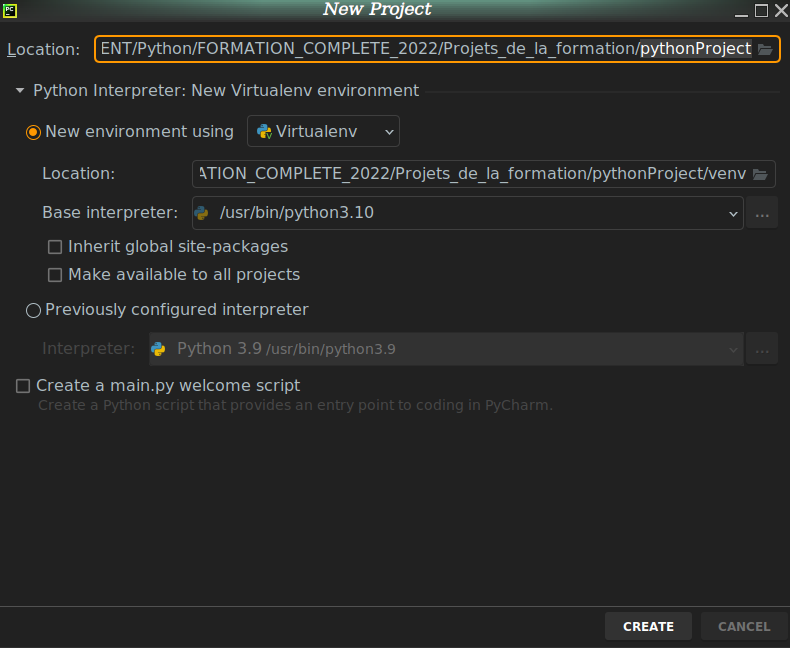
\includegraphics[scale=0.4]{IMG/Pycharm-12.png}
\caption{Interface \textit{New Project}}
\end{center}
\end{figure}
\medskip

\begin{enumerate}
	\item Choisir l'emplacement (\texttt{Location})
	\item Choisir l'interpréteur en cochant \texttt{New environnement using} et sélectionner \texttt{Virtualenv} qui utilise \texttt{venv}. \texttt{Location} permet de définir le répertoire où se situera la configuration virtuelle. Avec \texttt{Base interpreter} on choisit la version de \texttt{Python} à utiliser pour notre environnement virtuel.
	\item Choix optionnels:
	\begin{description}
		\item[Inherit global site-packages]: permet d'utiliser tous les paquets présents sur notre système.
		\item[More available to all projects]: permet de partager cet environnement virtuel avec d'autres projets.
	\end{description}
\end{enumerate}
\medskip

Vérifier que nous nous situons bien dans cet environnement virtuel en ouvrant le terminal dans \texttt{Pycharm}
\medskip

\section{Gérer plusieurs configurations (\texttt{pyenv})}
\subsection*{Installation de \texttt{pyenv} sous \texttt{Debian GNU/Linux}}
\begin{verbatim}
    # apt-get install-y make build-essential libssl-dev zliblg-dev libbz2-dev 
    	libreadline-dev libsqlite3-dev wget curl llvm libcurses5--dev libncurses-dev 
    	xz-utils tk-dev libffi-dev liblzma-dev python3-openssl
    $ curl -L https://raw.githubusercontent.com/yyuu/pyenv-installer/master/
    	binpyenv-installer | bash
\end{verbatim}
\medskip

Il est possible qu'à l'issue de l'installation on vous demande d'ajouter \texttt{pyenv} à votre \texttt{Path}, il suffit alors de suivre les instructions fournies. Un ajout des lignes proposées dans les fichiers \verb|~/.profile| et \verb|~/.bash.rc| ou \verb|~/.zshrc| devrait suffire. Pour vérifier l'installation et la version de \texttt{pyenv}:
\begin{verbatim}
    $ pyenv
\end{verbatim}
\medskip

\subsection*{Les principales commandes pour \texttt{pyenv}}
Voir quelle version de \texttt{Python} est utilisée:
\begin{verbatim}
    $ pyenv versions
\end{verbatim}
\medskip

Exemple de retour:
\begin{verbatim}
    * system (set by /home/krystof/.pyenv/version)
    3.8.0
    3.11.0b5
\end{verbatim}
\medskip

L'étoile (\texttt{*}) indique la version utilisée. Ici, il s'agit de la version utilisée par défaut par le système. Suivi de la commande \verb|$ python --version| nous connaîtrons la version de \texttt{Python} par défaut du système.
\medskip

Lister toutes les versions de \texttt{Python} qu'il est possible d'installer avec \texttt{pyenv}:
\begin{verbatim}
    $ pyenv install -l
\end{verbatim}
\medskip

Pour installer une version de \texttt{Python} (ici la \texttt{3.8.0}):
\begin{verbatim}
    $ pyenv install 3.8.0
\end{verbatim}
\medskip

Mais pour que cette version puisse être utilisée par défaut:
\begin{verbatim}
    $ pyenv 3.8.0
    $ pyenv rehash
\end{verbatim}
\medskip

Les deux commandes qui permettent d'effectuer des changements de version:
\begin{verbatim}
    $ pyenv rehash
    $ pyenv global [version]
\end{verbatim}
\medskip

%%%%%%%%%%%%
%%% Chapitre 3 %%%
%%%%%%%%%%%%
\chapter{Approfondir ses connaissances en algorithmie}
\section{\texttt{Codingame}}
Le site \texttt{Codingame} offre des exercices sous forme d'énigmes algorithmiques\footnote{\url{https://www.codingame.com/home}}. Il est possible de s'y inscrire via son profil \texttt{GitHub}.
\medskip

Pour afficher des sorties à l'aide de la fonction \texttt{print()}:
\begin{lstlisting}
import sys
print("Ce_que_l'on_souhaite_afficher", file=sys.stderr, flush=True)
\end{lstlisting}
\medskip

\chapter{Les messages d'erreur}


\section{\texttt{IndexError}}
\section{\texttt{KeyError}}
\section{\texttt{SyntaxError}}
\section{\texttt{TypeError}}
\section{\texttt{ValueError}}
\medskip

\part{\textcolor{cyan}{\texttt{Python} applicatif}}
\chapter{Manipuler des fichiers \texttt{.pdf}}
\section{La bibliothèque \texttt{PyPDF2}}
La bibliothèque \texttt{PyPDF2} est l'une des meilleures bibliothèques pour manipuler des fichiers \texttt{.pdf}. Elle permet à la fois de lire et d'écrire de tels fichiers, d'en extraire du texte et de combiner ensemble plusieurs fichiers. Il est aussi possible de réaliser une rotation des pages et des les superposer. Par contre, on ne peut rajouter du texte ou des marges.
\medskip

Installation:
\begin{verbatim}
    $ pip install PyPDF2==1.26.0
\end{verbatim}
\medskip

\section{Un premier script: combiner deux fichiers \texttt{.pdf} ensemble}
\begin{lstlisting}
"""Combiner deux fichiers .pdf.
Ce code suppose que vous disposiez de deux fichiers .pdf,
respectivement nommés 'fichier1.pdf' et 'fichier2.pdf'.
"""

from PyPDF2 import PdfFileWriter, PdfFileReader

# Création d'un fichier .pdf vide (en mémoire) :
contenu_sortie = PdfFileWriter()

# "rb" ouvrir en lecture un fichier binaire :
fichier_pdf_1 = open("fichier1.pdf", "rb")
fichier_pdf_2 = open("fihcier2.pdf", "rb")
# Lire les informations des fichiers
reader_pdf1 = PdfFileReader(fichier_pdf_1)
reader_pdf2 = PdfFileReader(fichier_pdf_2)
print(f"Nbre de pages du fichier recap : "
      f"{reader_pdf2.getNumPages()}")
# Combiner
# 1 - le fichier "fichier1.pdf" (0 pour première page) :
contenu_sortie.addPage(reader_pdf1.getPage(0))
# Et si nous voulions tourner le fichier de 90 degrés
# dans le sens des aiguilles d'une montre :
# contenu_sortie.addPage(reader_pdf1.getPage(0)).rotateClockwise(90)
# 2 - "fichier2.pdf" (toutes les pages via une boucle for) :
for i in range(reader_pdf2.getNumPages()):
    contenu_sortie.addPage(reader_pdf2.getPage(i))

# Ecrire notre fichier combiné :
fichier_combine = open("fichier_combine.pdf", "wb")
contenu_sortie.write(fichier_combine)

# Fermeture des fichiers
fichier_pdf_1.close()
fichier_pdf_2.close()
fichier_combine.close()
\end{lstlisting}
\medskip

\section{Extraire le texte d'un fichier \texttt{.pdf}}
L'extraction de base est assez simple:
\begin{lstlisting}
from PyPDF2 import PdfFileWriter, PdfFileReader

f = open("mon_fichier.pdf", "rb") 
reader = PdfFileReader(f)
page0 = reader.getPage(0)  # Extraction de la première page
texte = page0.extractText()  # Extraction du texte de la première page
f.close()

print(texte)  # Affichage du texte extrait
\end{lstlisting}
\medskip

Nous pouvons voir, qu'en sortie, le texte est extrait de manière brute, que nous avons perdu le style du fichier \texttt{.pdf} (on ne fait plus de distinction entre les titres et le corps du texte, par exemple). Ce qui est normal, puisque nous extrayons des chaînes de caractères.  Cependant nous avons un autre problème concernant l'affichage d'un certain nombre de caractères spéciaux, ainsi qu'avec les caractères accentués. De plus, si le fichier \texttt{.pdf} contient du texte dans les \textit{headers} celui-ci apparaît à la fin et non-plus en en-tête.
\medskip

Concernant les caractères spéciaux et caractères accentués, il va falloir étudier la sortie brute et à l'aide de la méthode replace(), venir remplacer un à un chaque caractère (user du copier/coller depuis la sortie). Notre code pourrait être alors le suivant:
\begin{lstlisting}
...
texte = page0.extractText()  # Extraction du texte de la première page
# On remplace chaque caractère un à un:
texte = texte.replace("Ò", '"').replace("'", "è")  # etc...
f.close()
...
\end{lstlisting}
\medskip

\chapter{Gérer des courriels}
\section{Envoyer un courriel}
\subsection*{Exemple avec un compte \texttt{Gmail}}
Il va tout d'abord nous falloir configurer le compte pour cela. Se rendre sur la \texttt{Gestion de compte}, puis à la section \texttt{Sécurité}. A \texttt{Connexion à Google}, activer la \texttt{Validation en deux étapes}. Ensuite: 
\begin{verbatim}
Mots de passe des applications > Sélectionner une application > Autre (personnalisé)
\end{verbatim}
\medskip

Donner un nom (Exemple: \og \textit{Avec Python}\fg{}) et cliquer sur \texttt{Générer}. Un mot de passe de seize caractères est alors généré, et c'est ce mot de passe que nous utiliserons dans nos codes.
\medskip

Chercher ensuite (via un moteur de recherche) la configuration \texttt{SMTP}\footnote{\textit{Simple Mail Transfert Protocol} (ou \textit{Protocole simple de transfert de courrier}: protocole de communication utilisé pour transférer le courrier électronique vers les serveurs de messagerie électronique.} de \texttt{Gmail}. Vous devriez trouver les éléments de configuration suivants:
\begin{description}
	\item[SMTP Server]: \texttt{smtp.gmail.com}
	\item[Server port]: \texttt{587}
\end{description}
\medskip

\subsection*{Envoyer un courriel simple}
Créer en premier lieu un projet contenant deux fichiers: \texttt{emails.py} (celui de notre programme principal) et config\_mail.py (fichier qui contiendra les paramètres et les informations confidentielles comme le mot de passe).
\medskip

Nous allons, pour mener à bien notre objectif, utiliser la bibliothèque \texttt{smtplib}.
\medskip

Voyons le code de nos deux fichiers:
\begin{lstlisting}[caption=\texttt{mails.py}]
"""Envoyer des mails avec gmail."""

import smtplib
import config_mail


def envoyer_mail(email_destinataire, message):
    serveur_mails = smtplib.SMTP(config_mail.config_server,
                                 config_mail.config_server_port)
    serveur_mails.starttls()  # Protocole de sécurité
    # Se connecter :
    serveur_mails.login(config_mail.config_email, 
                        config_mail.config_password)
    # Envoyer mail :
    serveur_mails.sendmail(config_mail.config_email, 
                           email_destinataire, message)
    serveur_mails.quit()  # Fermeture de la connexion


envoyer_mail("adresse_mail@destinataire.com", 
             "Ceci est un test avec Python")
\end{lstlisting}
\medskip

\begin{lstlisting}[caption=\texttt{config\_mail.py}]
config_email = "mail_émeteur@gmail.com"
config_password = "les_16_caractères_du_mot_de_passe_généré"
config_server = "smtp.gmail.com"
config_server_port = 587
\end{lstlisting}
\medskip

Pour envoyer un message contenu sur plusieurs lignes, il suffit d'attribuer le corps de notre message à une variable que l'on passera en paramètre lors de l'appel de la fonction \texttt{envoyer\_email()}:
\begin{lstlisting}[caption=Message sur plusieurs lignes]
corps_du_message = """Bonjour,
Ceci est un message rédigé à l'aide de Python.
A bientôt.
"""

envoyer_mail("adresse_mail@destinataire.com", corps_du_message)
\end{lstlisting}
\medskip

\subsection*{Un message \textit{mulitpart}}
Il s'agit d'un message auquel on ajoute des paramètres comme le sujet du courriel par exemple. Pour cela nous allons importer deux méthodes: \texttt{MIMEMultipart} et \texttt{MIMEText}.
\begin{lstlisting}[caption=Importer \texttt{MIMEMultipart} et \texttt{MIMEText}]
from email.mime.multipart import MIMEMultipart
from email.mime.text import MIMEText
\end{lstlisting}
\medskip

\texttt{MIME}, pour \og \textit{Multipurpose Internet Mail Extensions}\fg{} (ou \textit{Extensions multifontions du courrier Internet}), est un standard Internet qui étend le format de données des courriels pour supporter des textes en différents codages des caractères autres que l'\textit{ASCII}, des contenus non textuels, des contenus multiples et des informations d'en-tête. Les courriels, envoyés via le protocole \texttt{SMPTP} au format \texttt{MIME} sont appelés courriels \texttt{SMTP/MIME}.
\begin{lstlisting}[caption=Un courriel avec divers paramètres (\textit{multipart})]
"""Envoyer des mails avec gmail, et plusieurs paramètres."""

import smtplib
from email.mime.multipart import MIMEMultipart
from email.mime.text import MIMEText
import config_mail


def envoyer_mail(email_destinataire, sujet, message):
    multipart_message = MIMEMultipart()
    multipart_message["Subject"] = sujet
    multipart_message["From"] = config_mail.config_email
    multipart_message["To"] = email_destinataire
    # Attaché du texte plein
    # ("html" est possible - Intéressant pour les styles) :
    multipart_message.attach(MIMEText(message, "plain"))
    serveur_mails = smtplib.SMTP(config_mail.config_server,
                                 config_mail.config_server_port)
    serveur_mails.starttls()  # Protocole de sécurité
    # Se connecter :
    serveur_mails.login(config_mail.config_email, 
                        config_mail.config_password)
    # Envoyer mail :
    serveur_mails.sendmail(config_mail.config_email, 
                           email_destinataire,
                           multipart_message.as_string())
    serveur_mails.quit()  # Fermeture de la connexion


message_email = """Bonjour,

Voici un message généré avec Python.

Au revoir..."""
objet_email = "Email depuis Python"
mail_destinataire = input("Adresse mail du destinataire : ")
envoyer_mail(mail_destinataire, objet_email, message_email)
\end{lstlisting}
\medskip

\chapter{Le \textit{scraping}}
\section{Qu'est-ce que le \textit{scraping} ?}
Le \textit{scraping} permet d'extraire des données depuis des sites Web. Pour cela deux bibliothèques sont nécessaires: \texttt{requests} et \texttt{Beautiful Soup}.
\begin{description}
	\item[- \texttt{requests}]\footnote{\url{https://requests.readthedocs.io/en/latest/}} permet de réaliser ses requêtes \texttt{HTTP} et de récupérer le code source des pages \texttt{HTML}\footnote{L'\texttt{HTML} est un langage de balisage qui permet de décrire du contenu, notamment pour réaliser des pages Web. Cf \url{https://fr.wikipedia.org/wiki/Hypertext_Markup_Language}}.
	\item[- \texttt{Beautiful Soup}] va nous permettre de parcourir le code \texttt{HTML} afin d'y récupérer les données que l'on souhaite (comme le titre, du texte, la source d'une image, etc.).
\end{description}
\medskip

Tout ce qui est visible sur le Web peut potentiellement fournir des informations que l'on peut extraire.
\medskip

Depuis un navigateur on accède à un serveur via une requête \texttt{HTTP}. Ce serveur nous retourne des informations au format \texttt{HTML}, et le navigateur affiche alors une page Internet. Avec \texttt{Python} il est possible de développer une application qui va utiliser la bibliothèque \texttt{requests} afin de lancer des requêtes \texttt{HTTP} et ainsi de pouvoir récupérer les données \texttt{HTML} afin de les analyser et d'y extraire les informations voulues, cela à l'aide la bibliothèque \texttt{Beautiful Soup}. Il s'agit d'une méthode classique, mais il faut savoir qu'il existe aussi le \textit{framework} \texttt{Scrapy}\footnote{\url{https://scrapy.org/}} qui permet à la fois de lancer des requêtes \texttt{HTTP}, de récupérer les données du serveur et puis de les analyser. Avec \texttt{requests} et \texttt{Beautiful Soup} on demeure dans une démarche algorithmique.
\medskip

Il est à noter que certains sites se prémunissent contre le \textit{scraping}. Il est toutefois possible de contourner ces protections, et c'est ce que l'on nomme le \textit{Headless Browsing}\footnote{\url{https://fr.wikipedia.org/wiki/Navigateur_headless}}, mais cela s'apparente à du hacking.
\section{La bibliotèque \texttt{requests}: faire des appels réseaux}
Ce module fournit des fonctionnalités permettant de lancer des requêtes \texttt{HTTP}.
\medskip

Installer le module:
\begin{verbatim}
    $ pip install requests
\end{verbatim}
\medskip

\begin{lstlisting}[caption=Un premier exemple avec le module \texttt{requests}]
# FAIRE DES APPELS RESEAUX AVEC REQUESTS

# https://codeavecjonathan.com/res/programmation.txt
# https://codeavecjonathan.com/res/pizzas1.json
# https://codeavecjonathan.com/res/exemple.html

import requests
import json

# Récupérer du texte :
reponse = \ 
    requests.get(
        "https://codeavecjonathan.com/res/programmation.txt")
reponse.encoding = "utf-8"
print(reponse.text)

# Récupérer des données au format .json :
reponse = \
    requests.get(
        "https://codeavecjonathan.com/res/pizzas1.json")
# Pour une gestion de l'erreur si la page web 
# ne devait pas exister :
if reponse.status_code == 200:
    reponse.encoding = "utf-8"
    print(reponse.text)
    pizzas = json.loads(reponse.text)
    print(f"Nombre de pizzas : {len(pizzas)}")
else:
    print(f"ERREUR Code : {reponse.status_code}")

# Récupérer le code source d'un site :
reponse = \
    requests.get(
        "https://codeavecjonathan.com/res/exemple.html")
reponse.encoding = "utf-8"
print(reponse.text)
\end{lstlisting}
\medskip

La fonction \texttt{.get()} permet de récupérer du code \texttt{HTML}.
\medskip

\begin{lstlisting}[caption=Télécharger une image avec le module \texttt{requests}]
# TELECHARGER UNE IMAGE AVEC REQUESTS

# https://codeavecjonathan.com/res/papillon.jpg

import requests

reponse = \
    requests.get(
        "https://codeavecjonathan.com/res/papillon.jpg")
if reponse.status_code == 200:
    # Ouverture en écriture binaire :
    f = open("papillon.jpg", "wb")  
    f.write(reponse.content)
    f.close()
    print("Ecriture terminée")
else:
    print(f"ERREUR : {reponse.status_code}")
\end{lstlisting}
\medskip

\section{La bibliothèque \texttt{Beautiful Soup}: extraire des données depuis un simple fichier \texttt{.html}}
\begin{verbatim}
    $ pip install beautifulsoup4
\end{verbatim}
\medskip

Commençons par créer un projet, un répertoire contenant à la fois le fichier .py qui contiendra notre code et un fichier .html qui contiendra les éléments à extraire.
\medskip

Le fichier \texttt{livre.html}:
\begin{verbatim}
<h1>Pour Qui sonne le Glas</h1>

<table border="1">
    <tr>
        <th>Auteur</th>
        <th>Date de publication</th>
    </tr>
    <tr>
        <td>Ernest Hemingway</td>
        <td>1940</td>
    </tr>
</table>

<p>'Pour qui sonne le glas' est un roman d'Ernest Hemingway fortement 
inspiré de son vécu de journaliste pendant la guerre civile espagnole. </p>

<img src="https://upload.wikimedia.org/wikipedia/commons/thumb/2/28/ErnestHe
mingway.jpg/220px-ErnestHemingway.jpg">
\end{verbatim}
\medskip

Il est parfois cependant difficile de lire le code source d'un fichier \texttt{.html}. Nous pouvons alors faire appel à un formateur de code \texttt{html}\footnote{Voir par exemple: \url{https://www.site24x7.com/fr/tools/html-formateur.html}}.
\medskip

De même le code récupéré à l'aide du module \texttt{requests} est illisible. Il va donc falloir \textit{parser}\footnote{Parcourir le contenu d'un fichier en l'analysant pour vérifier sa syntaxe ou en extraire des éléments.} ce qui a été récupéré à l'aide du module \texttt{BeautifulSoup}. On \textit{parse} du \texttt{HTML} avec les attributs \texttt{HTML} \texttt{class} et \texttt{id}.
\medskip

Le fichier \texttt{extraction.py}:
\begin{lstlisting}[caption=Exemple simple d'extraction avec \texttt{Beautiful Soup}]
# Import de la classe 'BeautifulSoup':
from bs4 import BeautifulSoup  

# Lecture des données HTML :
f = open("livre.html", "r")  # Ouverture fichier .html en local
html_content = f.read()  # Lecture du fichier .html
f.close()
soup = BeautifulSoup(html_content, "html.parser")

# Extractions:
titre_h1 = soup.find("h1")  # Chercher l'occurence "h1"
description_p = soup.find("p")  # Un texte
image_src = soup.find("img")  # Source de l'image
texte_titre = titre_h1.text  # Récupérer le texte

# Affichage des extractions:
print(f"Titre de la page HTML: {texte_titre}")
# Ou bien -> print(f"Titre de la page HTML: {titre_h1.text}")
print(f"Texte descritptif: {description_p.text}")
print(f"Le fichier source de l'image est: {image_src['src']}")
\end{lstlisting}
\medskip

La ligne:
\begin{lstlisting}
soup = BeautifulSoup(html_content, "html.parser")
\end{lstlisting}
permet de créer un objet \og \textit{soup}\fg{} à partir du \texttt{HTML} récupéré. La variable \texttt{soup} possède alors toutes les fonctions qui facilitent l'obtention de données à partir de l'\texttt{HTML}.
\medskip 

\section{Transformer les données à l'aide du module \texttt{csv}}
Il existe différentes façons de transformer des données. Cela va dépendre du type de données et du format souhaité en sortie.
\medskip

Voir la lecture et l'écriture de fichiers \texttt{.csv}\footnote{\url{https://docs.python.org/fr/3/library/csv.html}}
\medskip

\subsection*{La méthode \texttt{.reader}}
Va analyser tout le texte dans un fichier \texttt{.csv}, le \textit{parser} ligne par ligne et convertir chaque ligne dans une liste de chaîne de caractères. Pour le délimiteur de colonnes, on peut choisir n'importe quel signe, mais la virgule est communément employée.
\medskip

Prenons comme exemple le fichier \texttt{.csv} suivant, contenant les noms de communes du canton de Lescar\footnote{\url{https://fr.wikipedia.org/wiki/Canton_de_Lescar}}, avec les distances qui séparent chaque commune de celle de Lescar:
\begin{verbatim}
    commune,distance_km_depuis_Lescar
    Arbus,8.8 
    Artiguelouve,4.6
    Aussevielle,5.4
    Beyrie-en-Béarn,7.3
    Bougarber,9
    Caubios-Loos,11
    Denguin,7.5
    Lescar,0
    Lons,4.4
    Momas,15
    Poey-de-Lescar,4.8
    Sauvagnon,10
    Siros,4.8
    Uzein,9.7
\end{verbatim}
\medskip

\begin{lstlisting}[caption=La méthode \texttt{.reader()}]
import csv

with open('communes_canton_Lescar.csv') as fichier_csv:
    reader = csv.reader(fichier_csv, delimiter=',')
    for ligne in reader:
        print(ligne)
\end{lstlisting}
\medskip

En sortie, cela donnera:
\begin{verbatim}
    ['commune', 'distance_km_depuis_Lescar']
    ['Arbus', '8.8']
    ['Artiguelouve', '4.6']
    ['Aussevielle', '5.4']
    ['Beyrie-en-Béarn', '7.3']
    ['Bougarber', '9']
    ['Caubios-Loos', '11']
    ['Denguin', '7.5']
    ['Lescar', '0']
    ['Lons', '4.4']
    ['Momas', '15']
    ['Poey-de-Lescar', '4.8']
    ['Sauvagnon', '10']
    ['Siros', '4.8']
    ['Uzein', '9.7']
\end{verbatim}
\medskip

\subsection*{La méthode \texttt{.DictReader()}}
Avec la méthode \texttt{.reader} la ligne d'en-tête est considérée à l'instar des autres. Avec la méthode \texttt{.DictReader()} la ligne d'en-tête va être utilisée pour générer les clés du dictionnaire qui contiendra les valeurs de chaque ligne.
\medskip

\begin{lstlisting}[caption=La méthode \texttt{.DictReader()}]
import csv

with open('communes_canton_Lescar.csv') as fichier_csv:
    reader = csv.DictReader(fichier_csv, delimiter=',')
    for ligne in reader:
        print(ligne) # Sous forme d'un dictionnaire
        # Générer un texte:
        print(f"La commune de {ligne['commune']} est distante "
              f"de {ligne['distance_km_depuis_Lescar']} km "
              f"depuis Lescar")
\end{lstlisting}
\medskip

En sortie:
\begin{verbatim}
    {'commune': 'Arbus', 'distance_km_depuis_Lescar': '8.8'}
    La commune de Arbus est distante de 8.8 km depuis Lescar
    {'commune': 'Artiguelouve', 'distance_km_depuis_Lescar': '4.6'}
    La commune de Artiguelouve est distante de 4.6 km depuis Lescar
    {'commune': 'Aussevielle', 'distance_km_depuis_Lescar': '5.4'}
    La commune de Aussevielle est distante de 5.4 km depuis Lescar
    {'commune': 'Beyrie-en-Béarn', 'distance_km_depuis_Lescar': '7.3'}
    La commune de Beyrie-en-Béarn est distante de 7.3 km depuis Lescar
    {'commune': 'Bougarber', 'distance_km_depuis_Lescar': '9'}
    La commune de Bougarber est distante de 9 km depuis Lescar
    {'commune': 'Caubios-Loos', 'distance_km_depuis_Lescar': '11'}
    La commune de Caubios-Loos est distante de 11 km depuis Lescar
    {'commune': 'Denguin', 'distance_km_depuis_Lescar': '7.5'}
    La commune de Denguin est distante de 7.5 km depuis Lescar
    {'commune': 'Lescar', 'distance_km_depuis_Lescar': '0'}
    La commune de Lescar est distante de 0 km depuis Lescar
    {'commune': 'Lons', 'distance_km_depuis_Lescar': '4.4'}
    La commune de Lons est distante de 4.4 km depuis Lescar
    {'commune': 'Momas', 'distance_km_depuis_Lescar': '15'}
    La commune de Momas est distante de 15 km depuis Lescar
    {'commune': 'Poey-de-Lescar', 'distance_km_depuis_Lescar': '4.8'}
    La commune de Poey-de-Lescar est distante de 4.8 km depuis Lescar
    {'commune': 'Sauvagnon', 'distance_km_depuis_Lescar': '10'}
    La commune de Sauvagnon est distante de 10 km depuis Lescar
    {'commune': 'Siros', 'distance_km_depuis_Lescar': '4.8'}
    La commune de Siros est distante de 4.8 km depuis Lescar
    {'commune': 'Uzein', 'distance_km_depuis_Lescar': '9.7'}
    La commune de Uzein est distante de 9.7 km depuis Lescar
\end{verbatim}
\medskip

\section{Les problèmes éthiques de l'extraction \textit{Web}}
Pour visualiser ce qui est extractables des sites \textit{Web} il faut se référer à leur fichier \texttt{robots.txt}\footnote{\url{https://robots-txt.com/}} s'il existe. Il faut alors ajouter l'extension \texttt{/robots.txt} après l'\textit{URL} d'un site. Exemple:
\begin{verbatim}
    https://www.docstring.fr/robots.txt
\end{verbatim}
\medskip

\section{Les défis de l'extraction \textit{Web}}
\begin{itemize}
	\item[-] La variété des sites \textit{Web} avec des instructions \texttt{HTML} différentes.
	\item[-] La durabilité des scripts, en lien avec les changements des structures \texttt{HTML} des sites.
\end{itemize}
\medskip

\chapter{Télécharger des fichiers audio et vidéo depuis \textit{Youtube}}
Nous allons coder un petit projet permettant de télécharger une vidéo depuis \textit{Youtube}, en sélectionnant la meilleure qualité qui  soit.
\medskip

\section{Création du projet et installation des modules et paquets nécessaires}
Tout d'abord il nous sera nécessaire de créer un projet à l'aide d'un environnement virtuel. Ensuite nous installerons dans cet environnement les modules suivants:
\begin{description}
	\item[Pytube]\footnote{Voir la page \textit{GitHub} du projet: \url{https://github.com/pytube/pytube}. Pour la documentation on se référera à la page suivante: \url{https://pytube.io/en/latest/api.html}}: c'est le module incontournable pour télécharger des fichiers audio et vidéo depuis \textit{Youtube}. Ce module se télécharge à partir des sources\footnote{Voir: \url{https://github.com/pytube/pytube\#installation}}.
	\item[ffmpeg.python]\footnote{Voir la page \textit{Github} du projet: \url{https://github.com/kkroening/ffmpeg-python}}: ce module permet de regrouper des fichiers audio et vidéo séparés. Son utilisation nécessite l'installation sur le système du package \textit{ffmpeg}.
\end{description}
\medskip

Installons donc tout cela:
\begin{verbatim}
    # pip3 install git+https://github.com/pytube/pytube
    # aptitude install ffmpeg
    # pip3 install ffmpeg-python
\end{verbatim}
\medskip

\section{Le code du projet}
Le projet se compose de deux fichiers: \textit{main.py} et \textit{yt\_downloader.py}.

\begin{lstlisting}[caption=Le fichier \textit{main.py}]
import yt_downloader

urls = ("https://www.youtube.com/watch?v=BNdcOOsrHOs&list=
            PL44A0E4C7FFA5B749&index=1",
        "https://www.youtube.com/watch?v=NxjuOJkXAq0&list=
            PL44A0E4C7FFA5B749&index=2",
        "https://www.youtube.com/watch?v=qdYwrFRxKH0&list=
            PL44A0E4C7FFA5B749&index=3",
        "https://www.youtube.com/watch?v=_lZPlQiV4ps&list=
            PL44A0E4C7FFA5B749&index=4",
        "https://www.youtube.com/watch?v=Sg-FFmwT2jE&list=
            PL44A0E4C7FFA5B749&index=5",
        "https://www.youtube.com/watch?v=4jCxP0d5BtI&list=
            PL44A0E4C7FFA5B749&index=6")

for url in urls:
    yt_downloader.download_video(url)
\end{lstlisting}
\medskip

Vous pouvez bien entendu changer les \textit{url} des pages \textit{Youtube}. Il s'agit ici de six titres du groupe \textit{The Cure} en version acoustique.
\medskip

\begin{lstlisting}[caption=Le fichier \textit{yt\_downloader.py}]
import os
from pytube import YouTube
import ffmpeg


def progression_telechargement(the_stream, chunk, 
                               bytes_remainnig):
    """Affichage en pourcentage de la progression du 
    téléchargement.
    """
    # Nbre octets au total - nbre octets restant :
    bytes_telecharges = the_stream.filesize - bytes_remainnig
    pourcentage = bytes_telecharges * 100 / the_stream.filesize
    # int() pour avoir des nbres entiers :
    print(f"Progession du téléchargement : "
          f"{int(pourcentage)}%")


def download_video(url):
    ma_video_yt = YouTube(url)  # Création objet 'YouTube'.
    # Affichage informations :
    print(f"TITRE : {ma_video_yt.title}")
    # Utilisation filtre pour avoir les meilleures résolutions :
    streams_video = ma_video_yt.streams.filter(
        progressive=False, file_extension='mp4',
        type="video").order_by("resolution").desc()
    streams_audio = ma_video_yt.streams.filter(
        progressive=False, file_extension='mp4',
        type="audio").order_by("abr").desc()
    meilleur_stream_video = streams_video[0]
    meilleur_stream_audio = streams_audio[0]
    # Pour afficher la progression du téléchargement :
    ma_video_yt.register_on_progress_callback(
        progression_telechargement)
    # Téléchargement :
    print(f"Téléchargement de la vidéo "
          f"'{ma_video_yt.title}'...")
    meilleur_stream_video.download("Video")
    meilleur_stream_audio.download("Audio")
    # Combiner le fichier vidéo et le fichier audio :
    audio_filename = os.path.join(
        "Audio", meilleur_stream_video.default_filename)
    video_filename = os.path.join(
        "Video", meilleur_stream_video.default_filename)
    output_filename = meilleur_stream_video.default_filename
    ffmpeg.output(ffmpeg.input(audio_filename), 
                  ffmpeg.input(video_filename),
                  output_filename, vcodec="copy", 
                  acodec="copy", 
                  loglevel="quiet").run(overwrite_output=True)
    print(f"Fin du téléchargement de la vidéo "
          f"'{ma_video_yt.title}'")
    # Suppression des fichiers temporaires :
    os.remove(audio_filename)
    os.remove(video_filename)
    os.rmdir("Audio")
    os.rmdir("Video")
\end{lstlisting}
\medskip

\section{Les extractions}
Pour visualiser ce que nous pouvons extraire de l'objet \og \textit{Youtube}\fg{} (ici, notre objet se nomme \texttt{ma\_video\_yt}), à l'aide du debogger nous pouvons placer un point d'arrêt juste après la création de l'objet (situer le point d'arrêt ligne 22). Nous pouvons alors voir que nous disposons de divers éléments d'informations que nous pouvons obtenir de la façon suivante:
\begin{verbatim}
    ma_video_yt.méthode
\end{verbatim} 
\medskip

Voyons quelques uns de ces champs (ou méthodes):
\begin{description}
	\item[\texttt{itag}]: identifiant du \textit{stream}.
	\item[\texttt{mine\_type}]: type de fichier.
	\item[\texttt{res}]: résolution (pour les fichiers vidéo).
	\item[\texttt{abr}]: qualité sonore (pour les fichiers audio).
	\item[\texttt{fps}]: nombre d'images par seconde (plus ce nombre est important, plus la vidéo est fluide).
	\item[\texttt{vcodec} et \texttt{acodec}]: différents codecs.
	\item[\texttt{progressive}]: \texttt{True} pour les fichiers contenant à la fois le flux audio et le flux vidéo. \texttt{False} ne prendra en compte que les fichiers audio et vidéo séparés (il sera nécessaire de combiner ces fichiers pour avoir les deux flux dans un même fichier, c'est ce que permet le module \texttt{ffmpeg-python}).
\end{description}
\medskip

\section{Enregistrer la progression d'un téléchargement}
A noter que si le fichier souhaité est déjà téléchargé, relancer le programme ne lancera pas le téléchargement.
\medskip

L'enregistrement de la progression se situe au niveau de la fonction \\ \texttt{progression\_telechargement} du fichier \texttt{yt\_downloader.py}. Voir aussi la ligne 33 pour l'appel de cette fonction.
\medskip

Voir la documentation idoine\footnote{\url{https://pytube.io/en/latest/api.html\#pytube.YouTube.register\_on\_progress\_callback} et \url{https://pytube.io/en/latest/\_modules/pytube/\_\_main\_\_.html\#YouTube.register\_on\_progressive\_callback}}.
\medskip

La section \textit{API} de la documentation liste toutes les fonctions du module. La méthode \texttt{register\_on\_progress\_callback} permet d'enregistrer une fonction \textit{callback} (fonction appelée par la fonction) relative à la progression du téléchargement après l'initialisation. Ce qui va nous intéresser c'est la valeur de \texttt{bytes\_remaining} qui correspond au nombre d'octets à télécharger, et à l'aide de cette valeur nous pourrons calculer la durée restante de téléchargement.
\medskip

\section{Faire évoluer ce projet}
A partir de ce projet de base nous pouvons imaginer divers évolutions: permettre l'insertion d'\textit{url} par l'utilisateur, choix du type de fichier à télécharger, choix des répertoires d'enregistrement, implémentation d'une interface graphique, renommer les fichiers téléchargés, et j'en passe.
\medskip

\part{\textcolor{cyan}{\textit{Python} en mode graphique}}
\chapter{Jouons avec la tortue}
\section{Introduction}
Nous allons donc déplacer la tortue (\textit{turtle}) à l'aide des quatre commandes de base qui sont: \texttt{forward} (avancer), \texttt{backward} (reculer), \texttt{right} (tourner à droite) et \textit{left} (tourner à gauche). On va pouvoir écrire un programme qui utilise de façon séquentielle les commandes citées.
\medskip

La première chose à faire est d'importer le module \texttt{turtle} et d'initialiser notre tortue.
\begin{lstlisting}[caption=Les trois lignes d'initialisation de notre fenêtre graphique]
  import turtle
  # Initialisation de notre 'turtle' avec la variable 't':
  t = turtle.Turtle()
  # De façon à garder la fenêtre active:
  turtle.done()
\end{lstlisting}
\medskip

Rien qu'avec ce code, une fenêtre graphique s'ouvre avec notre tortue au centre.
\medskip

\begin{figure}[h]
\begin{center}
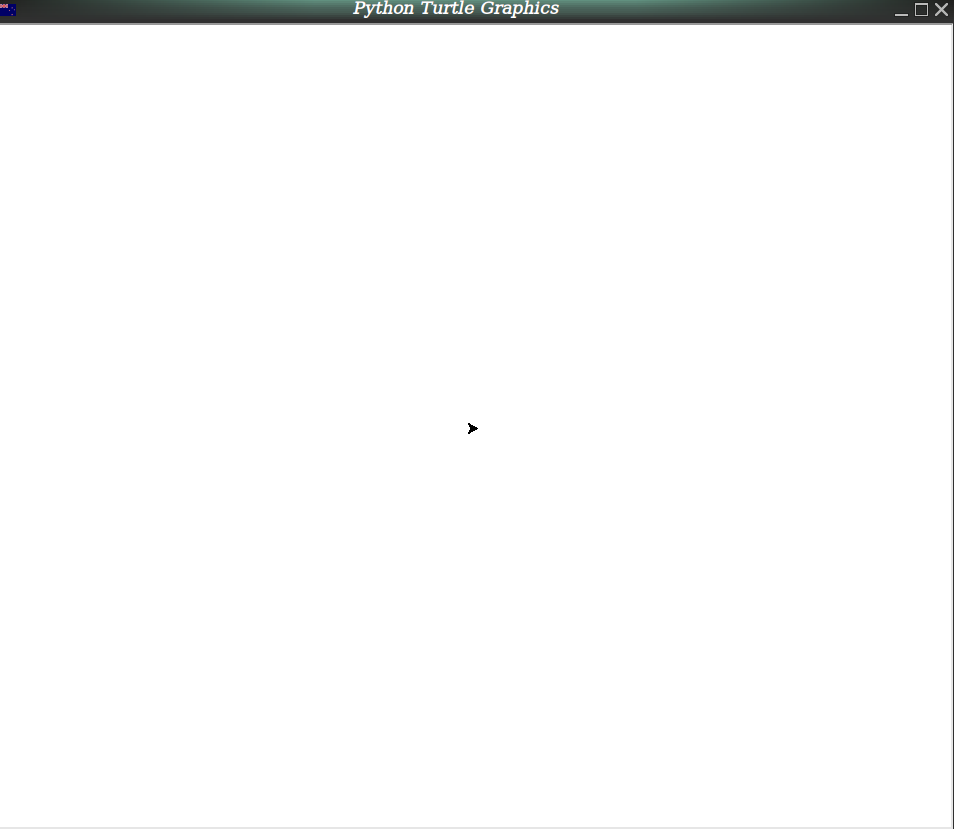
\includegraphics[scale=0.15]{IMG/turtle-01.png}
\caption{La fenêtre graphique et la tortue}
\end{center}
\end{figure}
\medskip

Faisons maintenant avancer et tourner notre tortue, puis avancer à nouveau, etc.
\begin{lstlisting}[caption=La tortue se déplace]
  import turtle
  t = turtle.Turtle()
  # Faisons bouger notre tortue
  t.forward(100)  # Avancer de 100 pixels
  t.left(90)  # Tourner à gauche de 90 degrés
  t.forward(50)
  t.backward(100)  # Reculer de 100 pixels
  t.right(45)  # Tourner à droite de 45 degrés
  t.forward(200)
  turtle.done()
\end{lstlisting}
\medskip

\begin{figure}[h]
\begin{center}
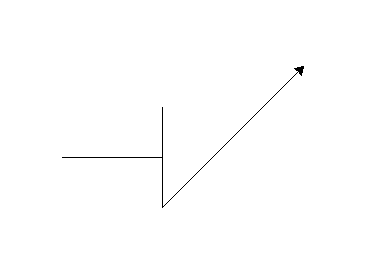
\includegraphics[scale=0.4]{IMG/turtle-02.png}
\caption{Premiers déplacements de la tortue}
\end{center}
\end{figure}
\medskip

\section{Un escalier}
Dessin d'un escalier avec des marches de 30 pixels de largeur et de hauteur, avec 5 marches au total.
\begin{lstlisting}
"""Dessin d'un escalier avec le module 'turtle' :
- 5 marches de 30 pixels."""

import turtle

t = turtle.Turtle()
nbre_pixels = 30
angle = 90
nbre_marches = 5


def escalier(nb_px, ang, nb_m):
    """Dession de l'escalier"""
    for i in range(0, nb_m):
        t.left(ang)
        t.forward(nb_px)
        t.right(ang)
        t.forward(nb_px)


# Pour la première marche
t.forward(nbre_pixels)
# Pour toutes les autres marches
escalier(nbre_pixels, angle, nbre_marches)

turtle.done()
\end{lstlisting}
\medskip

\section{Dessin de plusieurs carrés de tailles différentes}
\begin{lstlisting}
"""Dessin d'un carré de 100 pixels de côté"""

import turtle

nbre_pixels = 50
nbre_carres = 8
t = turtle.Turtle()


def carre(nb_px):
    for i in range(0, 4):
        t.forward(nb_px)
        t.left(90)


def carres(taille1, nb_carres):
    for i in range(0, nb_carres):
        taille1 += 20
        carre(taille1)


carres(nbre_pixels, nbre_carres)

turtle.done()
\end{lstlisting}
\medskip

\part{Une bibliothèque riche et dense}
\chapter{Générer des données aléatoires avec le module \texttt{random}}

\section{Les \textit{PRNGs} en \textit{Python}}
Il s'agit en fait de données \textit{pseudo-aléatoires}. Cela signifie qu'elles sont générées par un générateur de nombres pseudo-aléatoires (\textit{PRNG}), c'est-à-dire tout algorithme permettant de générer de telles données, apparemment aléatoires, est néanmoins reproductible. Les \og vrais\fg{} nombres aléatoires sont quant à générés par un véritable générateur de nombres aléatoires (\textit{TRNG}). Les \textit{PRNG}, sont généralement réalisés avec un logiciel plutôt qu'avec du matériel, et ils fonctionnent de manière légèrement différente des \textit{TRNG}\footnote{Pour plus d'informations à ce sujet: \url{https://learn.microsoft.com/fr-fr/windows/win32/api/wincrypt/nf-wincrypt-cryptgenrandom?redirectedfrom=MSDN}}. C'est pour cette raison que dans la documentation officielle du module\footnote{Module \texttt{random}: https://docs.python.org/fr/3/library/random.html} on y trouve l'avertissement suivant: \og \textit{Les générateurs pseudo-aléatoires de ce module ne doivent pas être utilisés à des fins de sécurité}\fg{}\footnote{Pour générer des nombres aléatoires de façon sécurisée, on se tournera vers le module \texttt{secrets}: \url{https://docs.python.org/fr/3.11/library/secrets.html}}.  
\medskip

L'outil le plus connu pour générer des données aléatoires en \textit{Python} est probablement le module \texttt{random}, qui utilise l'algorithme \textit{PRNG} \texttt{Mersenne Twister}\footnote{\url{https://github.com/python/cpython/blob/main/Modules/_randommodule.c}} comme générateur de base.

\section{\texttt{random.random()} et \texttt{random.seed()}}
Tout d'abord, construisons des données aléatoires sans recourir à la technique de l'ensemencement (\texttt{random.seed()}). La fonction \texttt{random.random()} renvoie un nombre flottant aléatoire dans l'intervalle \texttt{[0.0, 1.0]}. Le résultat sera toujours inférieur à l'extrémité droite \texttt{(1,0)}. C'est ce qu'on appelle un intervalle semi-ouvert : 
\begin{verbatim}
    >>> import random
    >>> random.random()
    0.6179433636795252
    >>> random.random()
    0.2533837287218852
\end{verbatim}
\medskip

On voir ici que les résultats obtenus sont différents. Avec \texttt{random.seed()}, il est possible de rendre les résultats reproductibles:
\begin{verbatim}
    >>> random.seed(444)
    >>> random.random()
    0.3088946587429545
    >>> random.random()
    0.01323751590501987
    >>> random.seed(444)
    >>> random.random()
    0.3088946587429545
    >>> random.random()
    0.01323751590501987
\end{verbatim}
\medskip

Avec \texttt{random.seed()} la séquence de nombres aléatoires devient déterministe, ou complètement déterminée par la valeur de départ (ici \texttt{444}).

\section{\texttt{random.randint()} et \texttt{random.randrange()}}
Il est possible de générer un nombre entier aléatoire, compris entre deux points d'extrémité, à l'aide de la fonction \texttt{random.randint()}. Cette fonction couvre l'ensemble de l'intervalle \texttt{[x, y]}:
\begin{verbatim}
    >>> random.randint(0, 10)
    10
    >>> random.randint(500, 50000)
    49829
\end{verbatim}
\medskip

Avec \texttt{random.randrange()}, nous excluons le côté droit de l'intervalle, ce qui signifie que le nombre généré se situe toujours à l'intérieur de \texttt{[x, y]} et sera toujours plus petit que la valeur \texttt{y}:
\begin{verbatim}
    >>> random.randrange(0, 3)
    1
    >>> random.randrange(0, 3)
    1
    >>> random.randrange(0, 3)
    0
    >>> random.randrange(0, 3)
    2
    >>> random.randrange(0, 3)
    1
\end{verbatim}
\medskip

\section{\texttt{random.uniform()}}
Si nous avons besoin de générer des valeurs flottantes aléatoires comprises dans un intervalle \texttt{[x, y]} spécifique, nous utiliserons \texttt{random.uniform()}:
\begin{verbatim}
    >>> random.uniform(10, 15)
    10.598997942362535
    >>> random.uniform(10, 15)
    13.969776294398033
\end{verbatim}

\section{\texttt{random.choice()}, \texttt{random.choices()}, \texttt{random.sample()} et \\ \texttt{random.shuffle()}: des outils pour les séquences}
Pour choisir un élément aléatoire dans une séquence non vide (comme une liste ou un tuple), nous pouvons utiliser \texttt{random.choice()}. Il existe également \texttt{random.choices()} pour choisir plusieurs éléments d'une séquence (à noter que les doublons sont possibles) :
\begin{verbatim}
    >>> items = ['un', 'deux', 'trois', 'quatre', 'cinq']
    >>> random.choice(items)
    'un'
    >>> random.choice(items)
    'quatre'
    >>> random.choices(items, k=2)
    ['un', 'cinq']
    >>> random.choices(items, k=3)
    ['un', 'un', 'cinq']
    >>> random.choices(items, 3)  # Avec absence du mot-clé de l'argument
    Traceback (most recent call last):
      File "<stdin>", line 1, in <module>
      File "/usr/lib/python3.11/random.py", line 500, in choices
        raise TypeError(
    TypeError: The number of choices must be a keyword argument: k=3
\end{verbatim}
\medskip

Pour éviter les doublons il sera préférable de faire appel à \texttt{random.sample()}:
\begin{verbatim}
    >>> random.sample(items, 4)
    ['trois', 'cinq', 'un', 'quatre']
    >>> random.sample(items, 4)
    ['un', 'trois', 'deux', 'quatre']
    >>> random.sample(items, 4)
    ['trois', 'deux', 'un', 'quatre']
    >>> random.sample(items, 4)
    ['cinq', 'un', 'quatre', 'deux']
\end{verbatim}
\medskip

Nous pouvons modifier l'ordre d'une séquence sur place à l'aide de \texttt{random.shuffle()}. Cette méthode modifie l'objet séquence et modifie l'ordre des éléments de manière aléatoire :
\begin{verbatim}
    >>> random.shuffle(items)
    >>> items
    ['cinq', 'un', 'quatre', 'deux', 'trois']
\end{verbatim}
\medskip

\end{document}


